\chapter{Εντοπισμός Σημείων Αλλαγής με Μη-Γραμμικά Μοντέλα}
\label{ch:step6}
\thispagestyle{fancy}

\section{Ανακτασκευή του χώρου καταστάσεων}

Για την ανακατασκευή του χώρου καταστάσεων (όπως περιγράφεται στις σημειώσεις του κ. Κουγιουμτζή - σελίδες 90-92) θα χρησιμοποίησουμε την \textit{μέθοδο των υστερήσεων}. Επομένως χρειαζόμαστε σημεία  $\mathbf{x_i} \in \mathbb{R}^m$ τα οποία προκύπτουν από τις (μονοδιάστατες) παρατηρήσεις της εκάστοτε χρονοσειράς με βάση τη ακόλουθη σχέση (σχέση 97 σελ. 91):
\begin{align}
    \mathbf{x}_i = \left[x_i, x_{i-\tau}, ..., , x_{i-(m-1)\tau}\right]
\end{align}
Το πρώτο πράγμα που απαιτείται να γίνει πριν την προσαρμογή οποιουδήποτε μη-γραμμικού μοντέλου σε χρονοσειρά που βασίζεται στην ύπαρξη συνάρτησης παρατήρησης της τροχίας στο χώρο καταστάσεων, είναι η εκτίμηση των παραμέτρων ανακατασκευής, ως εξής:
\begin{itemize}
    \item \textit{Διάστασης Εμβύθισης Ελκυστή, \textbf{\tl{m}}}: θα οριστεί με βάση τη μέθοδο των ψευδών κοντινότερων γειτόνων (\tl{false nearest neighbors - FNN}), όπως προτείνεται στη σελ. 92 των σημειώσεων
    \item \textit{Υστέρηση, $\mathbf{\tau}$}: θα οριστεί από τη συνάρτηση αμοιβαίας πληροφορίας (\tl{mutual information - $I(\tau)=I(x_i,x_{i-\tau}$}), όπως προτείνεται στις σελ. 91-92 των σημειώσεων
\end{itemize}

\par Στο σημείο αυτό, κρίνεται σκόπιμο να τονιστεί ότι η όλη ανάλυση γίνεται για τις στάσιμες χρονοσειρές που προέκυψαν από την ανάλυση των βημάτων \ref{ch:step2} και \ref{ch:step3}. Δηλαδή, αντί για την αρχική χρονοσειρά των προβολών του βίντεο \tl{A}, $\{Y_a(t)\}$, θα ασχοληθούμε με τη στάσιμη εκδοχή της, $\{X_a(t)\}$, σχέση (\ref{eq:xa_t}). Εντελώς παρόμοια, αντί για την αρχική χρονοσειρά των προβολών του βίντεο \tl{B}, $\{Y_b(t)\}$, θα ασχοληθούμε με τη στάσιμη εκδοχή της, $\{X_{b_deseasoned}(t)\}$, σχέση (\ref{eq:xb_ds_t}).

\subsection{Παράμετροι ανακατασκευής για τη Χρονοσειρά \tl{A}}

\subsubsection{Υστέρηση, τ}

Για την εύρεση της υστέρησης, $\tau$, θα χρησιμοποιήσουμε την συνάρτηση αμοιβαίας πληροφορίας και θα αναζητήσουμε το πρώτο τοπικό της ελάχιστο (ως προς την υστέρηση). Ακολούθως, δίνεται το διάγραμμα της αμοιβαίας πληροφορίας, $I_a(\tau)$, και παραθέτεται η επιλεγμένη τιμή για την υστέρηση.

\begin{figure}[H]
    \begin{center}
        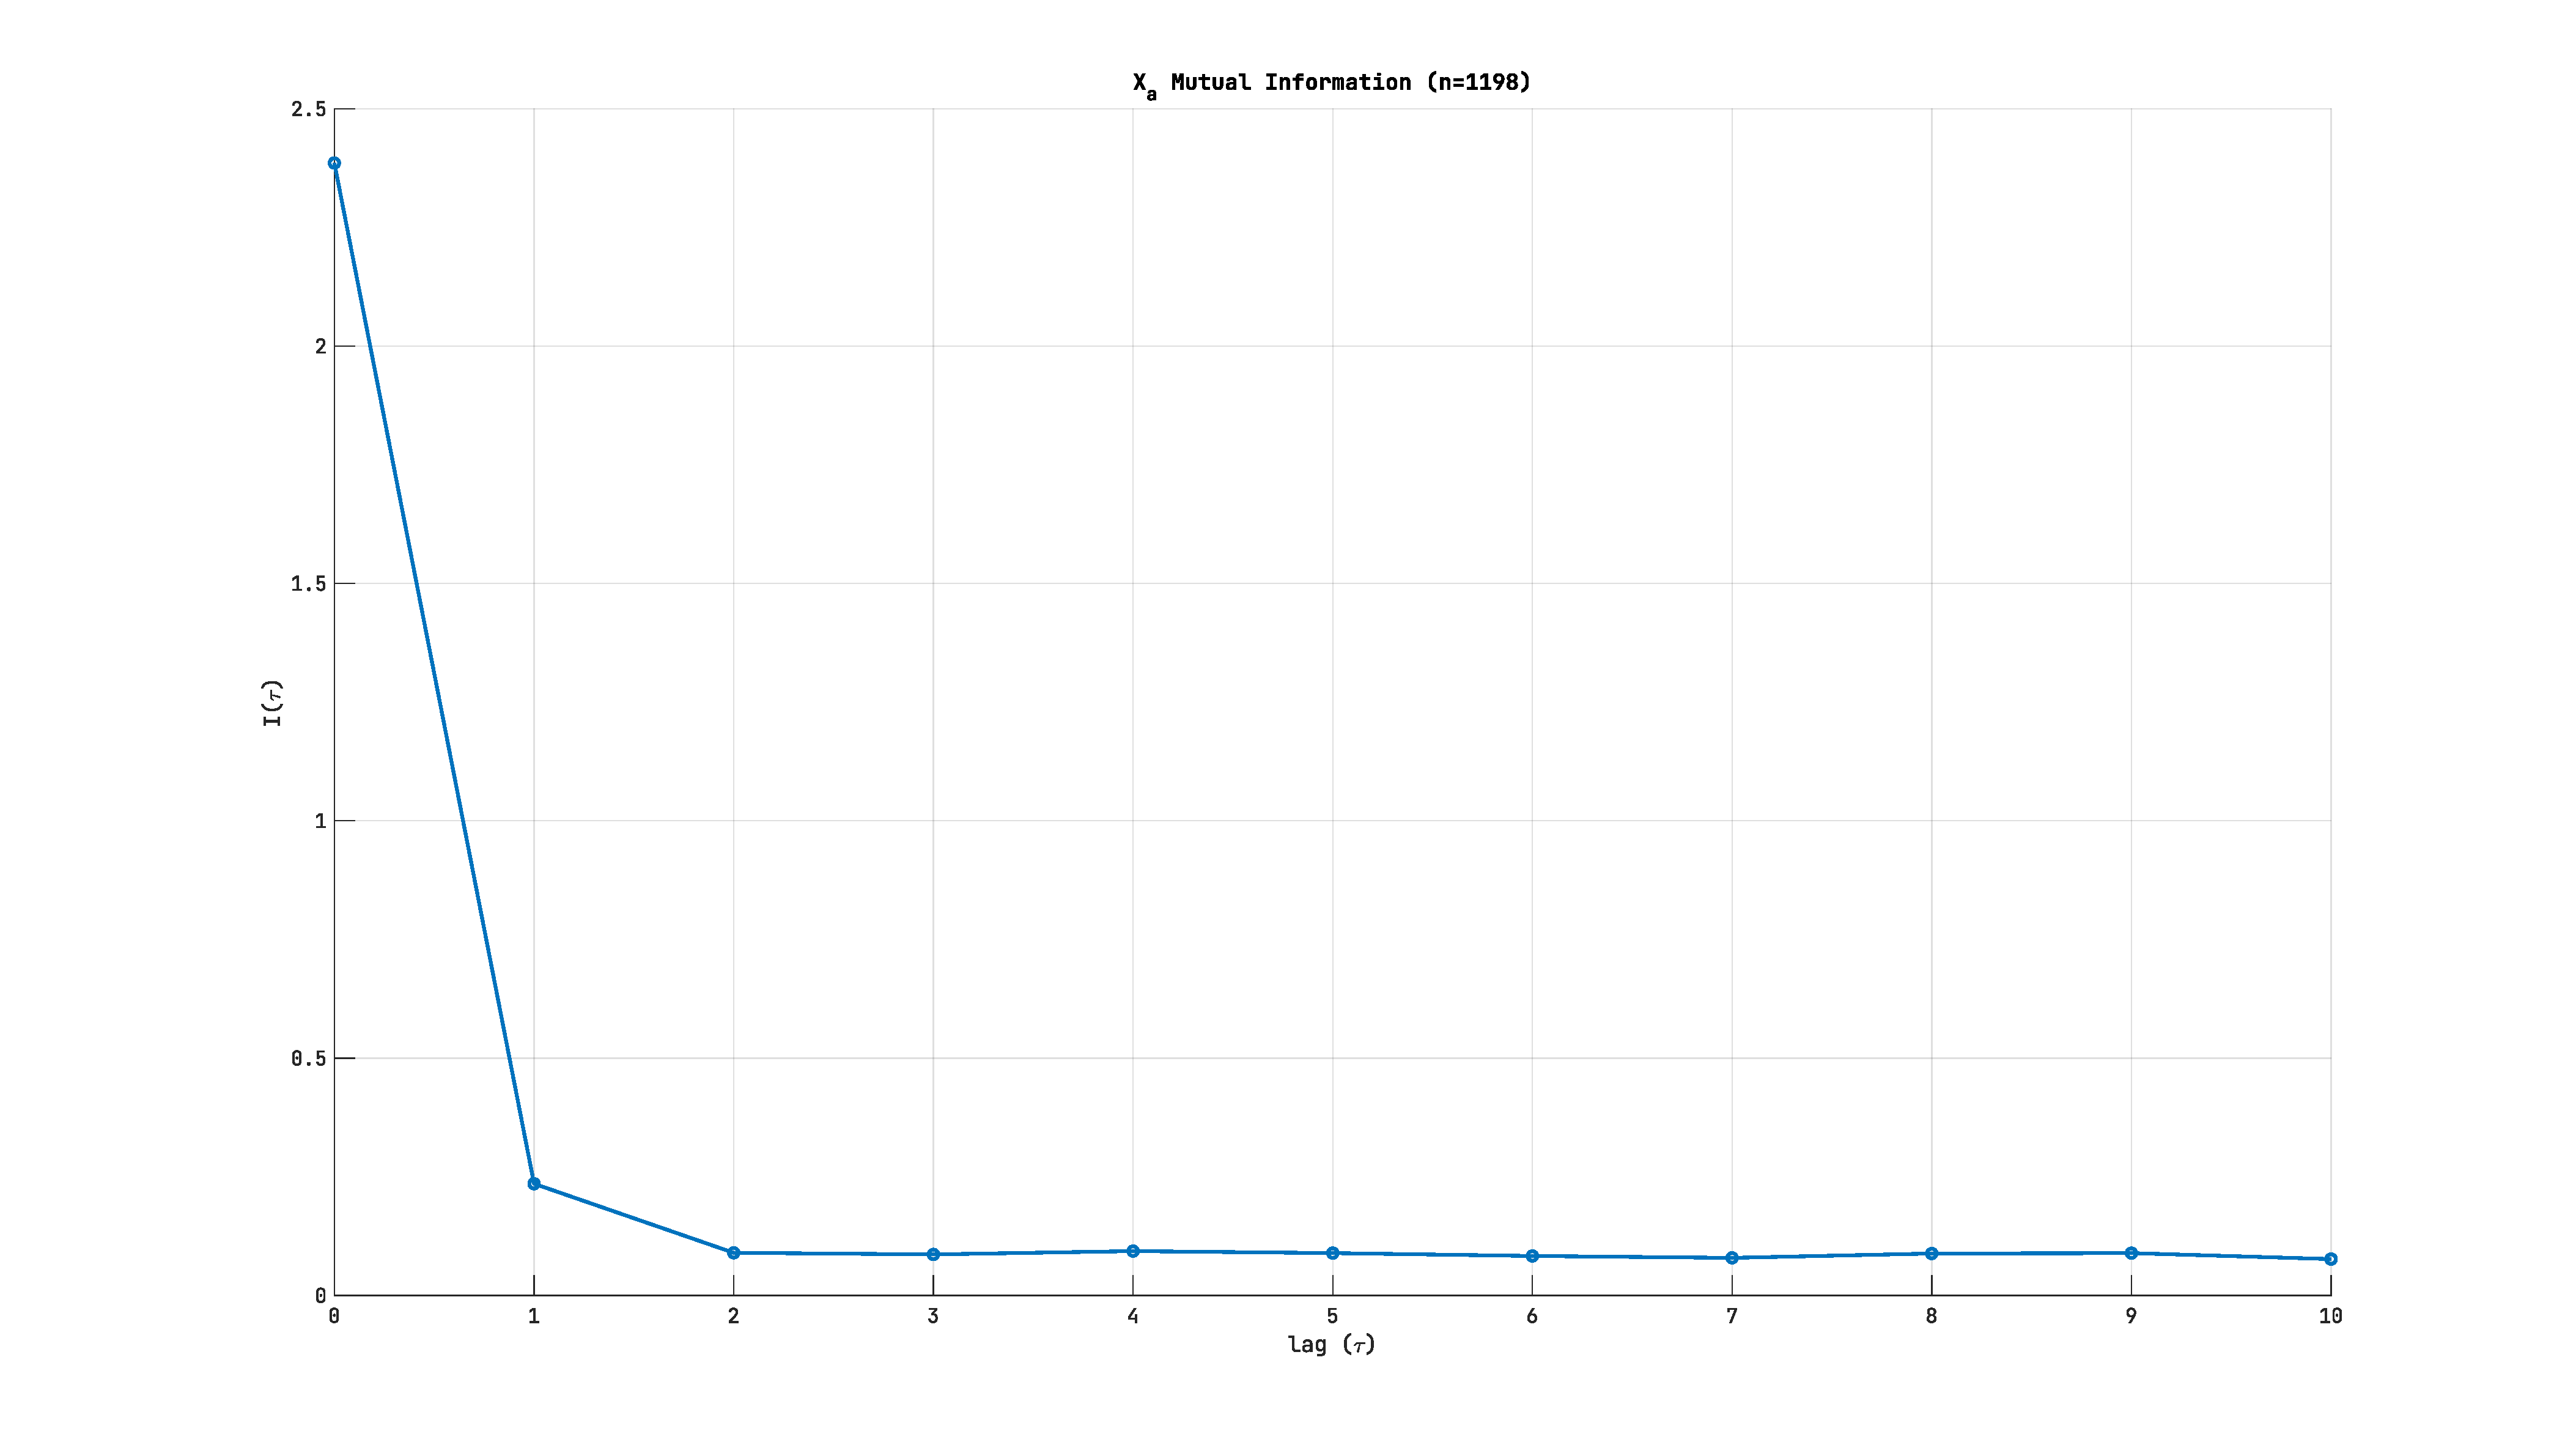
\includegraphics[width=\textwidth]{assets/images/plots/mutual_information_a.svg.pdf}
        \caption{Διάγραμμα αμοιβαίας πληροφορίας της στάσιμης χρονοσειράς $\{X_a(t)\}$ για επιλογή της υστέρησης $\tau$}
        \label{fig:mutual_information_a}
    \end{center}
\end{figure}

Βλέποντας λοιπόν ότι το πρώτο τοπικό ελάχιστο της $I(\tau)$ είναι για $\tau=3$ (θέλει αρκετό ζουμ - στη πράξη χρησιμοποιήθηκε η συνάρτηση \texttt{\tl{islocalmin()}} του \tl{MATLAB}), θα θεωρήσουμε για τη στάσιμη χρονοσειρά \tl{A} ότι \textbf{τ=3}.

\subsubsection{Διάσταση Εμβύθινσης Ελκυστή, \tl{m}}

Πριν αναζητήσουμε τη διάσταση εμβύθινσης με τη μέθοδο \tl{False Nearest Neighbors} θα δούμε το διάγραμμα διασποράς (\tl{scatter plot}) ώστε να διαπιστώσουμε εάν πρόκειται για χαμηλοδιάστατο ελκυστή. 

\begin{figure}[H]
    \begin{center}
        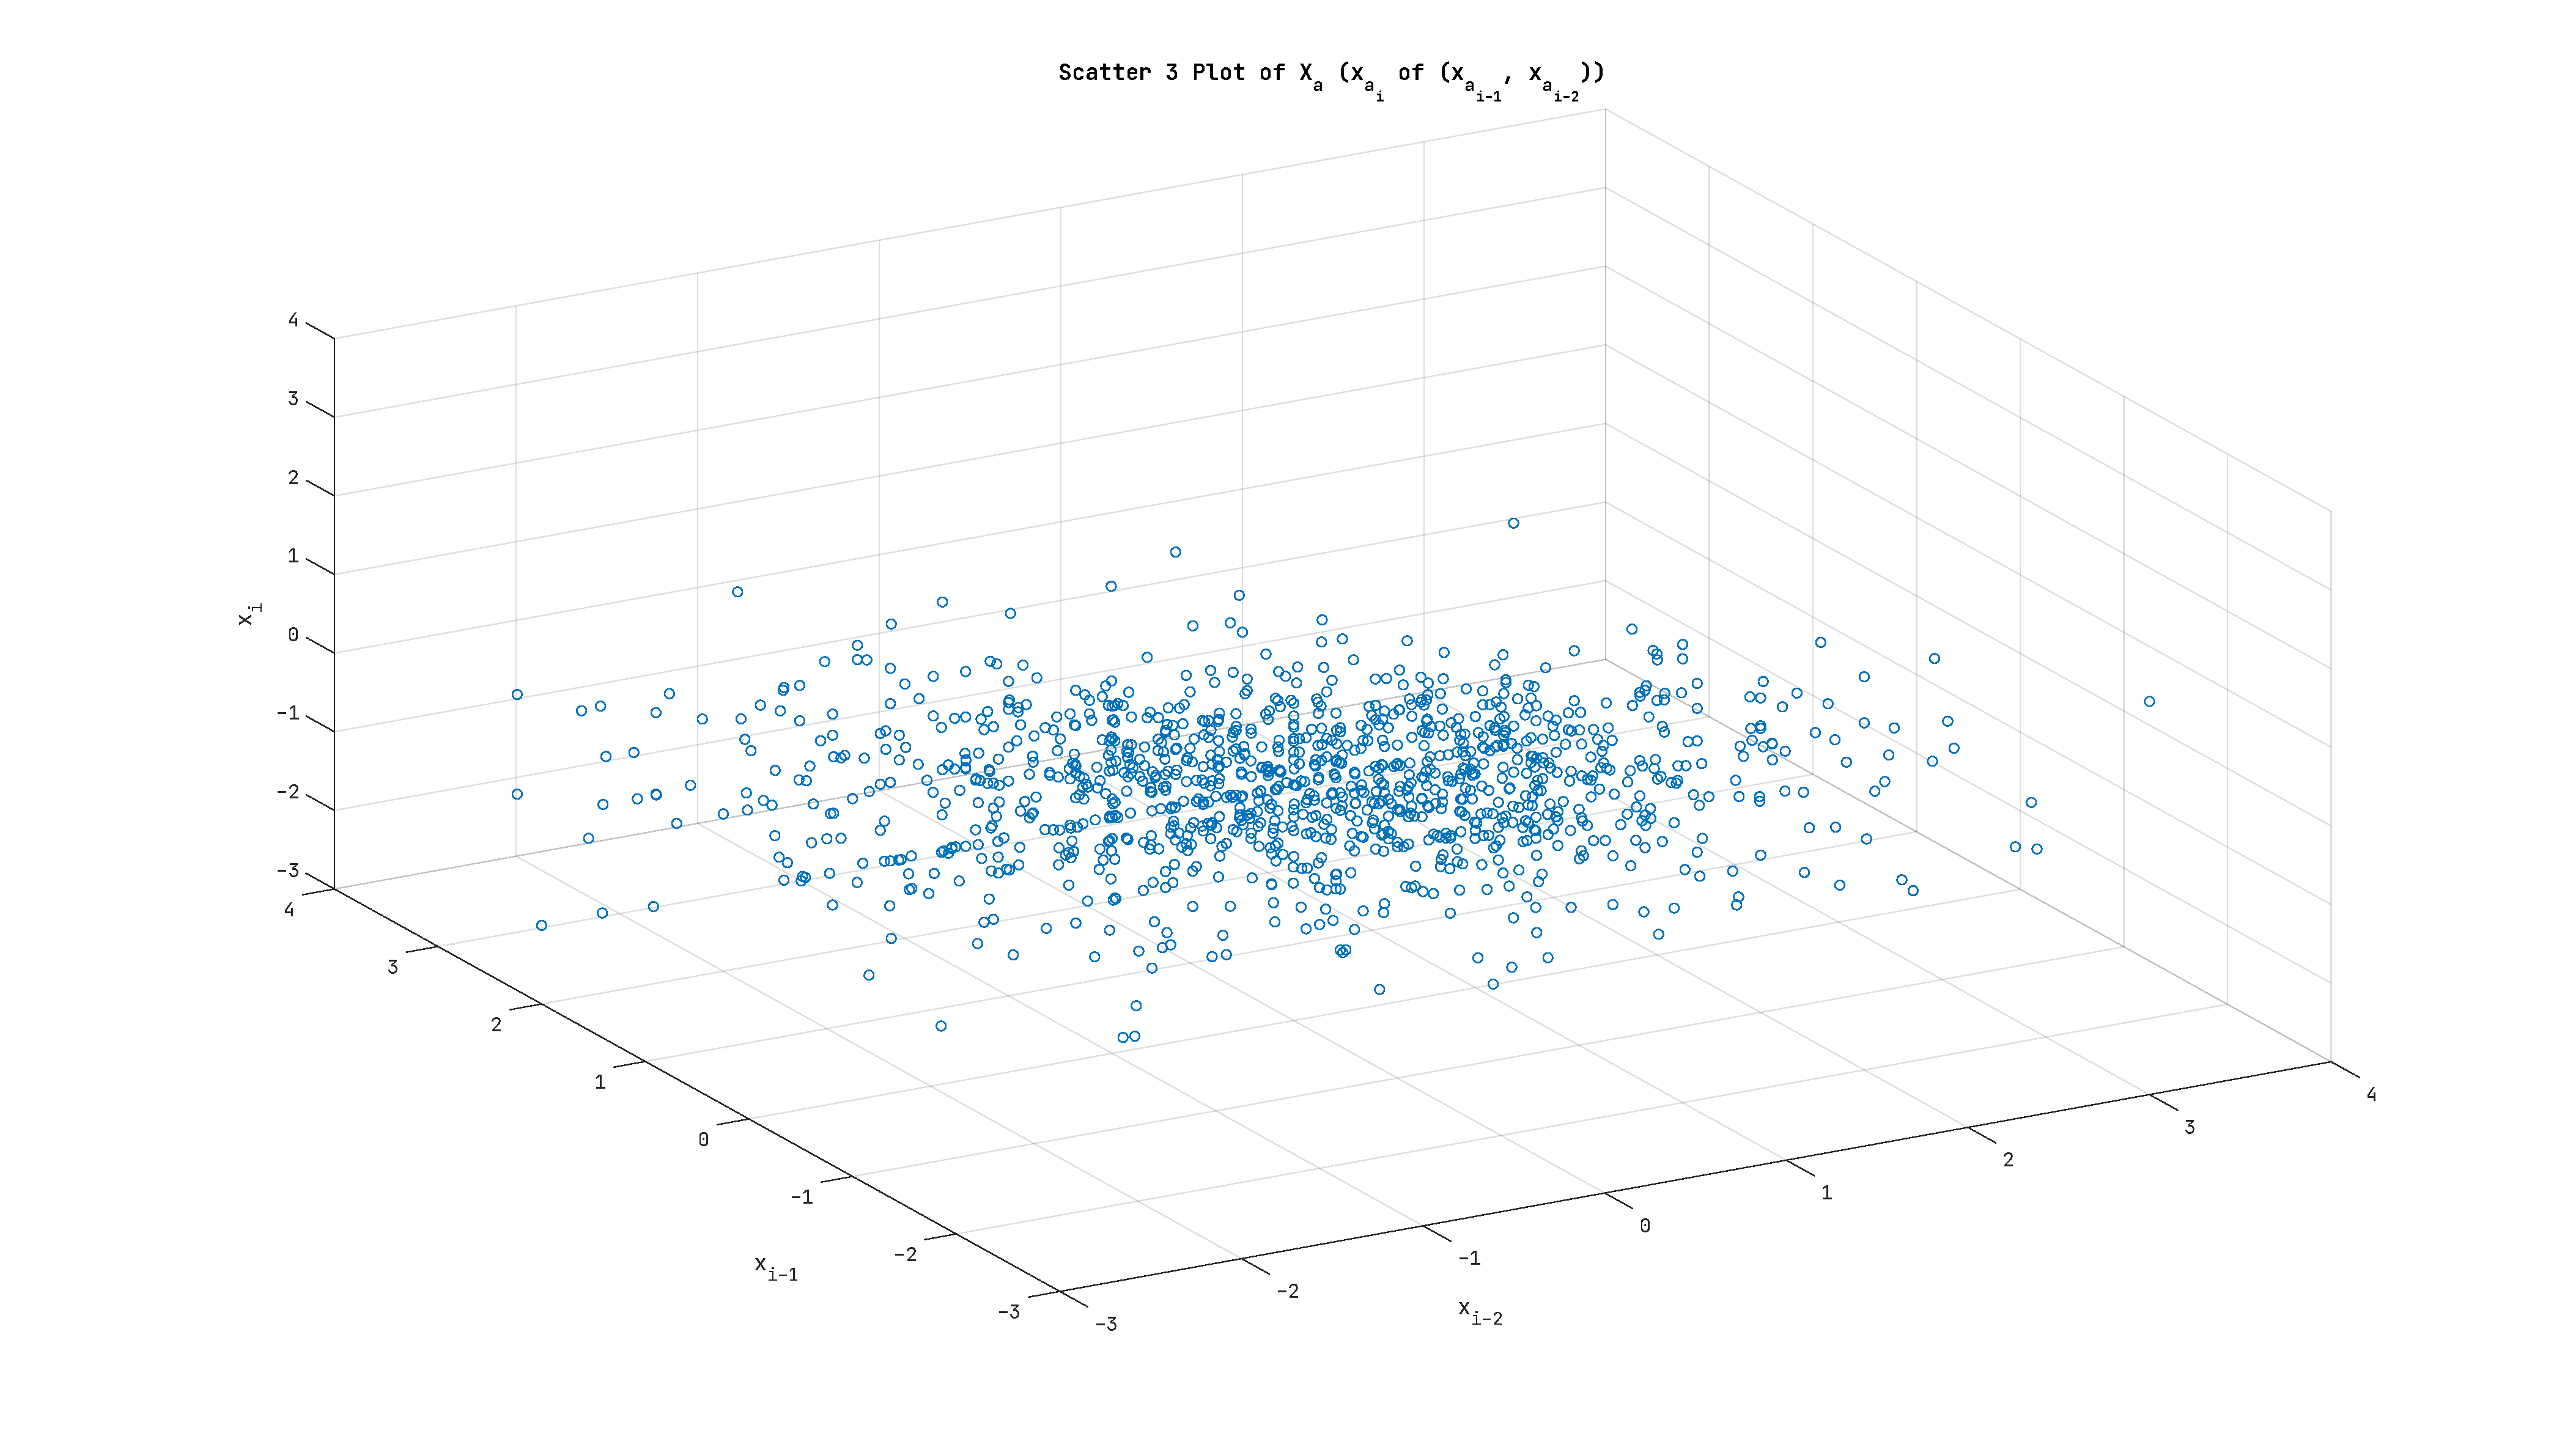
\includegraphics[width=\textwidth]{assets/images/plots/scatter3_a.svg.pdf}
        \caption{Διάγραμμα διασποράς $x_i-x_{i-1}-x_{i-2}$ της στάσιμης χρονοσειράς $\{X_a(t)\}$}
        \label{fig:scatter3_a}
    \end{center}
\end{figure}

Από το παραπάνω διάγραμμα (αν και φαίνεται κάποιο υποσύνολο των σημείων του διαγράμματος να έχει κάποια δομή - μια ευθεία γραμμή που ξεκινάει από το $x_{i-1}=3, x_{i}=-3$), δεν φαίνεται να υπάρχει κάποια δομή που να ακολουθούν όλα τα σημεία του \tl{scatter plot} και επομένως υποψιαζόμαστε ότι ο ελκυστής (εφόσον υπάρχει) θα βρίσκεται σε μεγαλύτερες διαστάσεις (π.χ. 4-\tl{D}, 5-\tl{D} κλπ).

\par Ακολούθως, τρέχουμε τη δοσμένη συνάρτηση \texttt{\tl{falsenearest()}} με παράμετρο \texttt{\tl{tau=3}} και από το διάγραμμα της μεταβολής των \tl{FNNs} θα καταλήξουμε στην κατάλληλη τιμή του $m$:

\begin{figure}[H]
    \begin{center}
        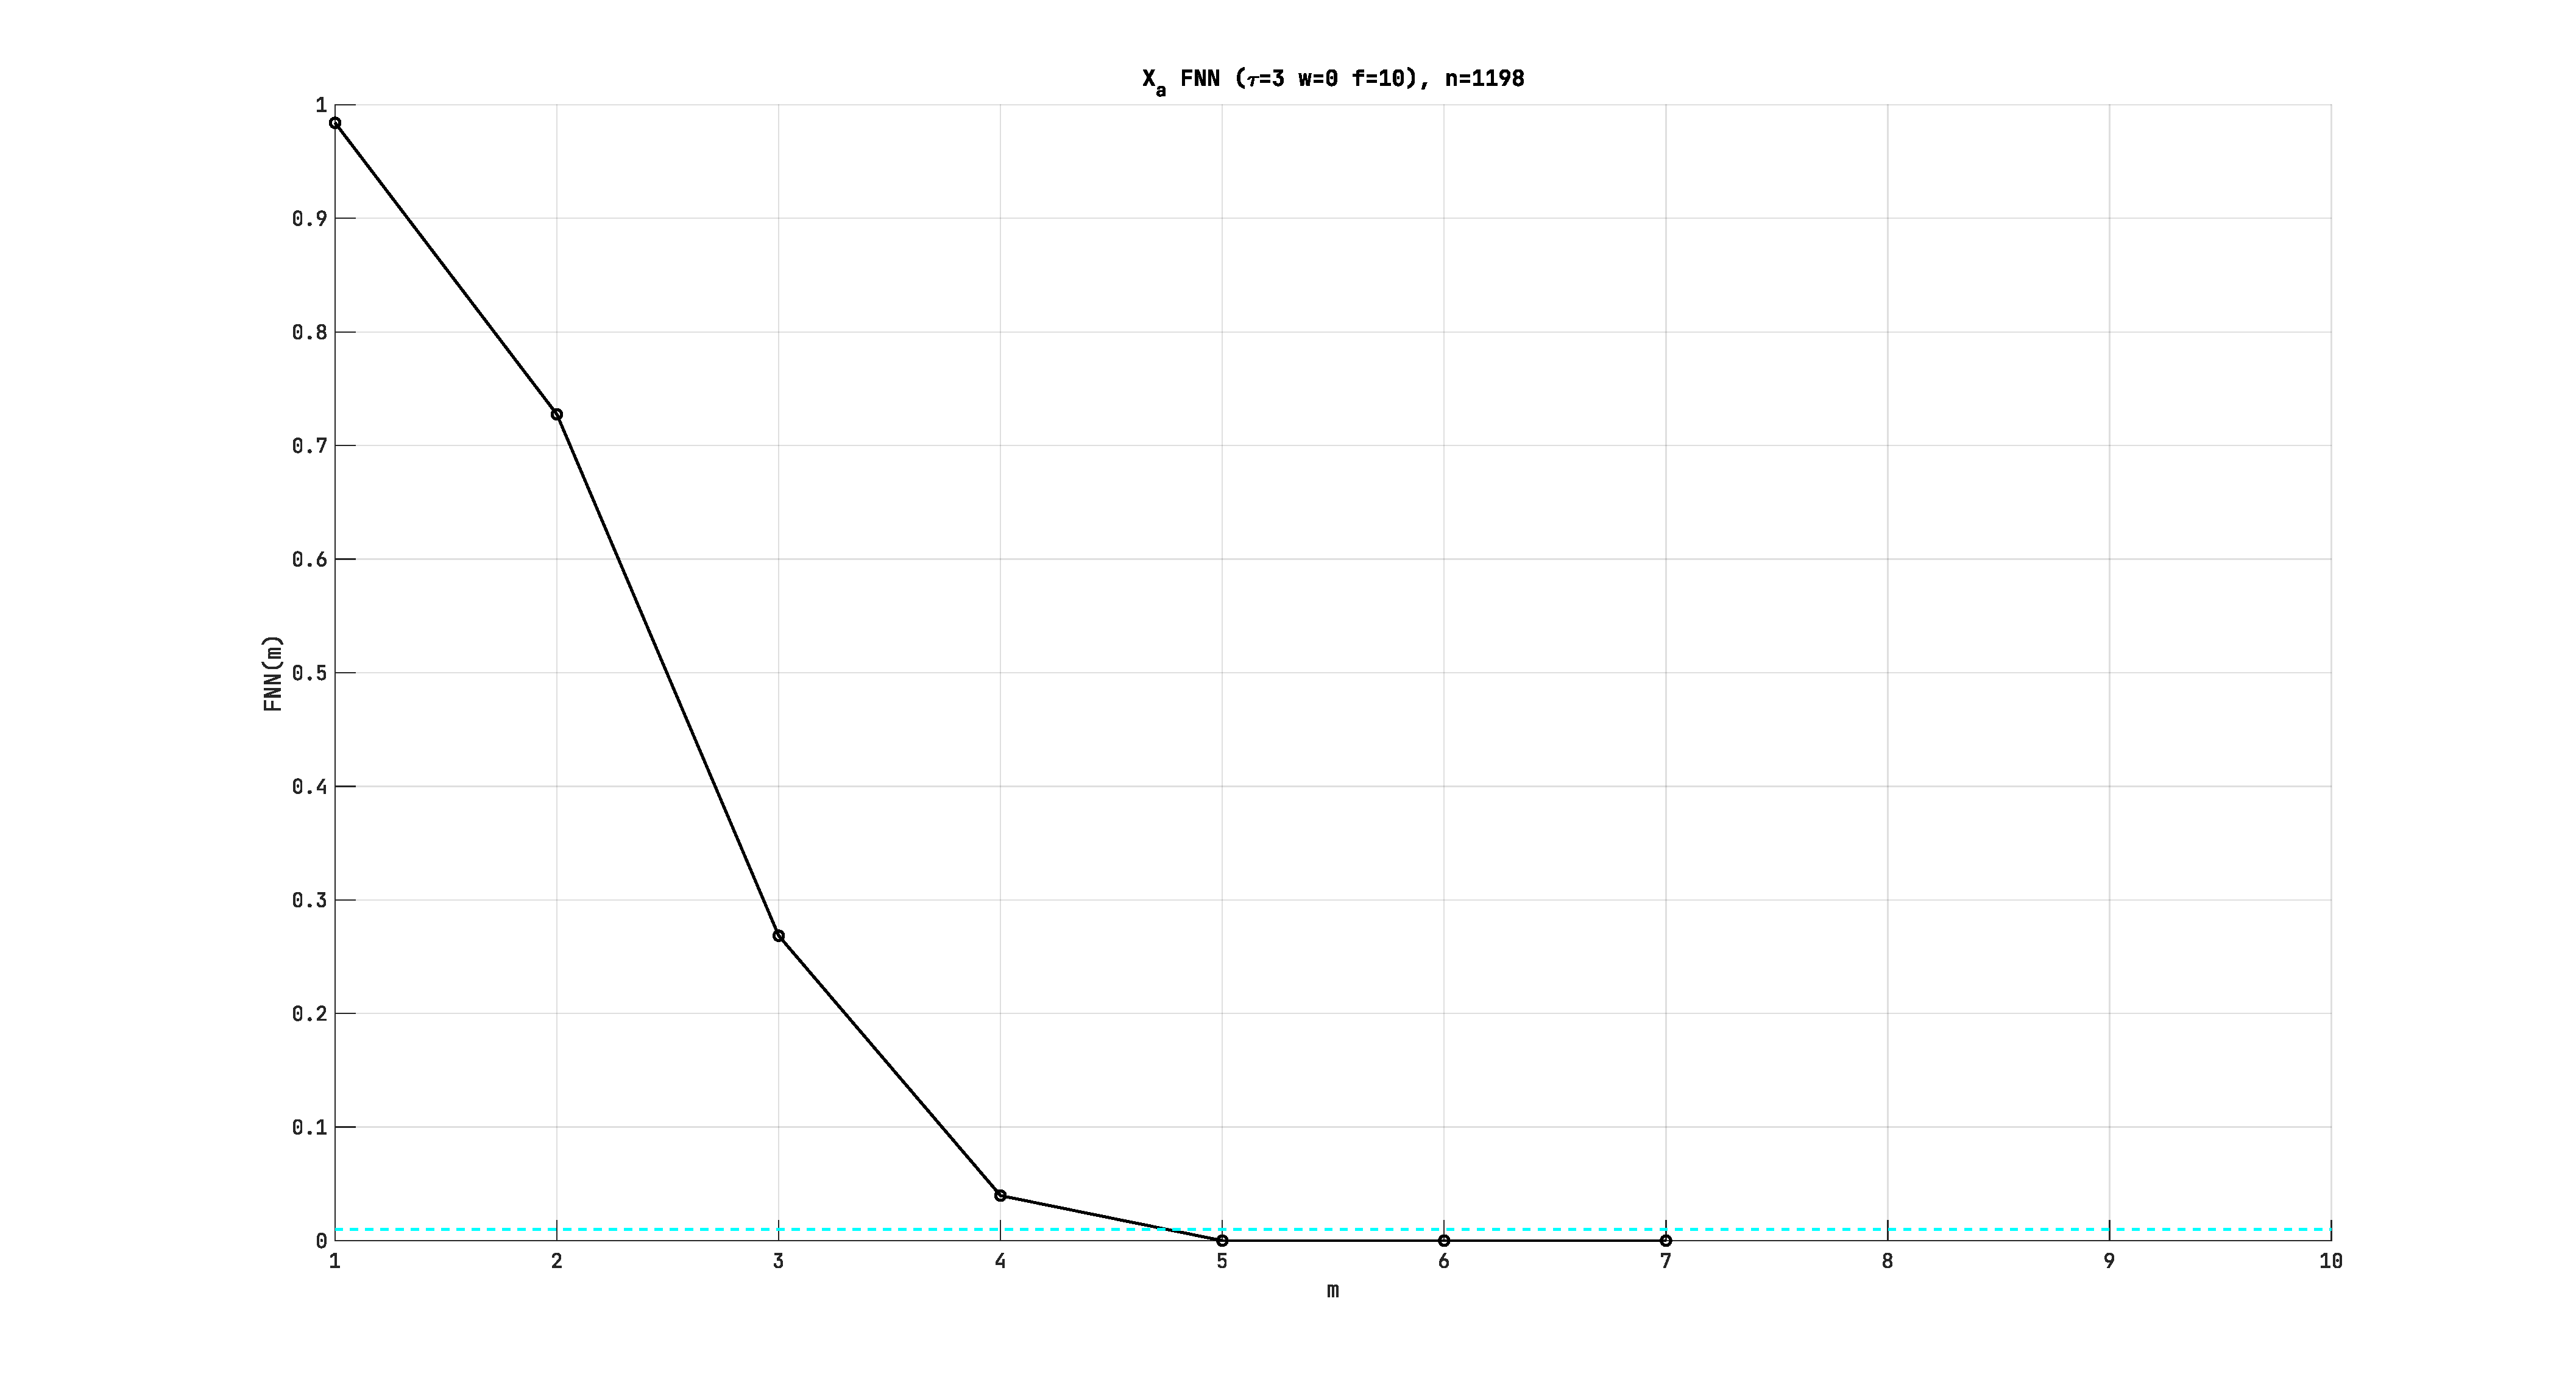
\includegraphics[width=\textwidth]{assets/images/plots/fnn_a.svg.pdf}
        \caption{Διάγραμμα μεταβολής των \tl{FNNs} ως προς τη διάσταση εμβύθινσης, $m$, για τη στάσιμη χρονοσειρά $\{X_a(t)\}$}
        \label{fig:fnn_a}
    \end{center}
\end{figure}

Στο παραπάνω διάγραμμα έχει σημειωθεί και το όριο επιλογής 1\%. Επιλέγουμε λοιπόν για διάσταση εμβύθινσης, \textbf{\tl{m=5}} για την στάσιμη χρονοσειρά \tl{A}. 

\par \textit{Σημειώνεται, πως για να τρέξει η παραπάνω συνάρτηση για όλες τις εκτελέσεις έπρεπε να μεγαλώσει η ακτίνα αναζήτησης ψευδών γειτόνων, από 0.1 που ήταν η προεπιλογή σε \texttt{\tl{fthres=0.3}}.}

\par Επομένως, τα σημεία του ανακατασκευασμένου χώρου καταστάσεων θα είναι τα εξής:
\begin{align}
    \mathbf{x}_{a_i} = \left[x_{a_i}, x_{a_{i-3}}, x_{a_{i-6}}, x_{a_{i-9}}, x_{i-12}\right] \in \mathbb{R}^5, \ \ \ i=13,...,1998
\end{align}

\subsection{Παράμετροι ανακατασκευής για τη Χρονοσειρά \tl{B}}

\subsubsection{Υστέρηση, τ}

Αντίστοιχα με τη χρονοσειρά \tl{A}, για την εύρεση της υστέρησης στη δεύτερη (στάσιμη) χρονοσειρά, δίνεται το διάγραμμα της αμοιβαίας πληροφορίας, $I_b(\tau)$, και παραθέτεται η επιλεγμένη τιμή για την υστέρηση.

\begin{figure}[H]
    \begin{center}
        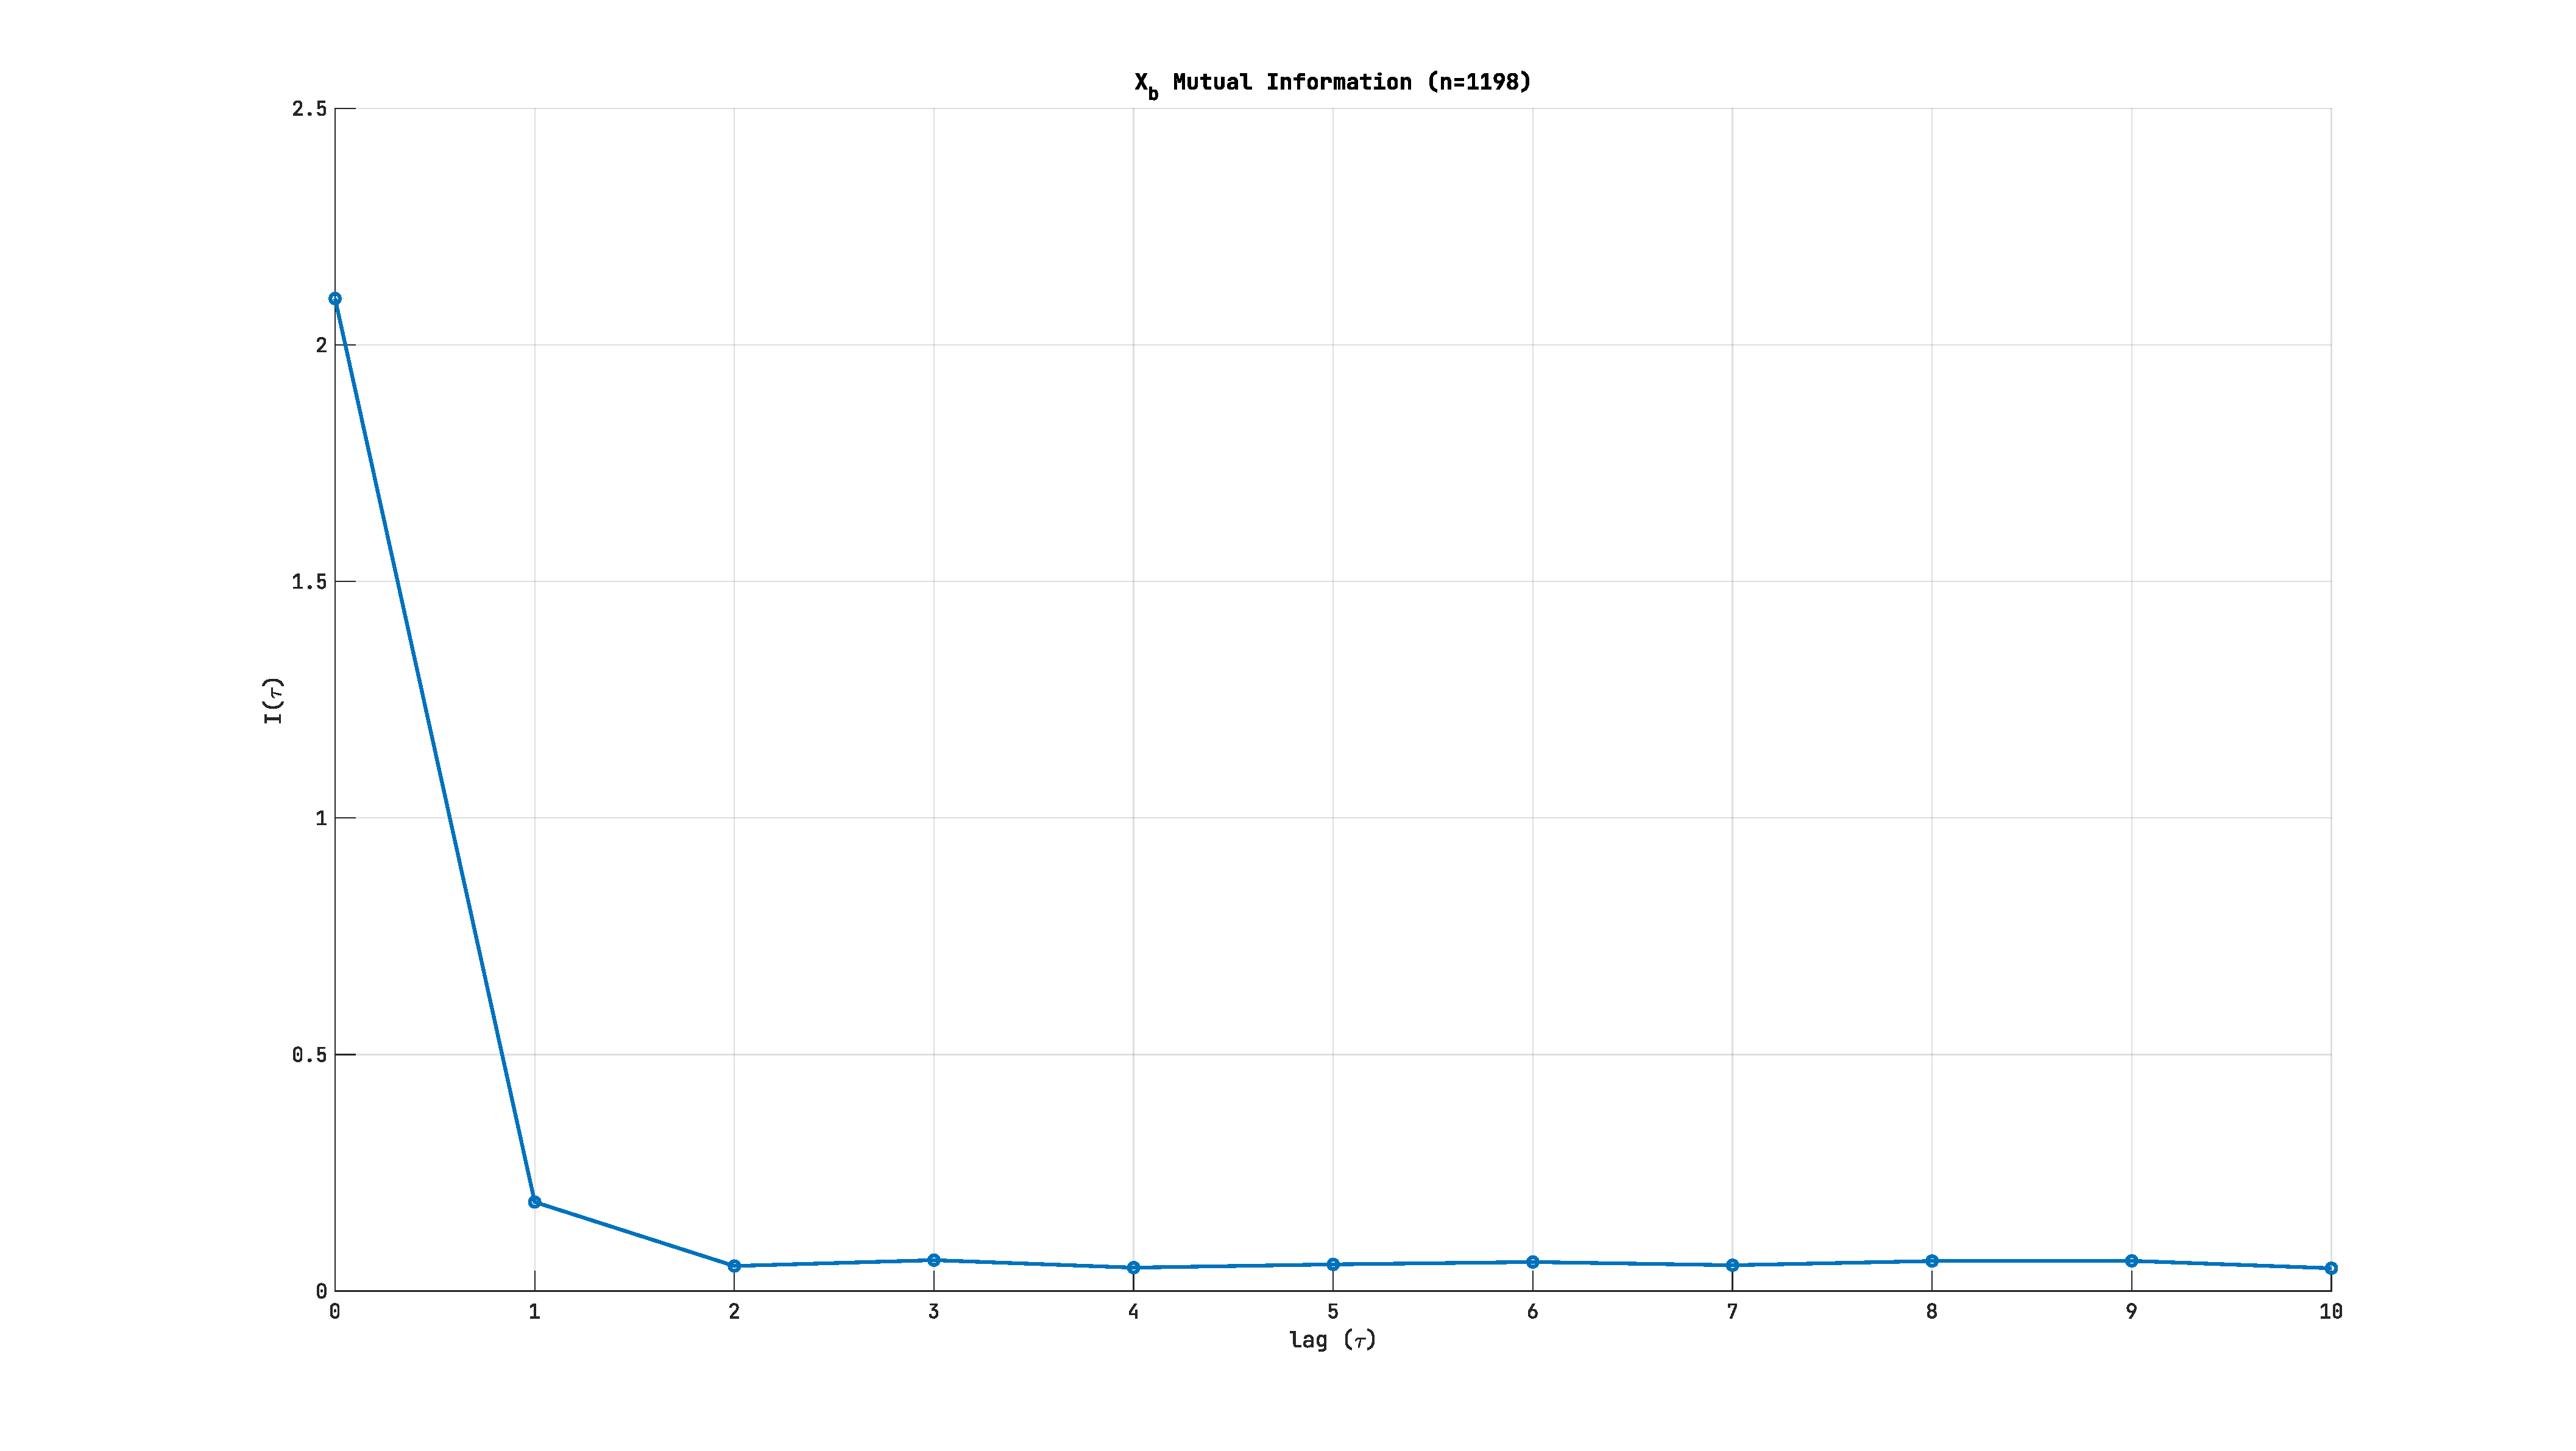
\includegraphics[width=\textwidth]{assets/images/plots/mutual_information_b.svg.pdf}
        \caption{Διάγραμμα αμοιβαίας πληροφορίας της στάσιμης χρονοσειράς $\{X_{b_{deseasoned}}(t)\}$ για επιλογή της υστέρησης $\tau$}
        \label{fig:mutual_information_b}
    \end{center}
\end{figure}

Βλέποντας στο παραπάνω διάγραμμα ότι το πρώτο τοπικό ελάχιστο της $I(\tau)$ είναι για $\tau=2$ θα θεωρήσουμε για τη στάσιμη χρονοσειρά \tl{B} ότι \textbf{τ=2}.

\subsubsection{Διάσταση Εμβύθινσης Ελκυστή, \tl{m}}

Πριν αναζητήσουμε τη διάσταση εμβύθινσης με τη μέθοδο \tl{False Nearest Neighbors} θα δούμε το διάγραμμα διασποράς (\tl{scatter plot}) ώστε να διαπιστώσουμε εάν πρόκειται για χαμηλοδιάστατο ελκυστή. 

\begin{figure}[H]
    \begin{center}
        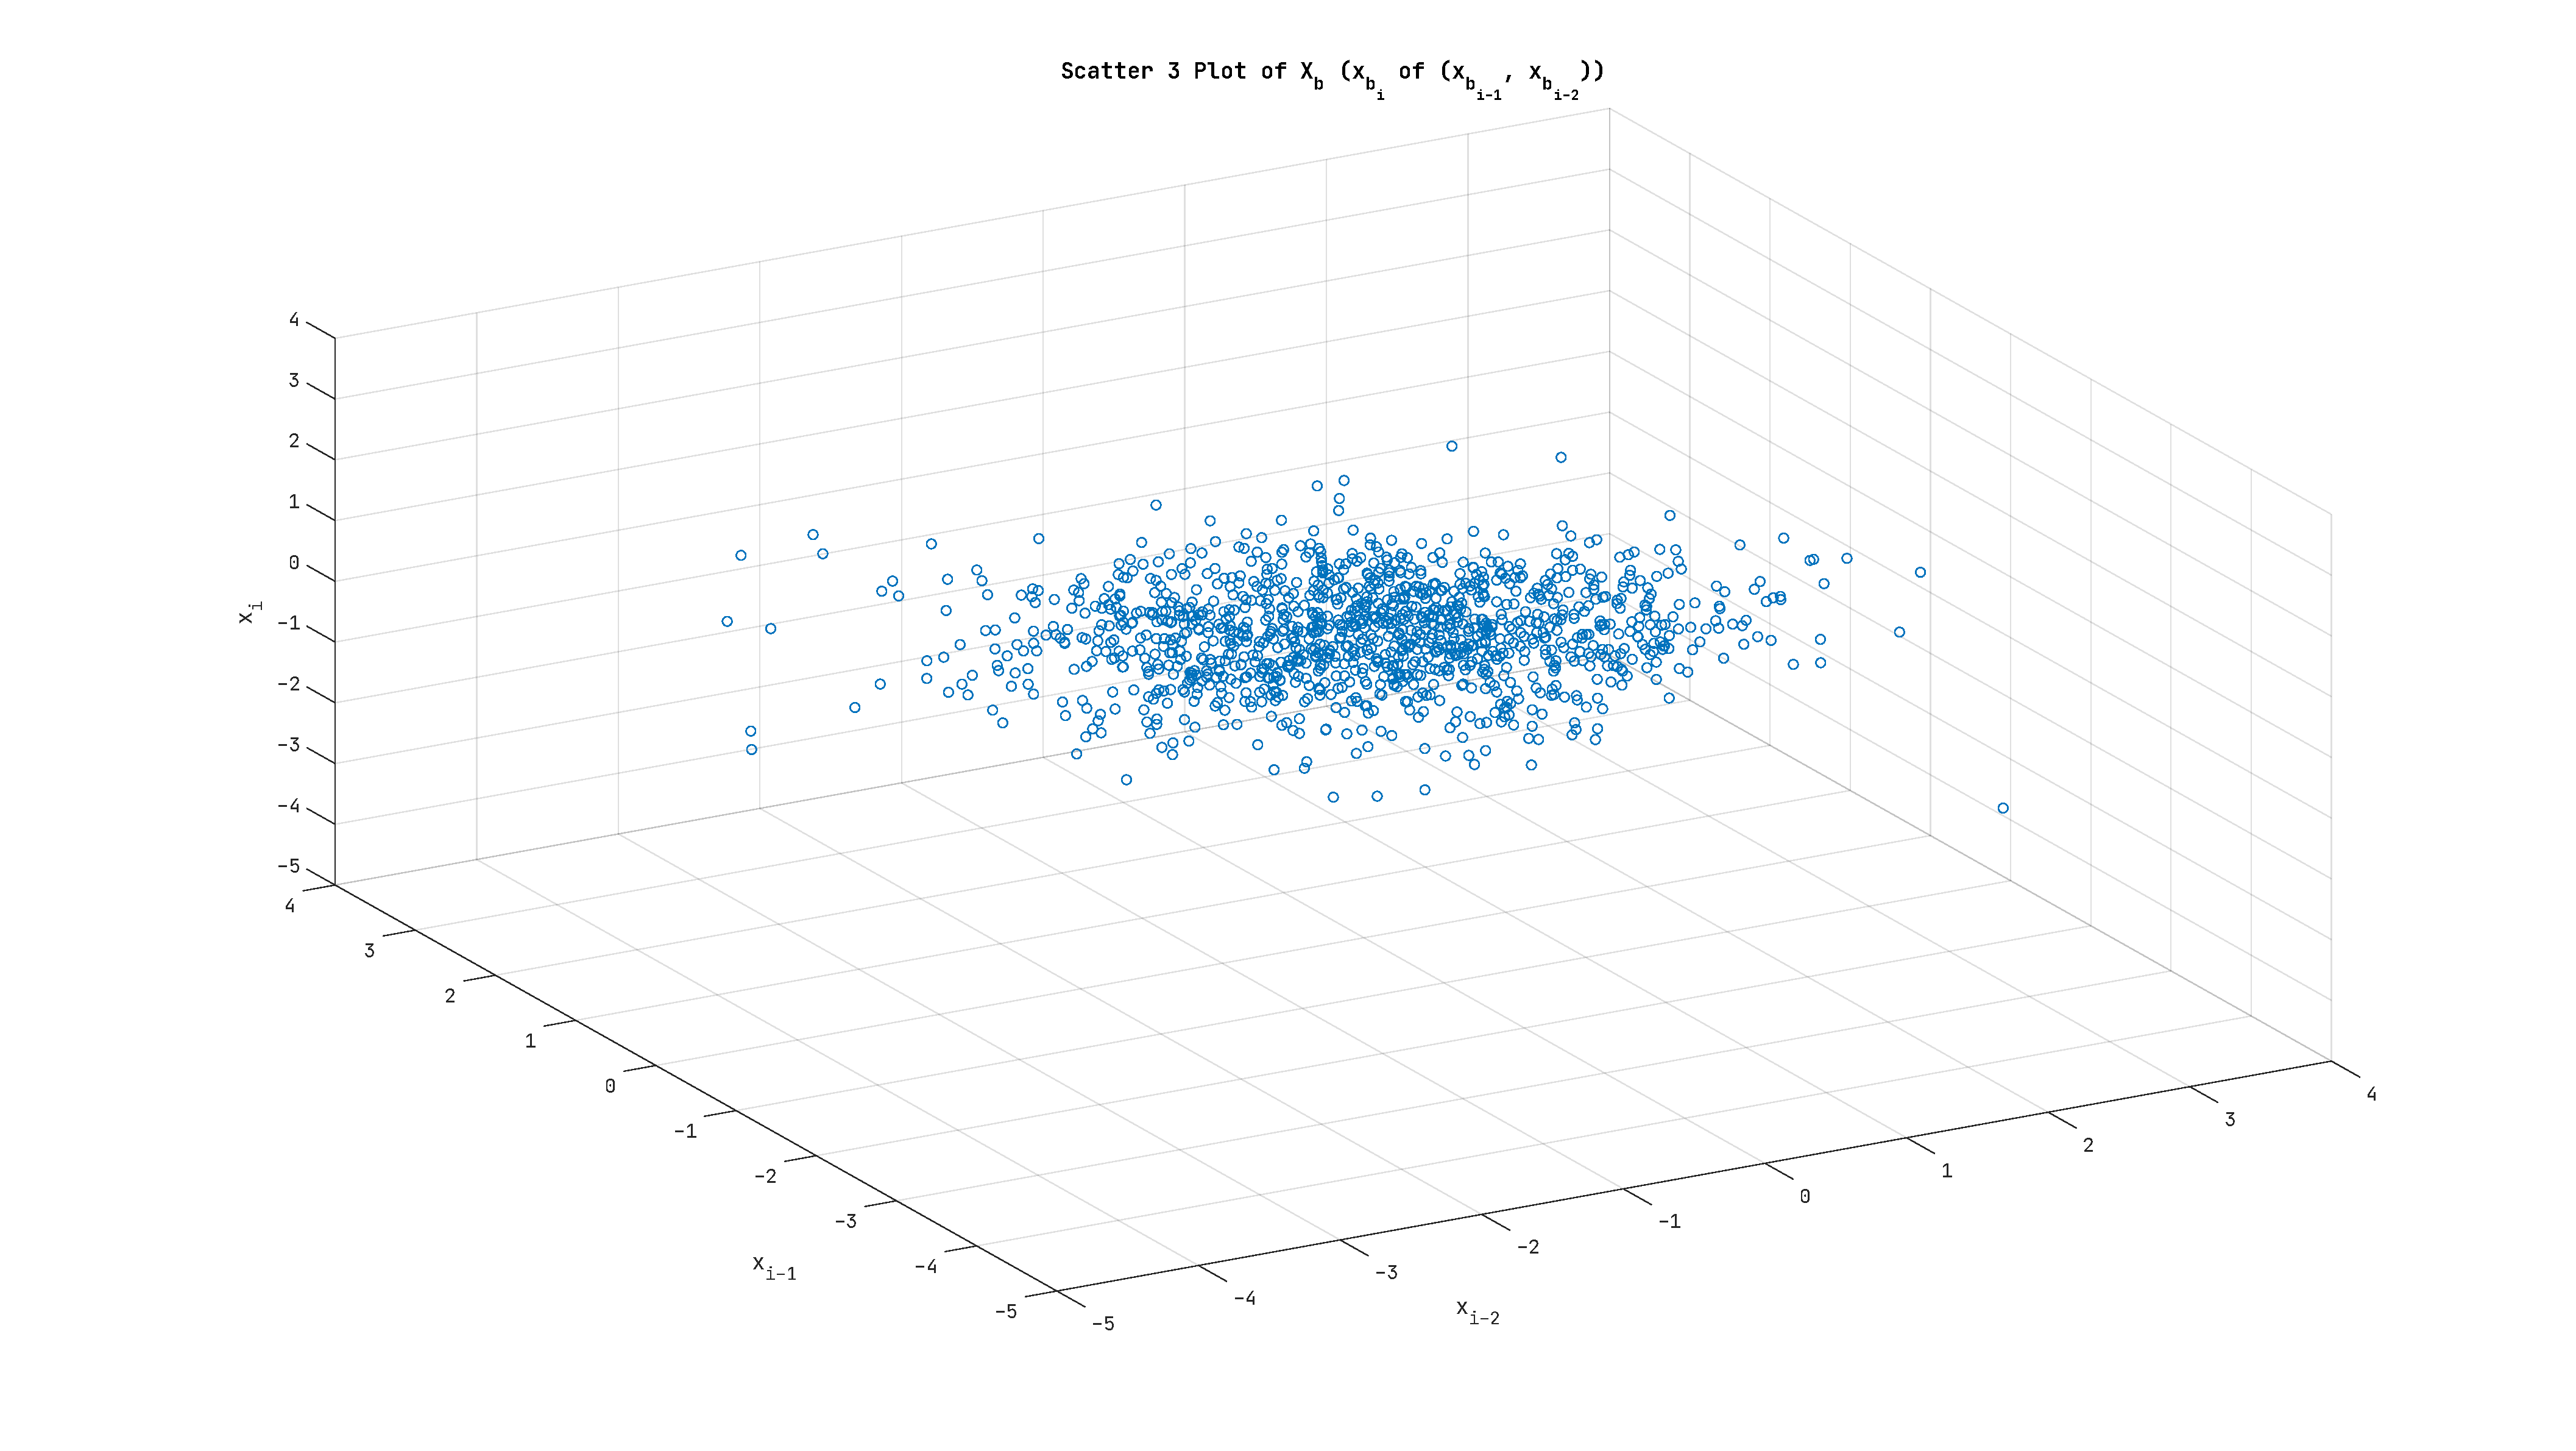
\includegraphics[width=\textwidth]{assets/images/plots/scatter3_b.svg.pdf}
        \caption{Διάγραμμα διασποράς $x_i-x_{i-1}-x_{i-2}$ της στάσιμης χρονοσειράς $\{X_{b_{deseasoned}}(t)\}$}
        \label{fig:scatter3_b}
    \end{center}
\end{figure}

Από το παραπάνω διάγραμμα δεν φαίνεται να υπάρχει καμία δομή που να ακολουθούν όλα τα σημεία του \tl{scatter plot} και επομένως υποψιαζόμαστε ότι ο ελκυστής (εφόσον υπάρχει) θα βρίσκεται σε μεγαλύτερες διαστάσεις (π.χ. 4-\tl{D}, 5-\tl{D} κλπ). Τα σημεία του \tl{scatter plot} φαίνονται συγκεντρωμένα σε μία άμορφη περιοχή του τρισδιάστατου χώρου.

\par Ακολούθως, τρέχουμε τη δοσμένη συνάρτηση \texttt{\tl{falsenearest()}} με παράμετρο \texttt{\tl{tau=2}} και από το διάγραμμα της μεταβολής των \tl{FNNs} θα καταλήξουμε στην κατάλληλη τιμή του $m$:

\begin{figure}[H]
    \begin{center}
        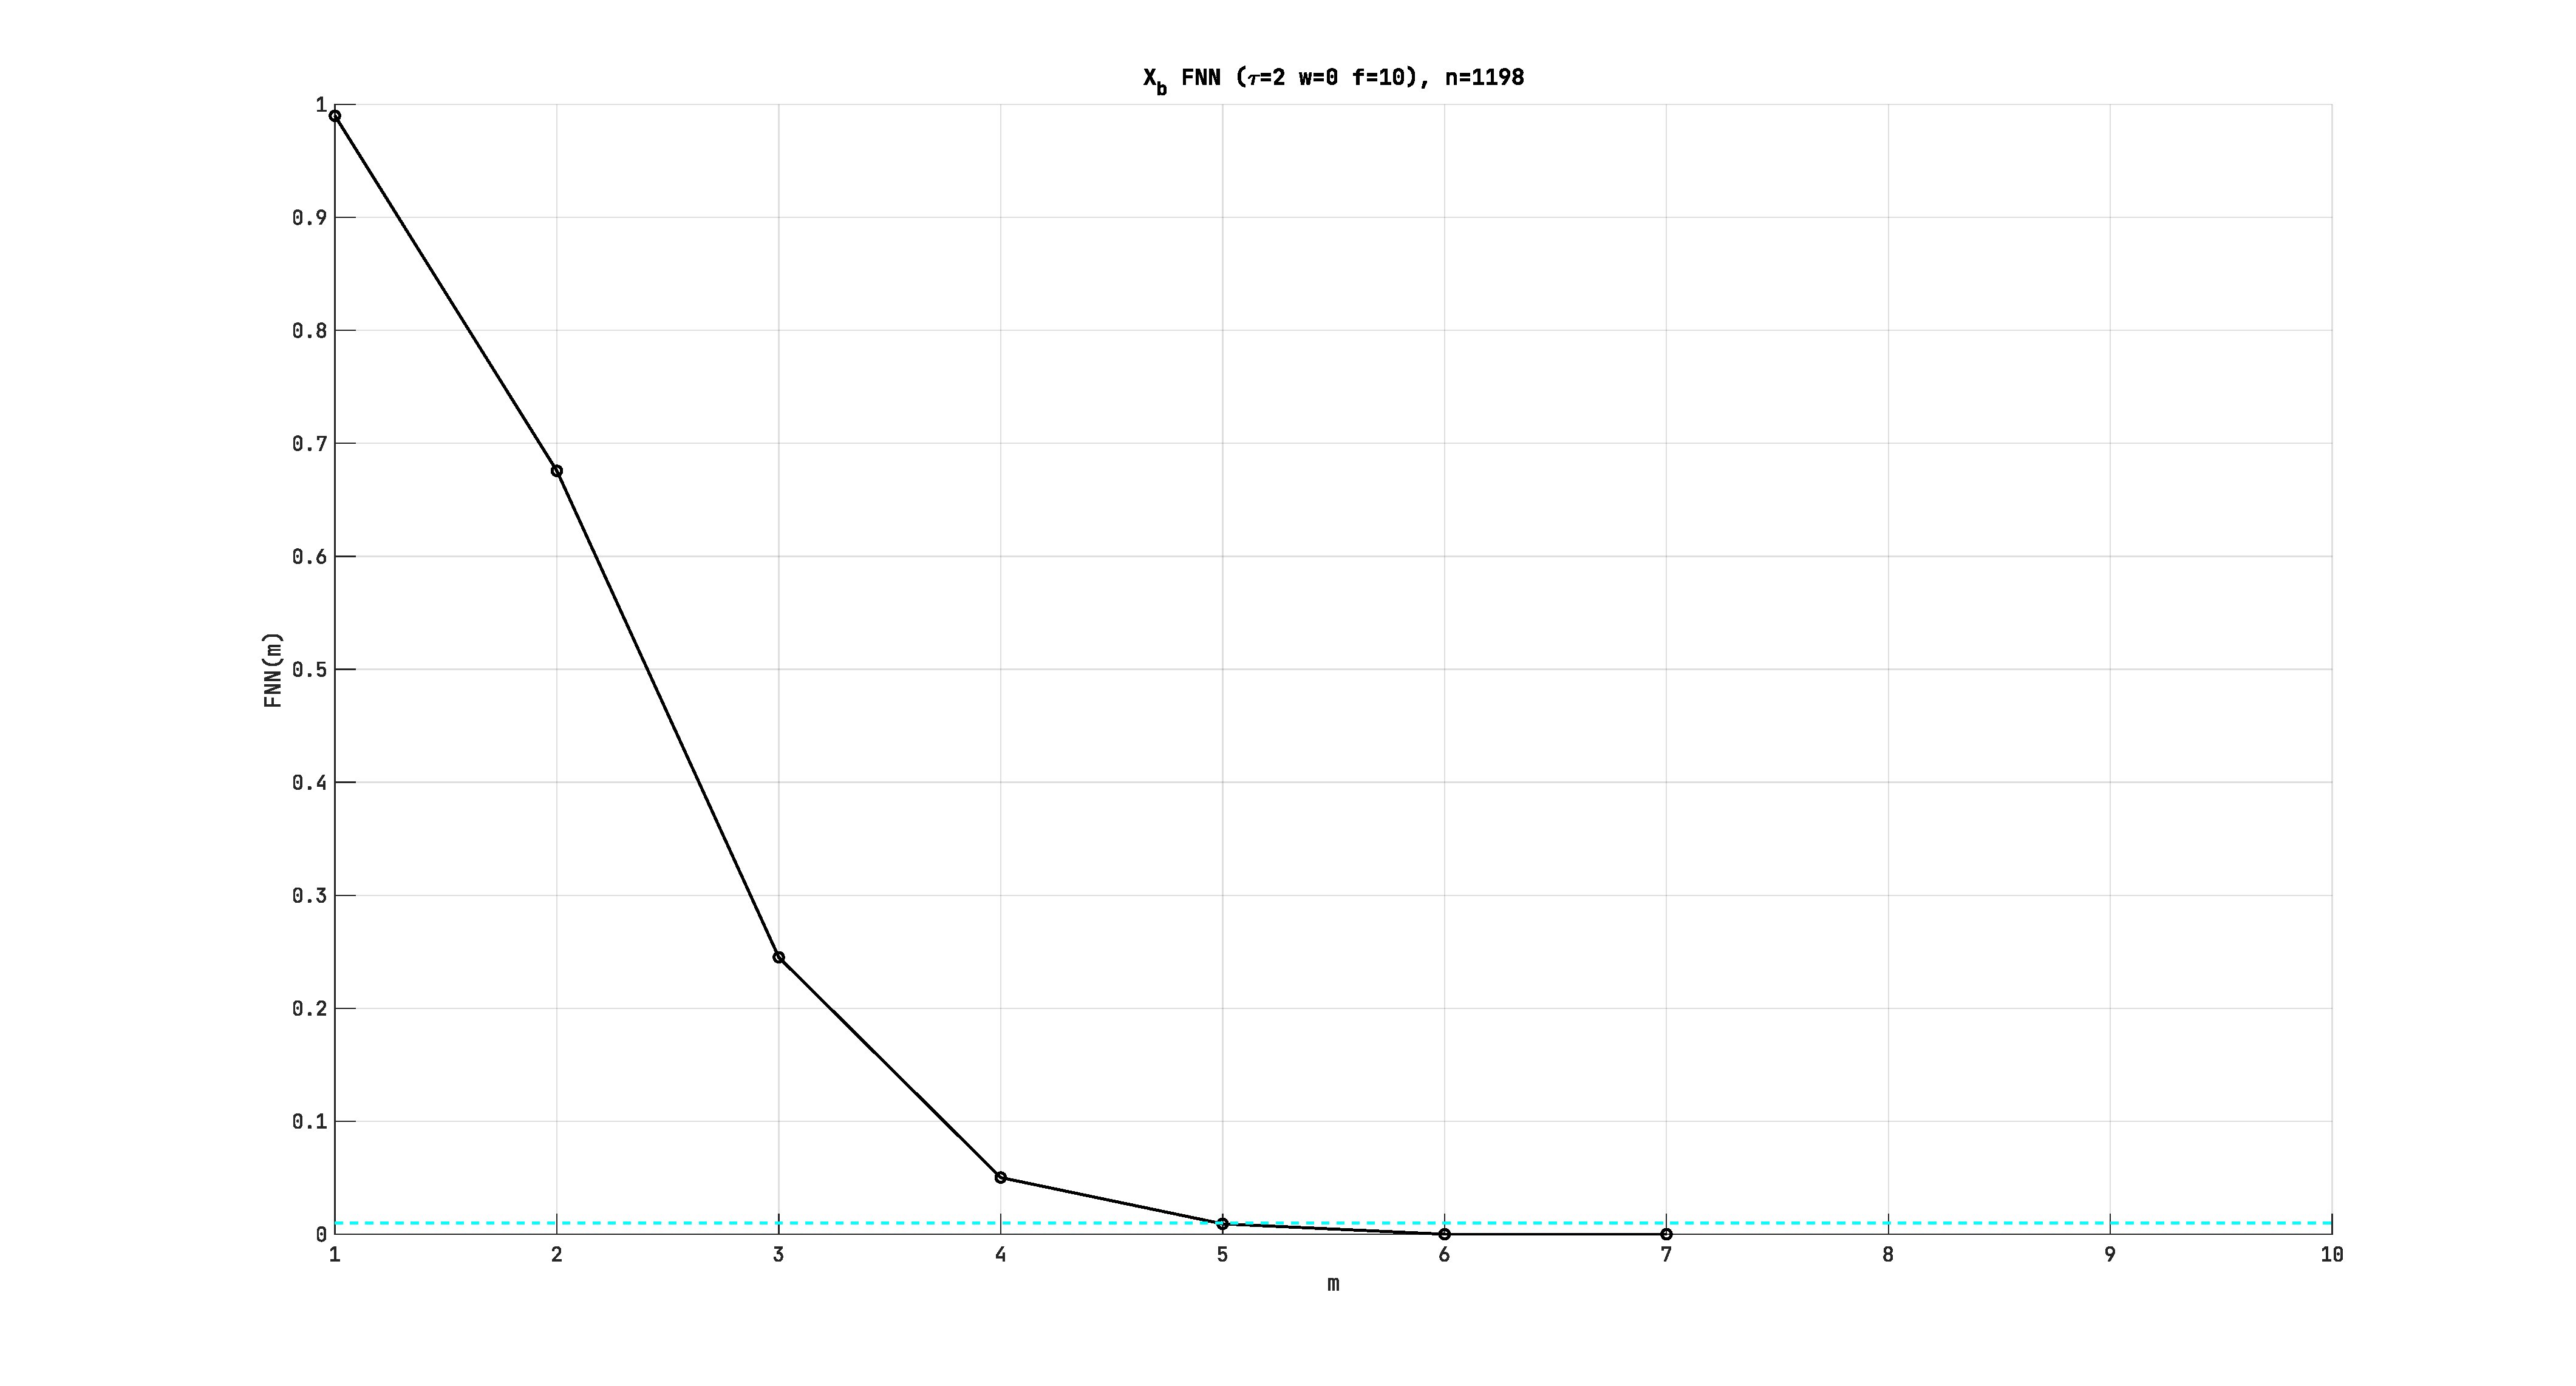
\includegraphics[width=\textwidth]{assets/images/plots/fnn_b.svg.pdf}
        \caption{Διάγραμμα μεταβολής των \tl{FNNs} ως προς τη διάσταση εμβύθινσης, $m$, για τη στάσιμη χρονοσειρά $\{X_{b_{deseasoned}}(t)\}$}
        \label{fig:fnn_b}
    \end{center}
\end{figure}

Η πρώτη τιμή που πέφτει κάτω από σημειωμένο όριο του 1\% είναι και εδώ το 5. Επιλέγουμε λοιπόν για διάσταση εμβύθινσης, \textbf{\tl{m=5}} για την στάσιμη χρονοσειρά \tl{B}.

\par Επομένως, τα σημεία του ανακατασκευασμένου χώρου καταστάσεων θα είναι τα εξής:
\begin{align}
    \mathbf{x}_{b_i} = \left[x_{b_i}, x_{b_{i-2}}, x_{b_{i-4}}, x_{b_{i-6}}, x_{i-8}\right] \in \mathbb{R}^5, \ \ \ i=9,...,1998
\end{align}


\section{Προσαρμογή Τοπικού Μοντέλου Κοντινότερων Γειτόνων}

Για τη πρόβλεψη με μη-γραμμικά μοντέλα θα χρησιμοποιηθεί τοπική πρόβλεψη μέσου όρου, όπου για ένα βήμα εμπρός προβλέψη ορίζεται ως εξής (σχέση 107 - σελ. 100):
\begin{align}
    x_i(1) = \frac{1}{K} \sum_{j=1}^{K} \mathbf{x}_{i(j) + 1}
    \label{eq:x_i_1_knn}
\end{align}
όπου $x_i(1)$ είναι η πρόβλεψη του μοντέλου για το (\tl{i}+1)-οστή παρατήρηση της στάσιμης χρονοσειράς, $x_{i+1}$, ενώ $\mathbf{x}_{i(k)}$ είναι ο \tl{k}-οστός κοντινότερος γείτονας του σημείου $\mathbf{x}_i$ στον ανακατσκευασμένο χώρο καταστάσεων. 

\par Το μόνο που πρέπει να τεθεί πριν γίνει εφαρμογή του μοντέλου τοπικού μέσου όρου για πρόβλεψη των στάσιμων χρονοσειρών, είναι ο αριθμός των κοντινοτερών γειτόνων, $K$. Ακολουθεί ανάλυση για την επιλογή της κατάλληλης τιμής του $K$ για κάθε μία από τις στάσιμες χρονοσειρές που καταλήξαμε στα βήματα \ref{ch:step2} και \ref{ch:step3} αντίστοιχα.

\subsection{Επιλογή του \tl{K} για τη στάσιμη χρονοσειρά \tl{A}}

Θα χρησιμοποιήσουμε την δοθείσα συνάρτηση \texttt{\tl{localpredictmultistep}()} για να κάνουμε προβλέψεις έως και $T$ βήματα εμπρός με παραμέτρους:
\begin{itemize}
    \item \textit{Ορίζοντας Πρόβλεψης, Τ}: Θα χρησιμοποίσουμε την βέλτιστη τιμή που καταλήξαμε στο βήμα \ref{ch:step4}, δηλαδή $T=6$
    \item \textit{Διάσταση Εμβύθινσης, \tl{m}}: Θα χρησιμοποιήσουμε την τιμή που βρέθηκε από τη μέθοδο \tl{FNNs} εφαρμοζόμενη σε όλη τη στάσιμη χρονοσειρά Α, δηλαδή $m=5$
    \item \textit{Υστέρηση, τ}: Θα χρησιμοποιήσουμε την τιμή που βρέθηκε από τη συνάρτηση αμοιβαίας πληροφορίας ολόκληρης της στάσιμης χρονοσειράς Α, δηλαδή $\tau=3$
\end{itemize}

Παρακάτω εκτελούμε την συνάρτηση \texttt{\tl{localpredictmultistep}()}  για κάθε χρονική στιγμή με ορίσματα τις παραπάνω παραμέτρους καθώς και το $K=1,...,40$. Πλοτάρουμε το \tl{NRMSE} των σφαλμάτων πρόβλεψης και με βάση αυτό επιλέγουμε την καταλληλότερη τιμή για το $K$.

\begin{figure}[H]
    \begin{center}
        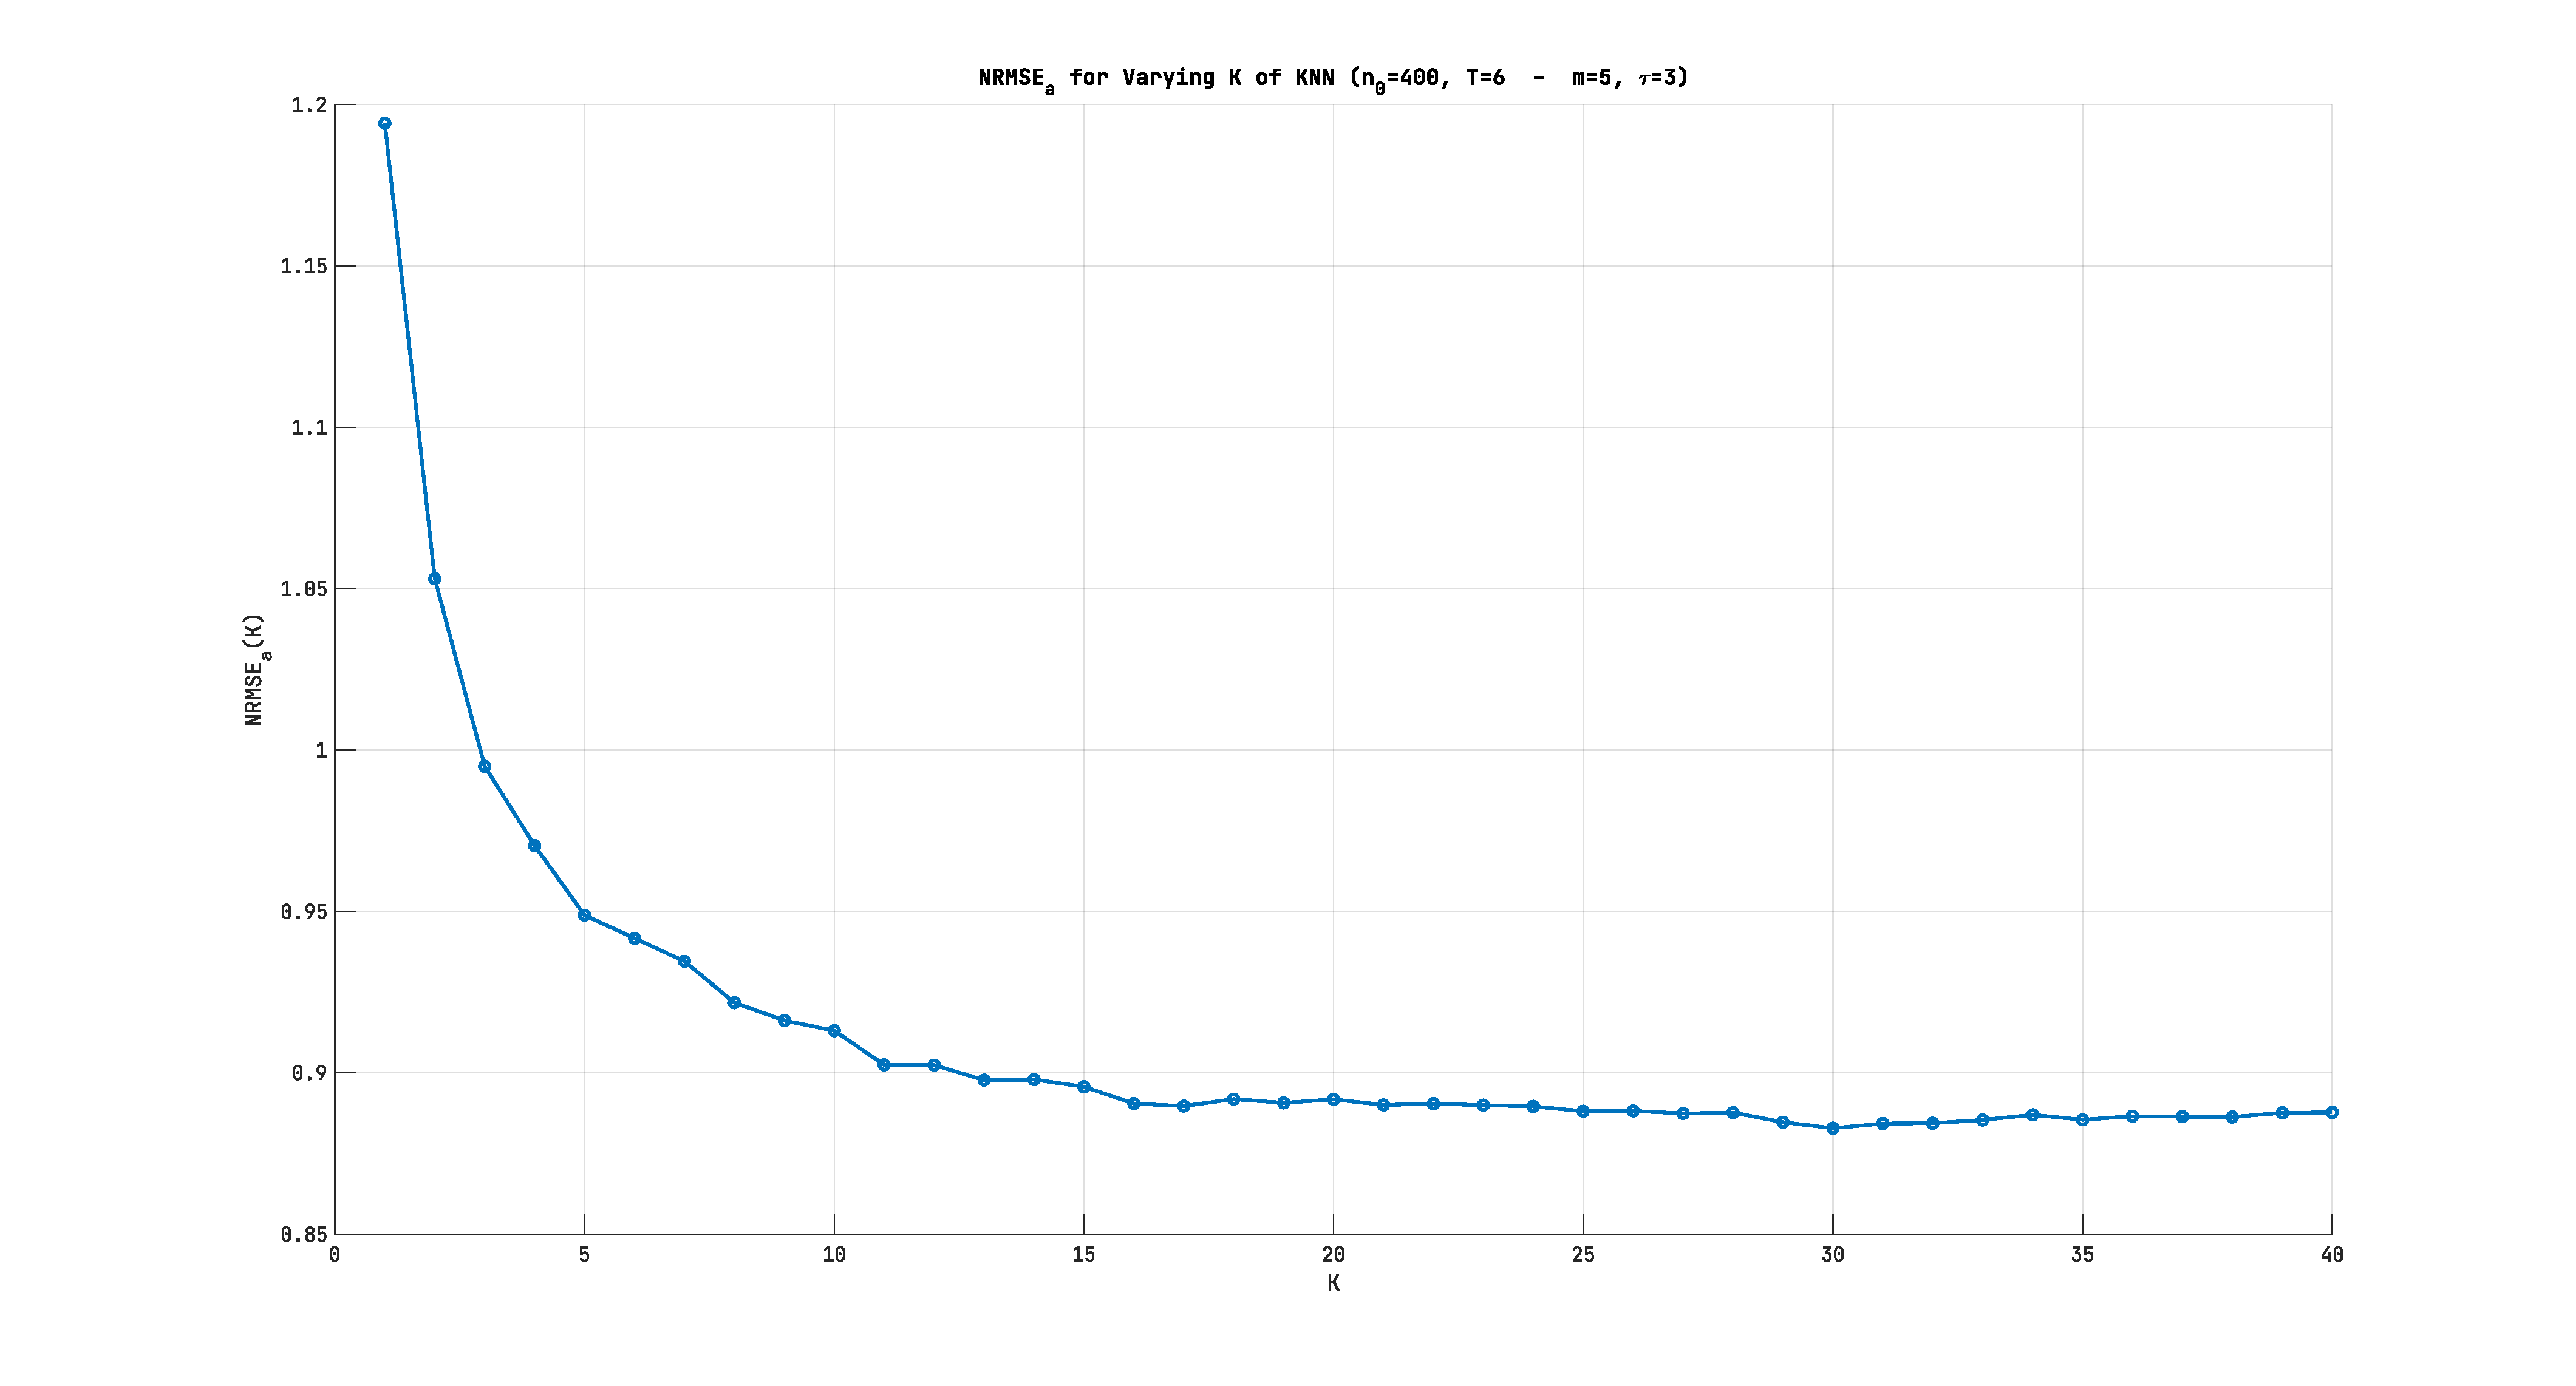
\includegraphics[width=\textwidth]{assets/images/plots/nrmse_k_a.svg.pdf}
        \caption{Διάγραμμα μεταβολής του μέσου \tl{NRMSE} των σφαλμάτων πρόβλεψης ως προς τον αριθμό των κοντινότερων γειτόνων που συμμετέχουν στη πρόβλεψη, $K$, για τη στάσιμη χρονοσειρά $\{X_a(t)\}$}
        \label{fig:nrmse_k_a}
    \end{center}
\end{figure}

Από το παραπάνω διάγραμμα επιλέγουμε για τιμή για τον αριθμό των κοντινότερων γειτόνων, $K \in [13, 16]$, με προτιμότερη τιμή το \textbf{\tl{K}=16}. Παρατηρούμε ότι για μικρές τιμές του $K$ η πρόβλεψη είναι χειρότερη από το να προβλέπαμε μόνιμα την μέση τιμή ($NRMSE>1$), ενώ καθώς ανεβαίνει ο αριθμός των γειτόνων που συμμετέχουν στη πρόβλεψη υπάρχει απότομη πτώση αρχικά, κατόπιν ένα \textquote{γόνατο} (στο οποίο προσπαθούμε να επιλέξουμε τις τιμές) και τέλος ένα πλατίασμα (\tl{plateau}) όπου περαιτέρω αύξηση οδηγεί σε μίκρες ή καθόλου αλλαγές του \tl{NRMSE}.

\subsection{Επιλογή του \tl{K} για τη στάσιμη χρονοσειρά \tl{B}}

Θα χρησιμοποιήσουμε και πάλι την δοθείσα συνάρτηση \texttt{\tl{localpredictmultistep}()} για να κάνουμε προβλέψεις και βρούμε τα σφάλματα πρόβλεψης για έως και $T$ βήματα εμπρός, με παραμέτρους:
\begin{itemize}
    \item \textit{Ορίζοντας Πρόβλεψης, Τ}: Θα χρησιμοποίσουμε την βέλτιστη τιμή που καταλήξαμε στο βήμα \ref{ch:step5}, δηλαδή $T=5$
    \item \textit{Διάσταση Εμβύθινσης, \tl{m}}: Θα χρησιμοποιήσουμε την τιμή που βρέθηκε από τη μέθοδο \tl{FNNs} εφαρμοζόμενη σε όλη τη στάσιμη χρονοσειρά Β, δηλαδή $m=5$
    \item \textit{Υστέρηση, τ}: Θα χρησιμοποιήσουμε την τιμή που βρέθηκε από τη συνάρτηση αμοιβαίας πληροφορίας ολόκληρης της στάσιμης χρονοσειράς Β, δηλαδή $\tau=2$
\end{itemize}

Παρακάτω εκτελούμε την συνάρτηση \texttt{\tl{localpredictmultistep}()}  για κάθε χρονική στιγμή με ορίσματα τις παραπάνω παραμέτρους καθώς και το $K=1,...,40$. Πλοτάρουμε το \tl{NRMSE} των σφαλμάτων πρόβλεψης και με βάση αυτό επιλέγουμε την καταλληλότερη τιμή για το $K$.

\begin{figure}[H]
    \begin{center}
        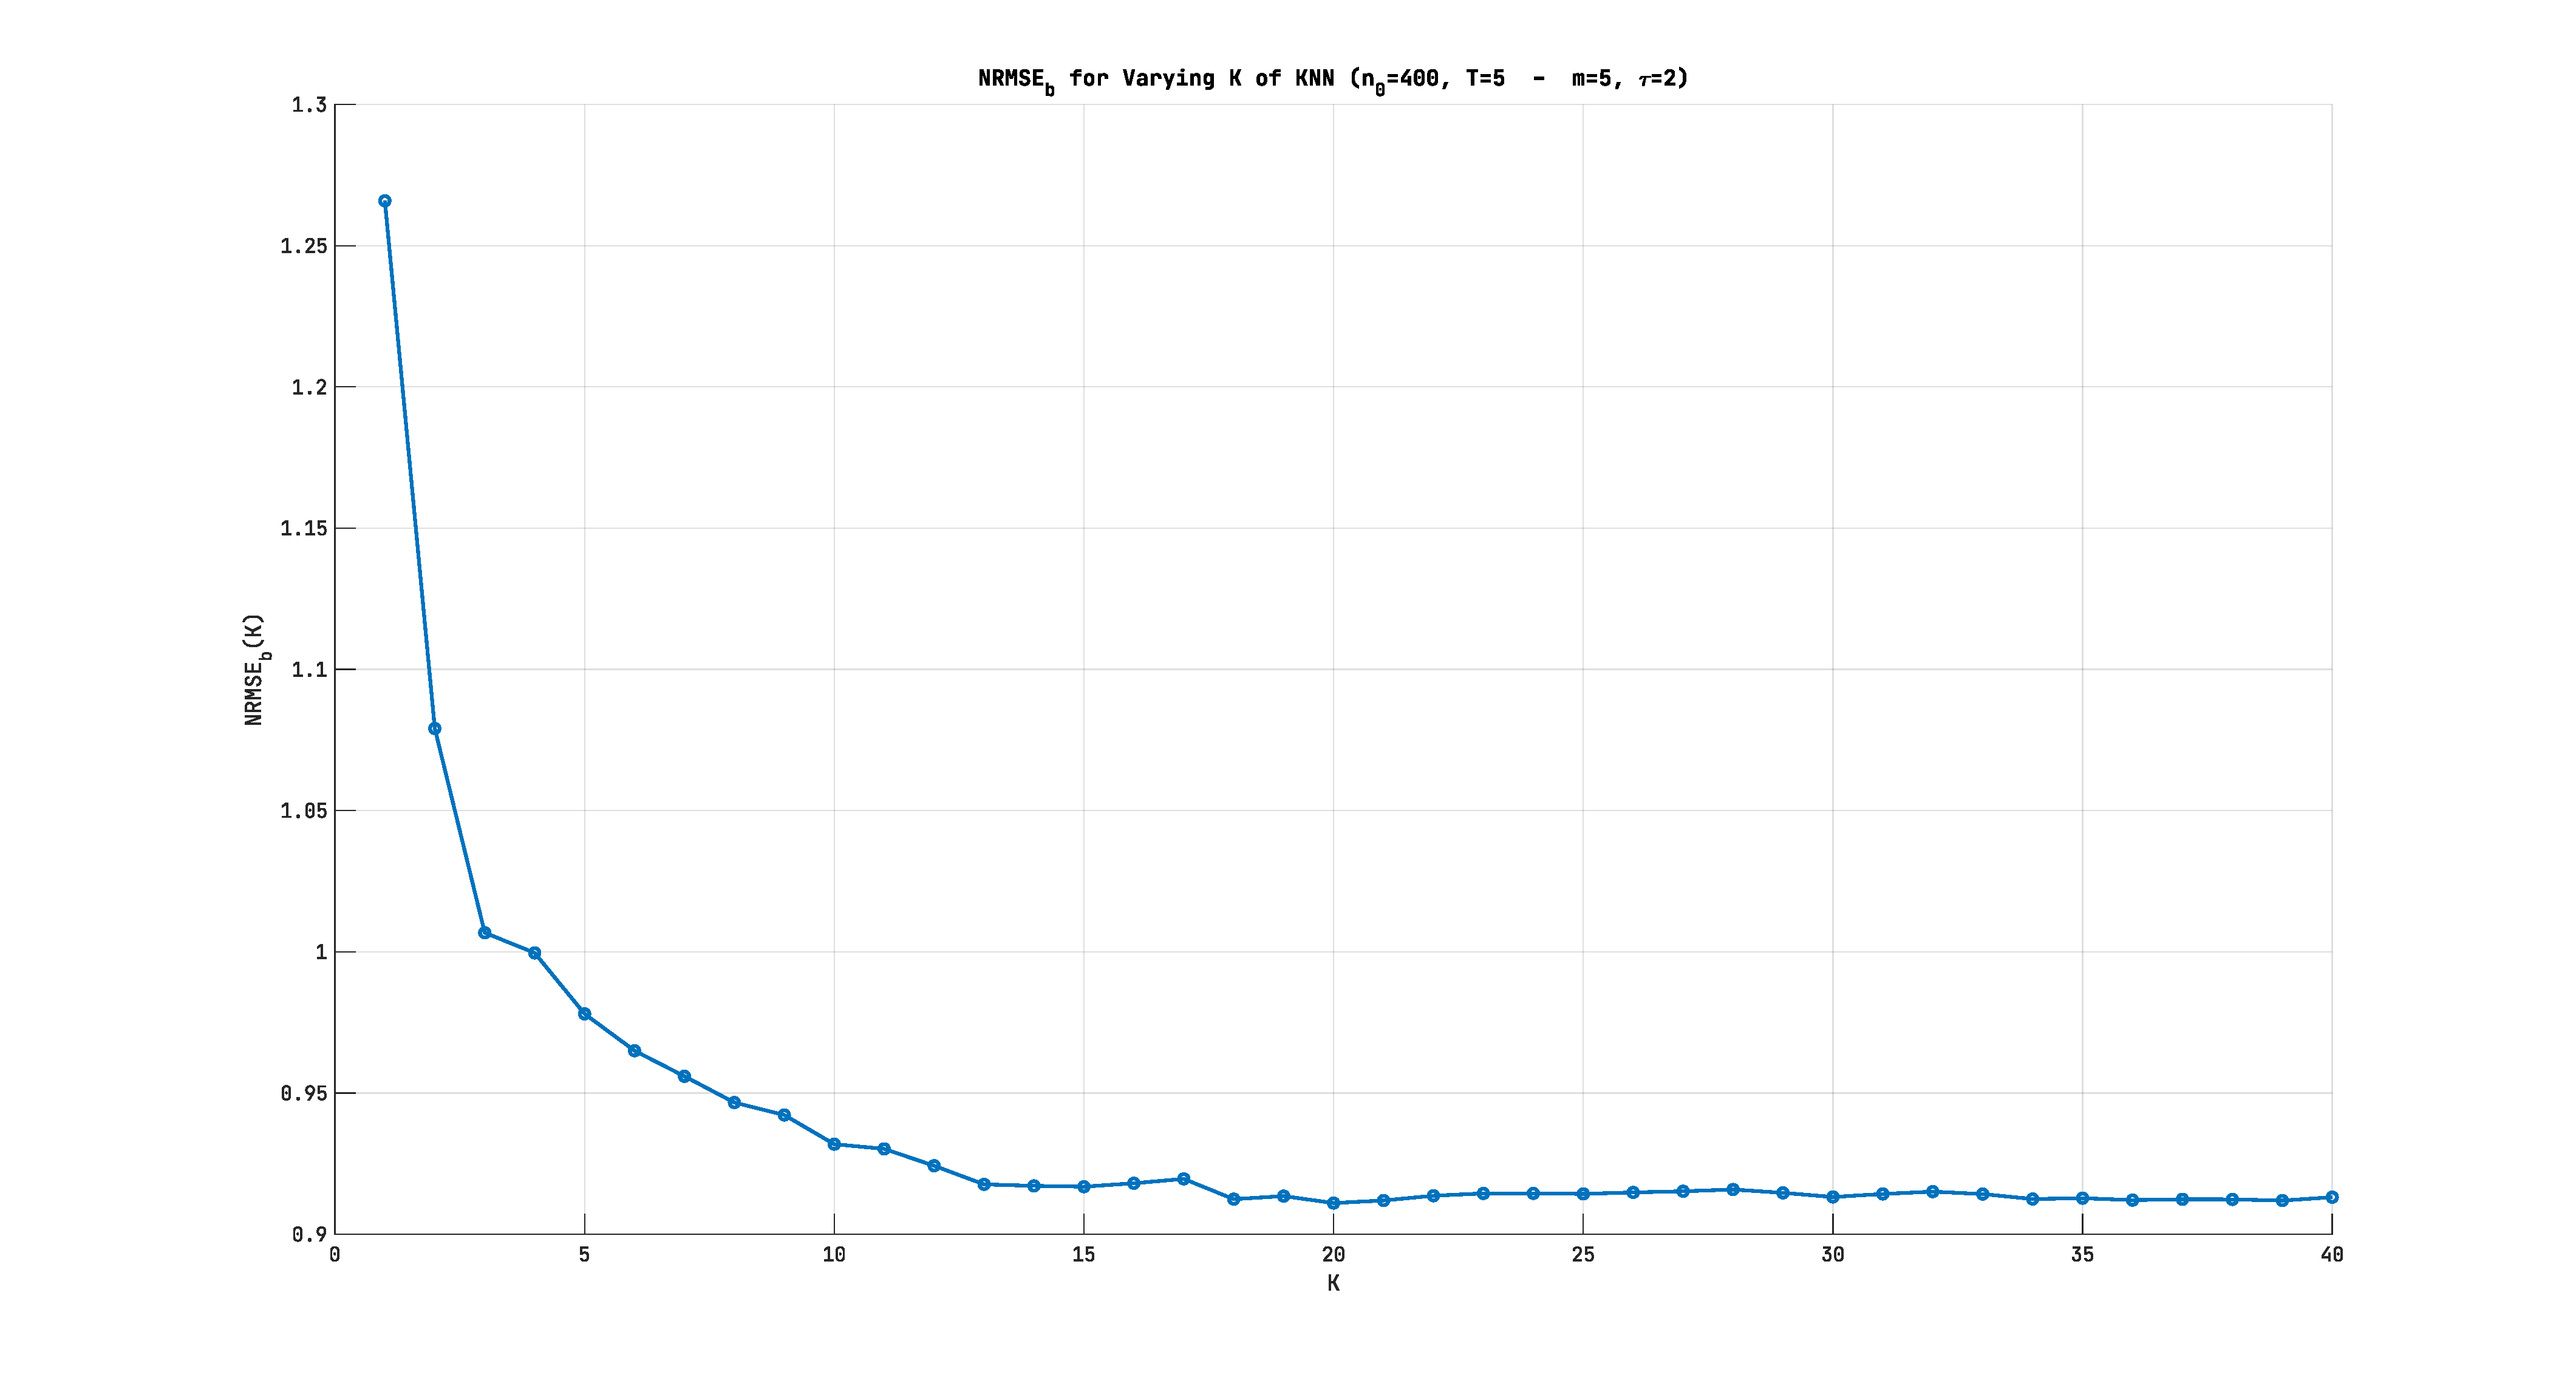
\includegraphics[width=\textwidth]{assets/images/plots/nrmse_k_b.svg.pdf}
        \caption{Διάγραμμα μεταβολής του μέσου \tl{NRMSE} των σφαλμάτων πρόβλεψης ως προς τον αριθμό των κοντινότερων γειτόνων που συμμετέχουν στη πρόβλεψη, $K$, για τη στάσιμη χρονοσειρά $\{X_{b_{deseasoned}}(t)\}$}
        \label{fig:nrmse_k_b}
    \end{center}
\end{figure}

Από το παραπάνω διάγραμμα επιλέγουμε για τιμή για τον αριθμό των κοντινότερων γειτόνων, \textbf{\tl{K}=13}. Το διάγραμμα αυτό έχει παρόμοια μορφή με το αντίστοιχο για τη στάσιμη χρονοσειρά Α (σχήμα \ref{fig:nrmse_k_a}) όποτε ισχύουν και εδώ τα αντίστοιχα σχόλια.


\section{Εφαρμογή Τοπικού Μοντέλου Κοντινότερων Γειτόνων για Εξαγωγή Σημείων Αλλαγής}

Για την εύρεση των σημείων αλλαγής θα χρησιμοποιηθεί η ίδια μέθοδος που χρησιμοποιήθηκε για τα γραμμικά μοντέλα, σχέση (\ref{eq:s_n}), επίσης \textbf{εφαρμοζόμενη στις στάσιμες χρονοσειρές}, $\{X_a(t)\}$ και $\{X_{b_{deseasoned}}(t)\}$ αντίστοιχα. Ωστόσο αντί κάθε φόρα να προσαρμόζεται ένα γραμμικό μοντέλο τύπου $ARMA$ και να γίνονται οι προβλέψεις βάσει αυτού, εδώ θα προσαρμόζεται ένα μη-γραμμικό, τοπικό μοντέλο κοντινότερων γειτόνων, και οι προβλέψεις θα γίνονται βάσει της σχέσης (\ref{eq:x_i_1_knn}).

Θα εργαστούμε ξεχωριστά σε κάθε μία από τις στάσιμες χρονοσειες Α και Β. Για κάθε μία, θα παρουσιάσουμε τα \tl{surf plots} από τα οποία θα δούμε έαν μπορούμε να εφαρμόσουμε την μέθοδο με τις παραμέτρους ($T$ και $\lambda_{std}$) που επιλέχθηκαν για τα γραμμικά μοντέλα, ή, εάν όχι, ποιες τίμες θα επιλέγαμε για τα μη-γραμμικά μοντέλα. Στη συνέχεια θα τρέξουμε τη μέθοδο για κάθε μία χρησιμοποιώντας τις αντίστοιχες βέλτιστες παραμέτρους, ενώ στο τέλος θα δωθούν τα διάγραμματα τόσο των στάσιμων όσο και των αρχικών χρονοσειρών με τοποθετημένα τα σημεία αλλαγής που εξήχθησαν.

\par Όπως και για τα γραμμικά, έτσι και εδώ κατά τη διάρκεια του \tl{grid search} το μοντέλο \textbf{αναπροσαρμόζεται με βάση την επιλογή \textquote{\tl{c}}}, δηλαδή παραμένει σταθερό έως ότου βρεθεί σημείο αλλαγής και προσαρμόζεται στις 400 τελευταίες παρατηρήσεις από το σημείο αλλαγής + T. 
\\ \\\textit{Η αναπροσαρμογή εδώ σημαίνει απλώς \textbf{επαναϋπολογισμός του $\alpha=\lambda_{std}*s_x$}, καθώς το μη γραμμικό μοντέλο υπολογίζει και κάνει προβλέψεις ταυτόχρονα, άρα σε κάθε χρονική στιγμή.}

\subsection{Εφαρμογή στη στάσιμη χρονοσειρά Α}

Για να τρέξει το \tl{grid search} θέτουμε τη τιμή \textbf{\tl{K}=16 κοντινότερους γείτονες} σύμφωνα με τη τιμή που προέκυψε από το σχήμα \ref{fig:nrmse_k_a}.

\subsubsection{Επιλογή Βέλτιστων Παραμέτρων}

Για επιλογή βέλτιστων τιμών στις \tl{hyperparameters} της μεθόδου και συγκεκριμένα στον ορίζοντα πρόβλεψης, $T$, και στο $\lambda_{std}$ του ορίου απόφασης, $\alpha$, θα κάνουμε αναζήτηση πλέγματος ως προς αυτές. Ως μετρικές για αξιολόγηση του κάθε συνδυασμού των παραμέτρων αυτών χρησιμοποιήθηκαν και εδώ ο \textit{Αριθμός των σημειών αλλαγής \tl{MCPs}} (Θέλουμε να μην είναι πολύ μεγάλος καθώς κάτι τέτοιο κάνει λιγότερο αξιόπιστη την όλη μέθοδο, αλλά να μην είναι και πολύ μικρός ώστε να υπάρχει νόημα χρήσης της μεθόδου), και το \textit{\tl{NRMSE} των προβλέψεων} (θέλουμε κατά το δυνατό μικρότερο).

Αρχικά παραθέτονται σε διαγράμματα τύπου \tl{surf} τα αποτελέσματα αναζήτησης πλέγματος ως προς τις παραπάνω μετρικές για τη στάσιμη χρονοσειρά $\{X_a(t)\}$, ενώ στη συνέχεια σχολιάζεται ο τρόπος επιλογής προσεγγεστικά βέλτιστων παραμάτρων αλλά και οι τελικές τους τιμές.

\begin{figure}[H]
    \begin{center}
        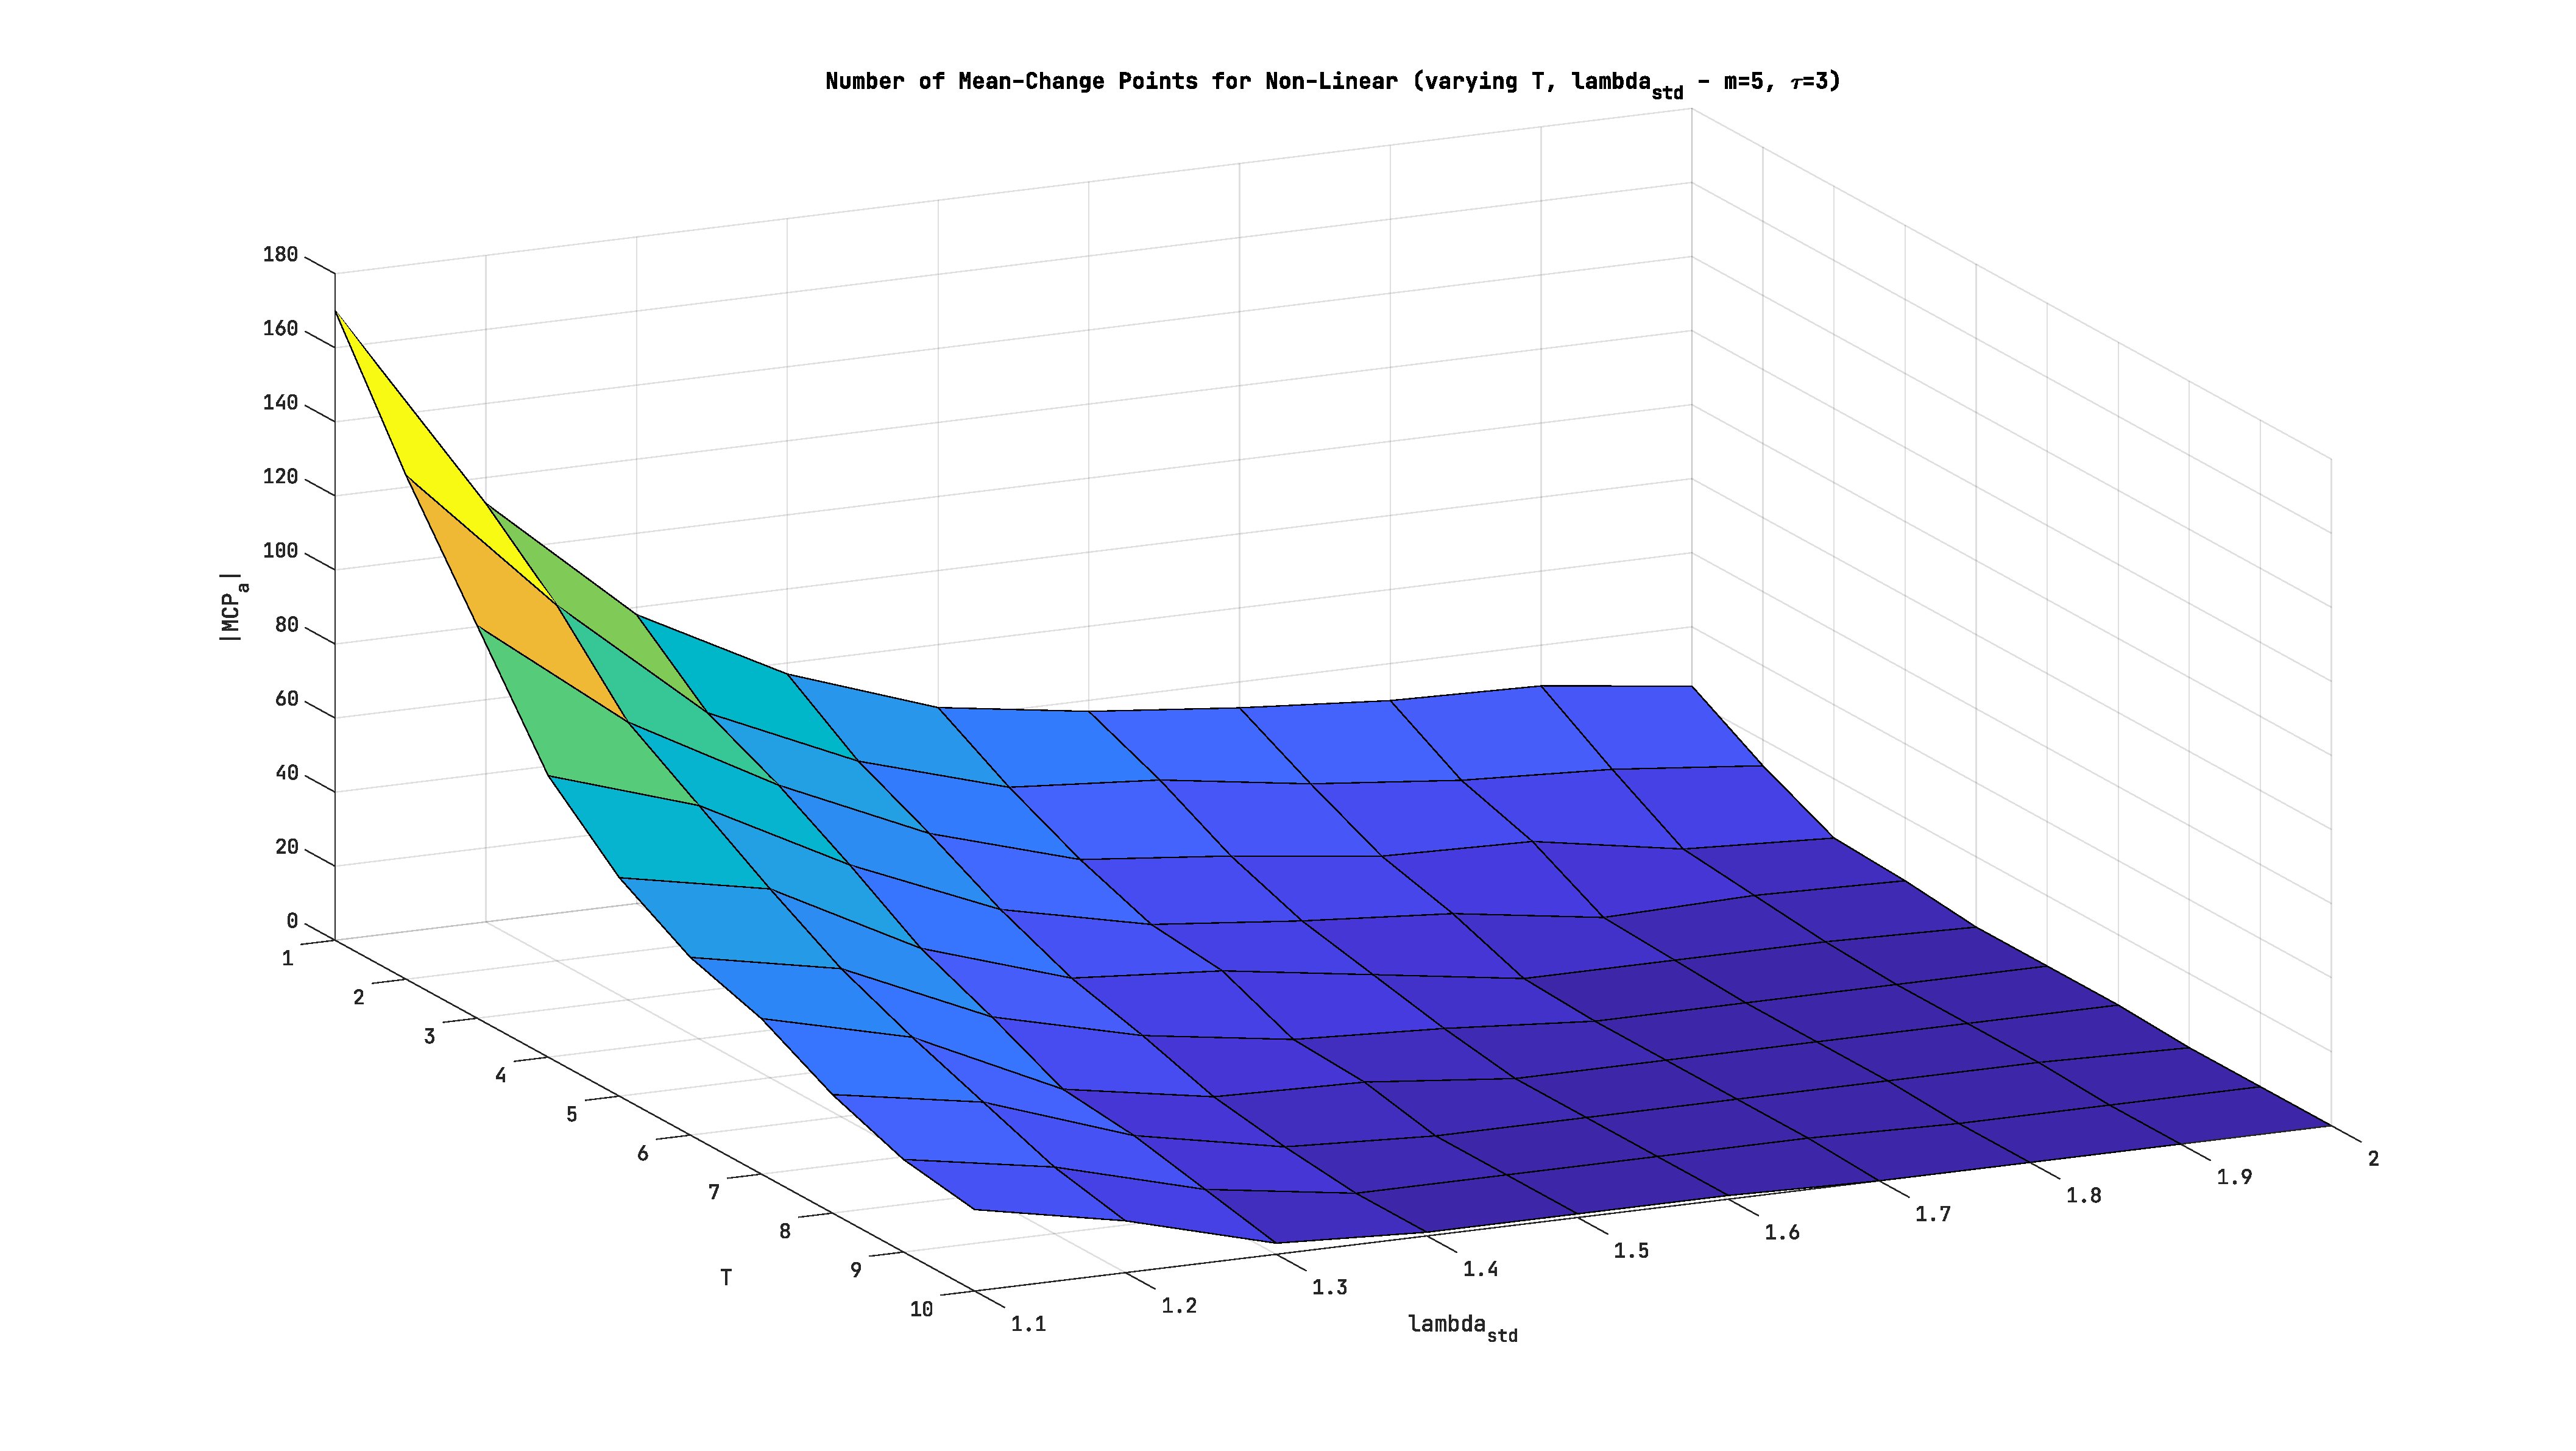
\includegraphics[width=\textwidth]{assets/images/plots/mcps_count_nl_a.svg.pdf}
        \caption{Αριθμός σημείων αλλαγής της στάσιμης χροσνοσειράς Α, $\vert$\tl{MCP}$\vert$, που προκύπτουν για κάθε τιμή του πλέγματος αναζήτησης ως πρός τον ορίζοντα πρόβλεψης, $T$, και το $\lambda_{std}$ του ορίου απόφασης, $\alpha$, για παραμέτρους μη-γραμμικού μοντέλου $m=5$, $\tau=3$ και $K=16$}
        \label{fig:mcps_count_nl_a}
    \end{center}
\end{figure}

\begin{figure}[H]
    \begin{center}
        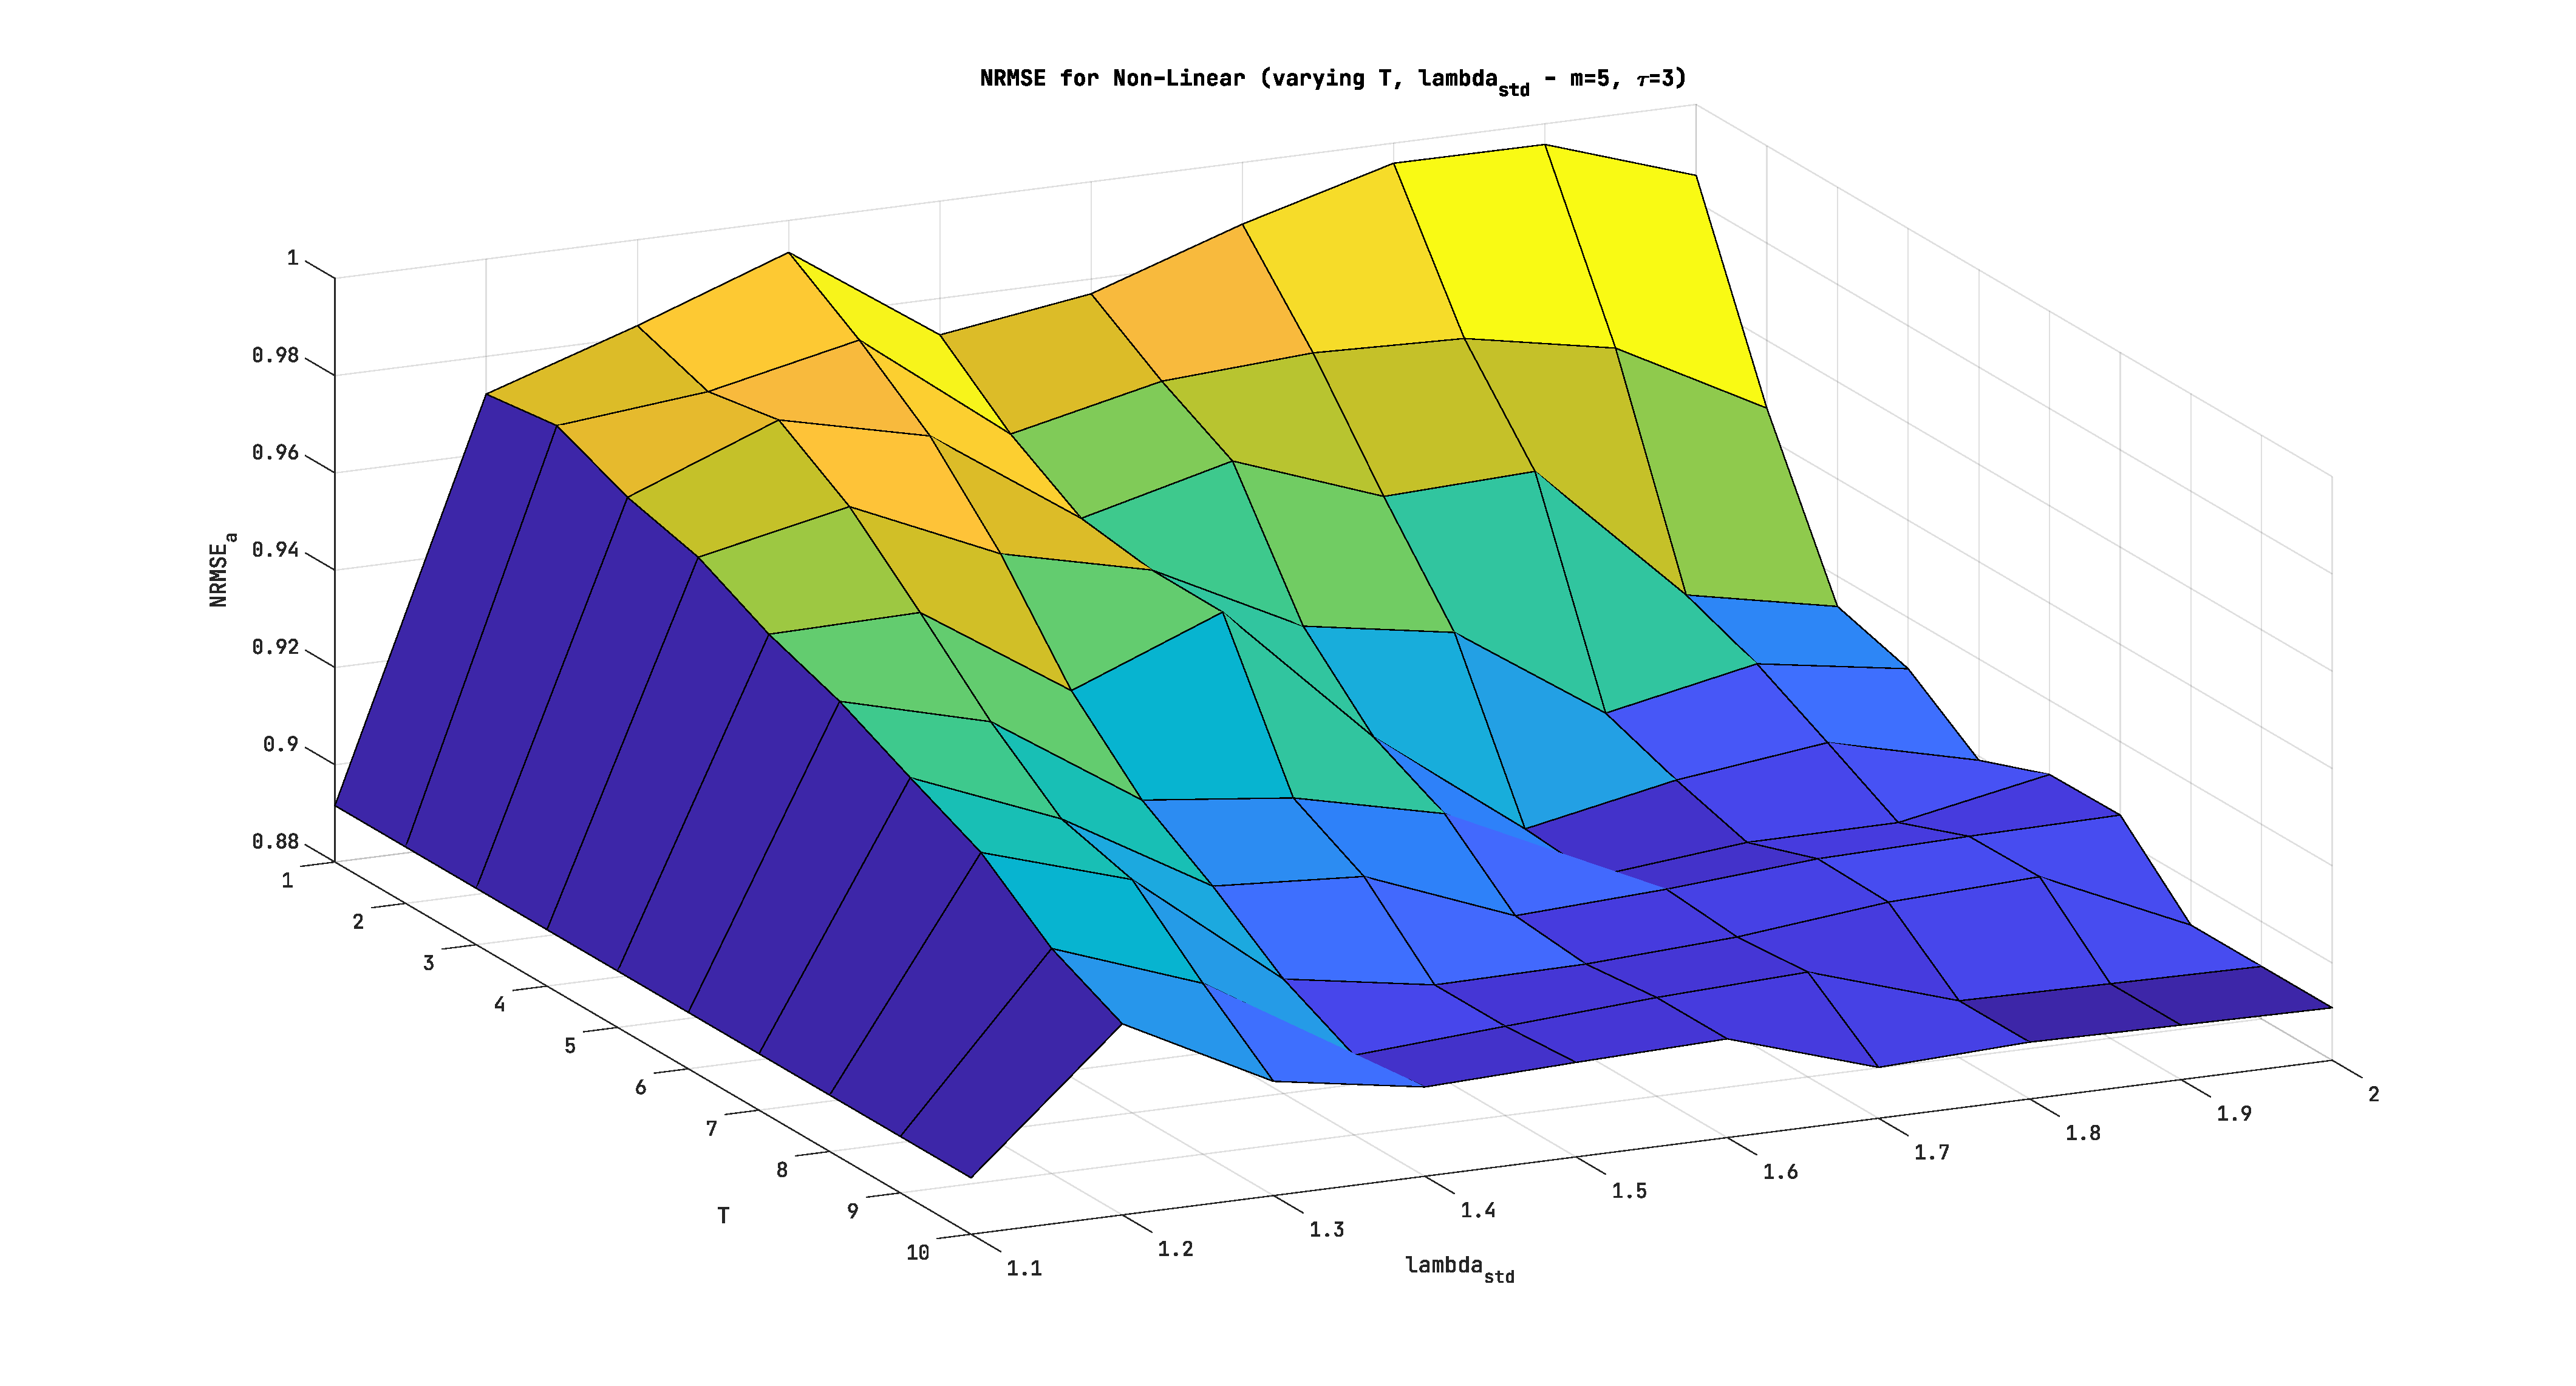
\includegraphics[width=\textwidth]{plots/nrmse_nl_a.svg.pdf}
        \caption{\tl{NRMSE} προβλέψεων κατά τον υπολογισμό των σημείων αλλαγής (\tl{MCPs}) της στάσιμης χροσνοσειράς Α, για κάθε τιμή του πλέγματος αναζήτησης ως πρός τον ορίζοντα πρόβλεψης, $T$, και το $\lambda_{std}$ του ορίου απόφασης, $\alpha$, για παραμέτρους μη-γραμμικού μοντέλου $m=5$, $\tau=3$ και $K=16$}
        \label{fig:nrmse_nl_a}
    \end{center}
\end{figure}

\par Γενικότερα, αναζητούμε τα \textquote{γόνατα} στις αντίστοιχες τρισδιάστατες καμπύλες έτσι ώστε περαιτέρω μεταβολές των αντίστοιχων παραμέτρων να μην είναι πλέον επικερδείς.

\par Επικεντρώνοντας στο πρώτο διάγραμμα και δεδομένου ότι θέλουμε ο αριθμός των \tl{MCPs} να μήν είναι πολύ μεγάλος ή πολύ μικρός, θα επιλέγαμε τις ακόλουθες τιμές (προσεγγιστικά):
\begin{align}
    T \in [6,10] \ \ \ \& \ \ \ \lambda_{std} \in [1.2, 1.5]
    \label{eq:t_lambda_mcps_nl_a}
\end{align}

\par Επικεντρώνοντας τώρα στο διάγραμμα των \tl{NRMSEs} και δεδομένου ότι θέλουμε το \tl{NRMSE} να είναι κατά το δυνατό μικρό, θα επιλέγαμε τις ακόλουθες τιμές (προσεγγιστικά):
\begin{align}
    T \geq 5 \ \ \ \& \ \ \ \lambda_{std} \geq 1.3
    \label{eq:t_lambda_nrmses_nl_a}
\end{align}

\par Συνδυάζοντας τις σχέσεις (\ref{eq:t_lambda_mcps_nl_a}) και (\ref{eq:t_lambda_nrmses_nl_a}) παραπάνω καταλήγουμε ότι οι \tl{hyperparameters} που θα χρησιμοποιηθούν για την εφαρμογή της μεθόδου αυτόματης εύρεσης χρονικών σημείων αλλαγής θα είναι:
\textbf{T = 6 βήματα} και \textbf{λ\textsubscript{\tl{std}} = 1.5}. Οι αντίστοιχες τιμές του \tl{grid search} είναι: \textbf{$\vert$\tl{MCP}$\vert$ = 8 \tl{MCPs}} και \textbf{\tl{NRMSE} = 0.92}.

\par Η τελική επιλογή παραπάνω έγινε με βάση το μικρότερο \tl{NRMSE}. Τυχγάνει λοιπόν στη στάσιμη χρονοσειρά Α, οι παράμετροι της μεθόδου να ίδιες για τα γραμμικά και μη-γραμμικά μοντέλα.

\par Τέλος, φαίνεται πως η χρήση του μη-γραμμικού, τοπικού μοντέλου $K=16$\ \ κοντινότερων γειτόνων εμφανίζει μεγαλύτερο \tl{NRMSE} κατά την εφαρμογή της μεθόδου εξαγωγής σημείων αλλαγής σε σύγκριση με τη χρήση γραμμικού μοντέλου $MA(1)$.

\subsubsection{Εφαρμογή Μεθόδου με Βέλτιστες Παράμετρους}

Χρησιμοποιώντας τις επιλεγμένες τιμές για τις \tl{hyperparameters} της μεθόδου, δηλαδή ορίζοντα πρόβλεψης έως και 6 βημάτων εμπρός, $T=6$, παράμετρο ορίου απόφασης στο 1.5, $\lambda_{std}=1.5$, διάσταση εμβύθινσης, $m=5$, υστέρηση, $\tau=3$ και αριθμό κοντινότερων γειτόνων, $K=16$, θα τρέξουμε την παραπάνω μέθοδο στη στάσιμη χρονοσειρά που προέκυψε από το βήμα \ref{ch:step1}, $\{X_a(t)\}$, κάνοντας προβλέψεις με το μη-γραμμικό τοπικό μοντέλο μέσου όρου. Παρακάτω, φαίνονται τα σημεία αλλαγής που προκύπτουν από την εκτέλεση της μεθόδου με τις παραπάνω παραμέτρους για κάθε μια από τις επιλογές αναπροσαρμογής του μοντέλου (\textquote{\tl{a}}, \textquote{\tl{b}} ή \textquote{\tl{c}}).

\paragraph{Αναπροσαρμογή όταν βρεθεί σημείο αλλαγής}- Επιλογή \textquote{\tl{c}}

\begin{figure}[H]
    \begin{center}
        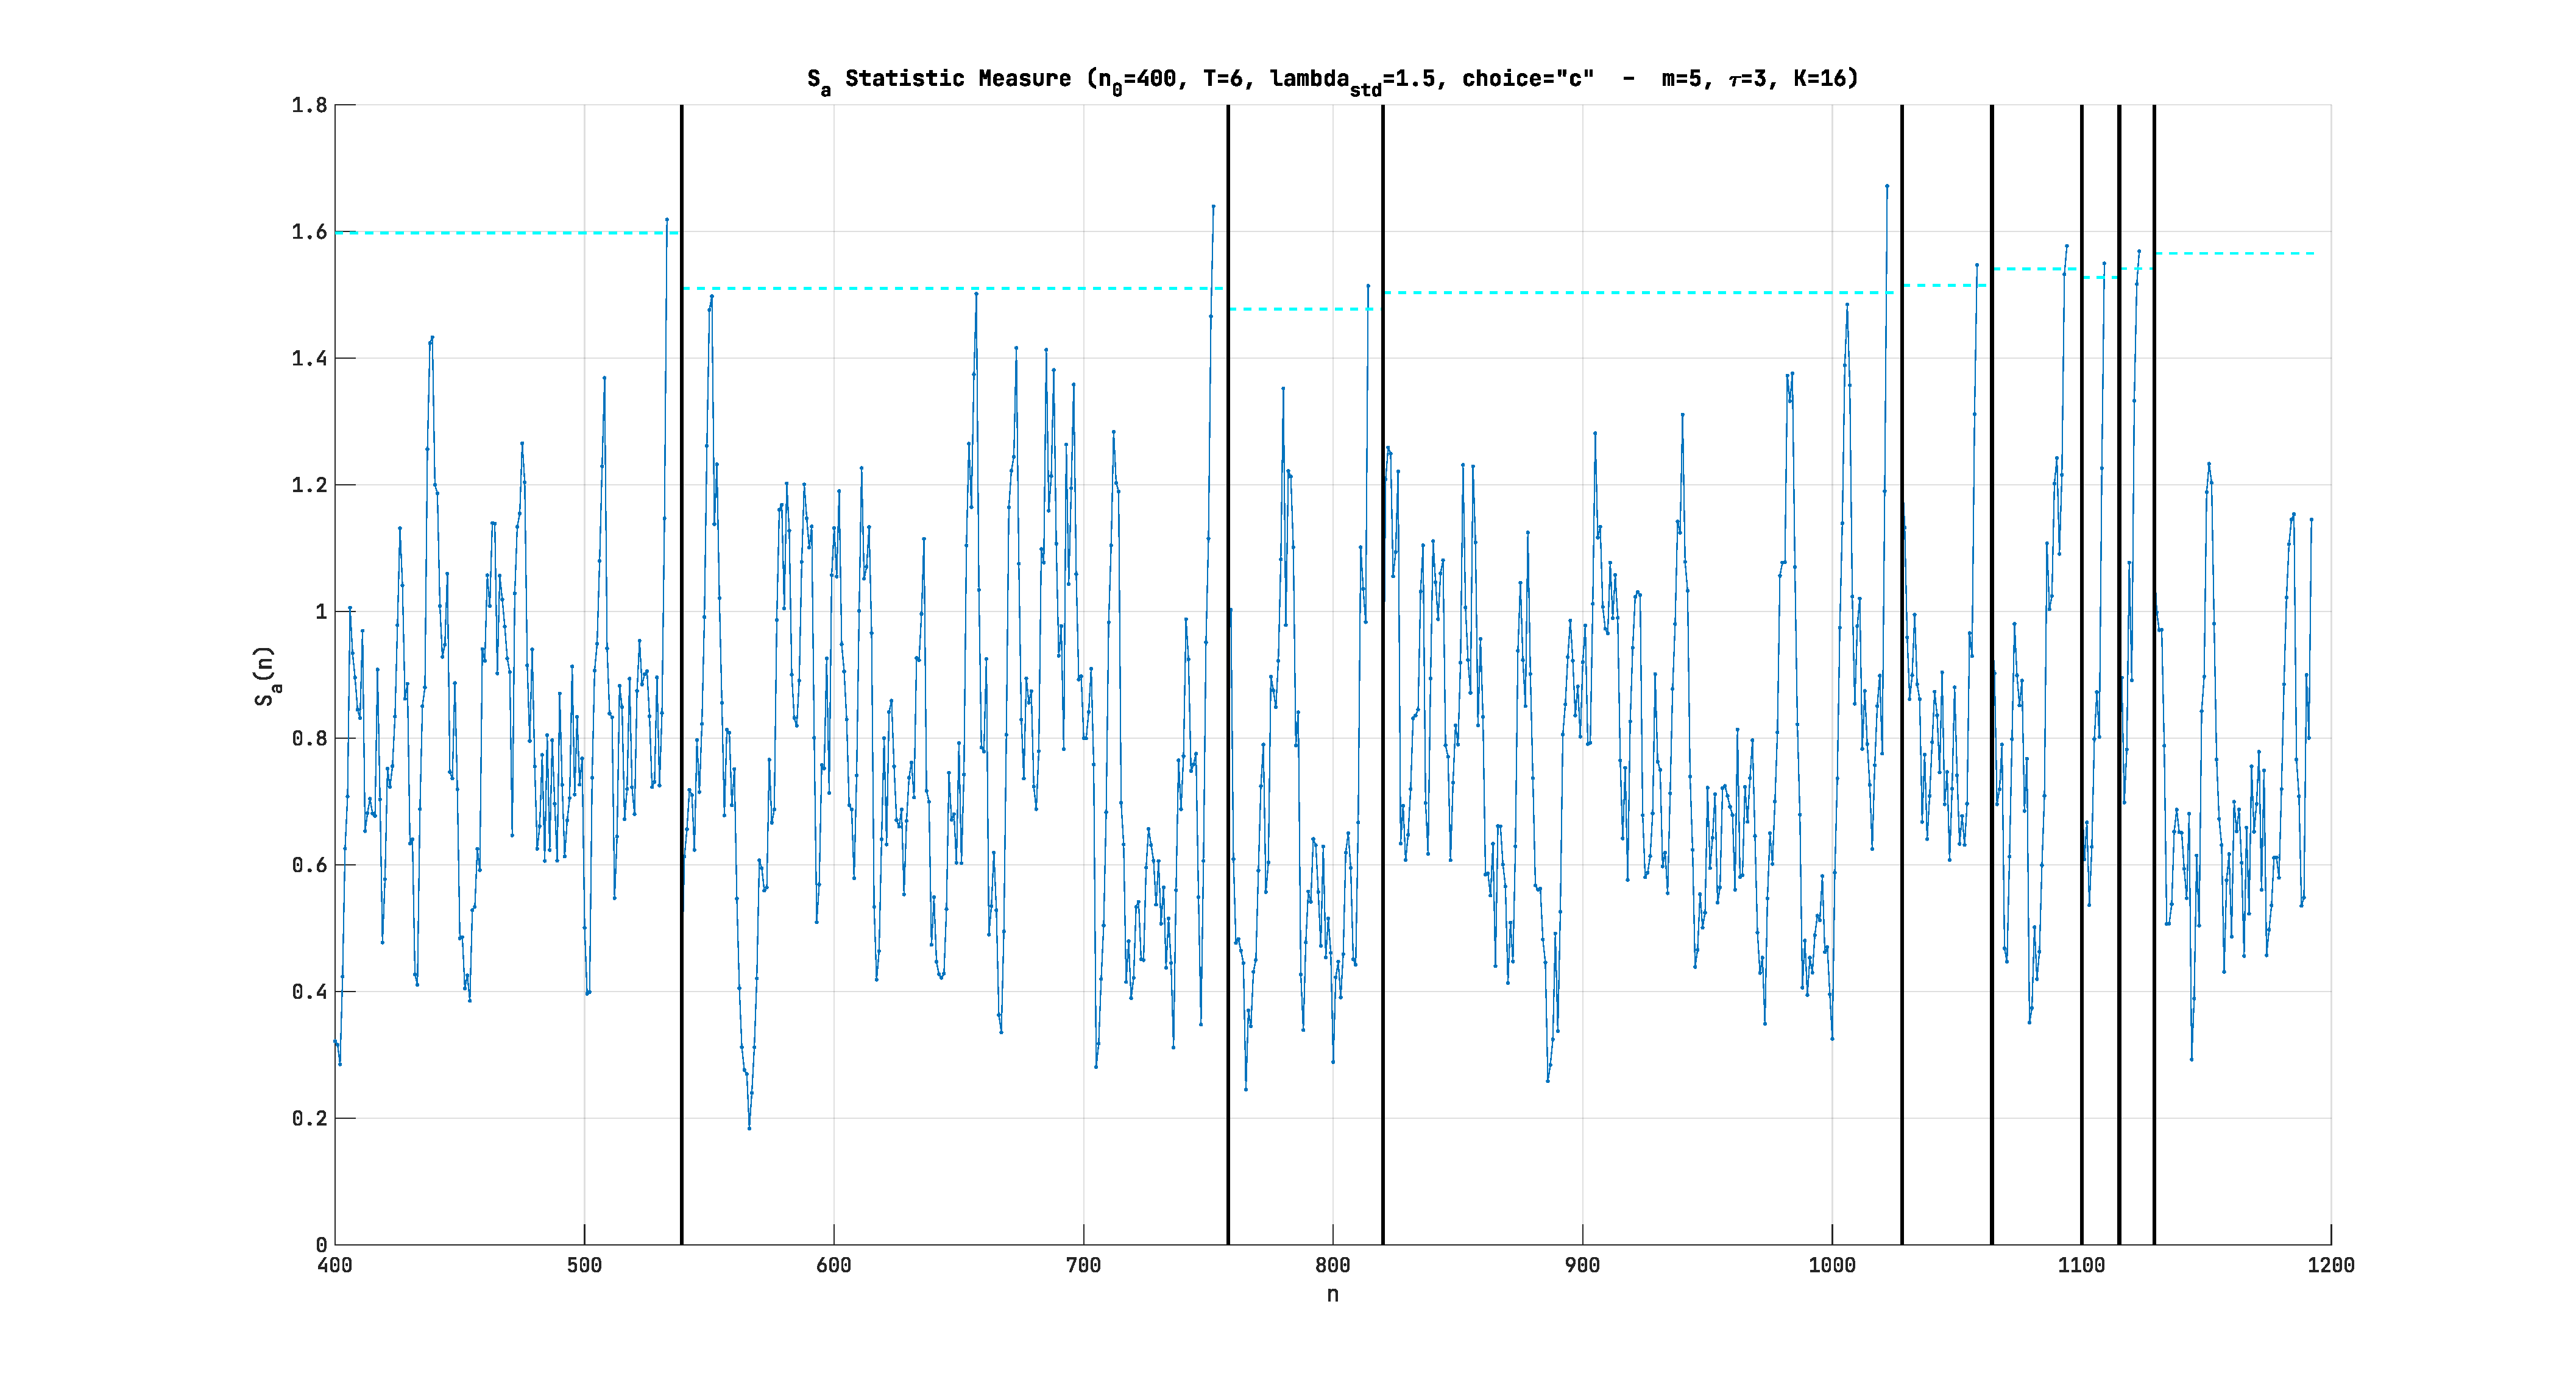
\includegraphics[width=\textwidth]{plots/mcps_nl_xa_opt_c.svg.pdf}
        \caption{Τιμές στατιστικού $S_n$ για έως και 6 βήματα μπροστά πρόβλεψη με τοπική πρόβλεψη μέσου Κ=16 κοντινότερων γειτόνων της στάσιμης χρονοσειράς $\{X_a(t)\}$ και για επιλογή αναπροσαρμογής \textquote{\tl{c}} (αναπροσαρμογή όταν βρεθεί σημείο αλλαγής). Σημειώνονται επίσης το κριτήριο απόφασης, $\alpha=1.5*s_x$, (\tl{cyan}) και φυσικά τα σημεία αλλαγής με έντονες κάθετες γραμμές στα εκάστοτε σημεία $n+T$ (μαύρο) - [\tl{NRMSE}=0.92, \ 0.6\tl{sec}]}
        \label{fig:mcps_nl_xa_opt_c}
    \end{center}
\end{figure}

Παρακάτω, τα ίδια σημεία αλλαγής απεικονίζονται στην αρχική χρονοσειρά προβολών του βίντεο \tl{A}:

\begin{figure}[H]
    \begin{center}
        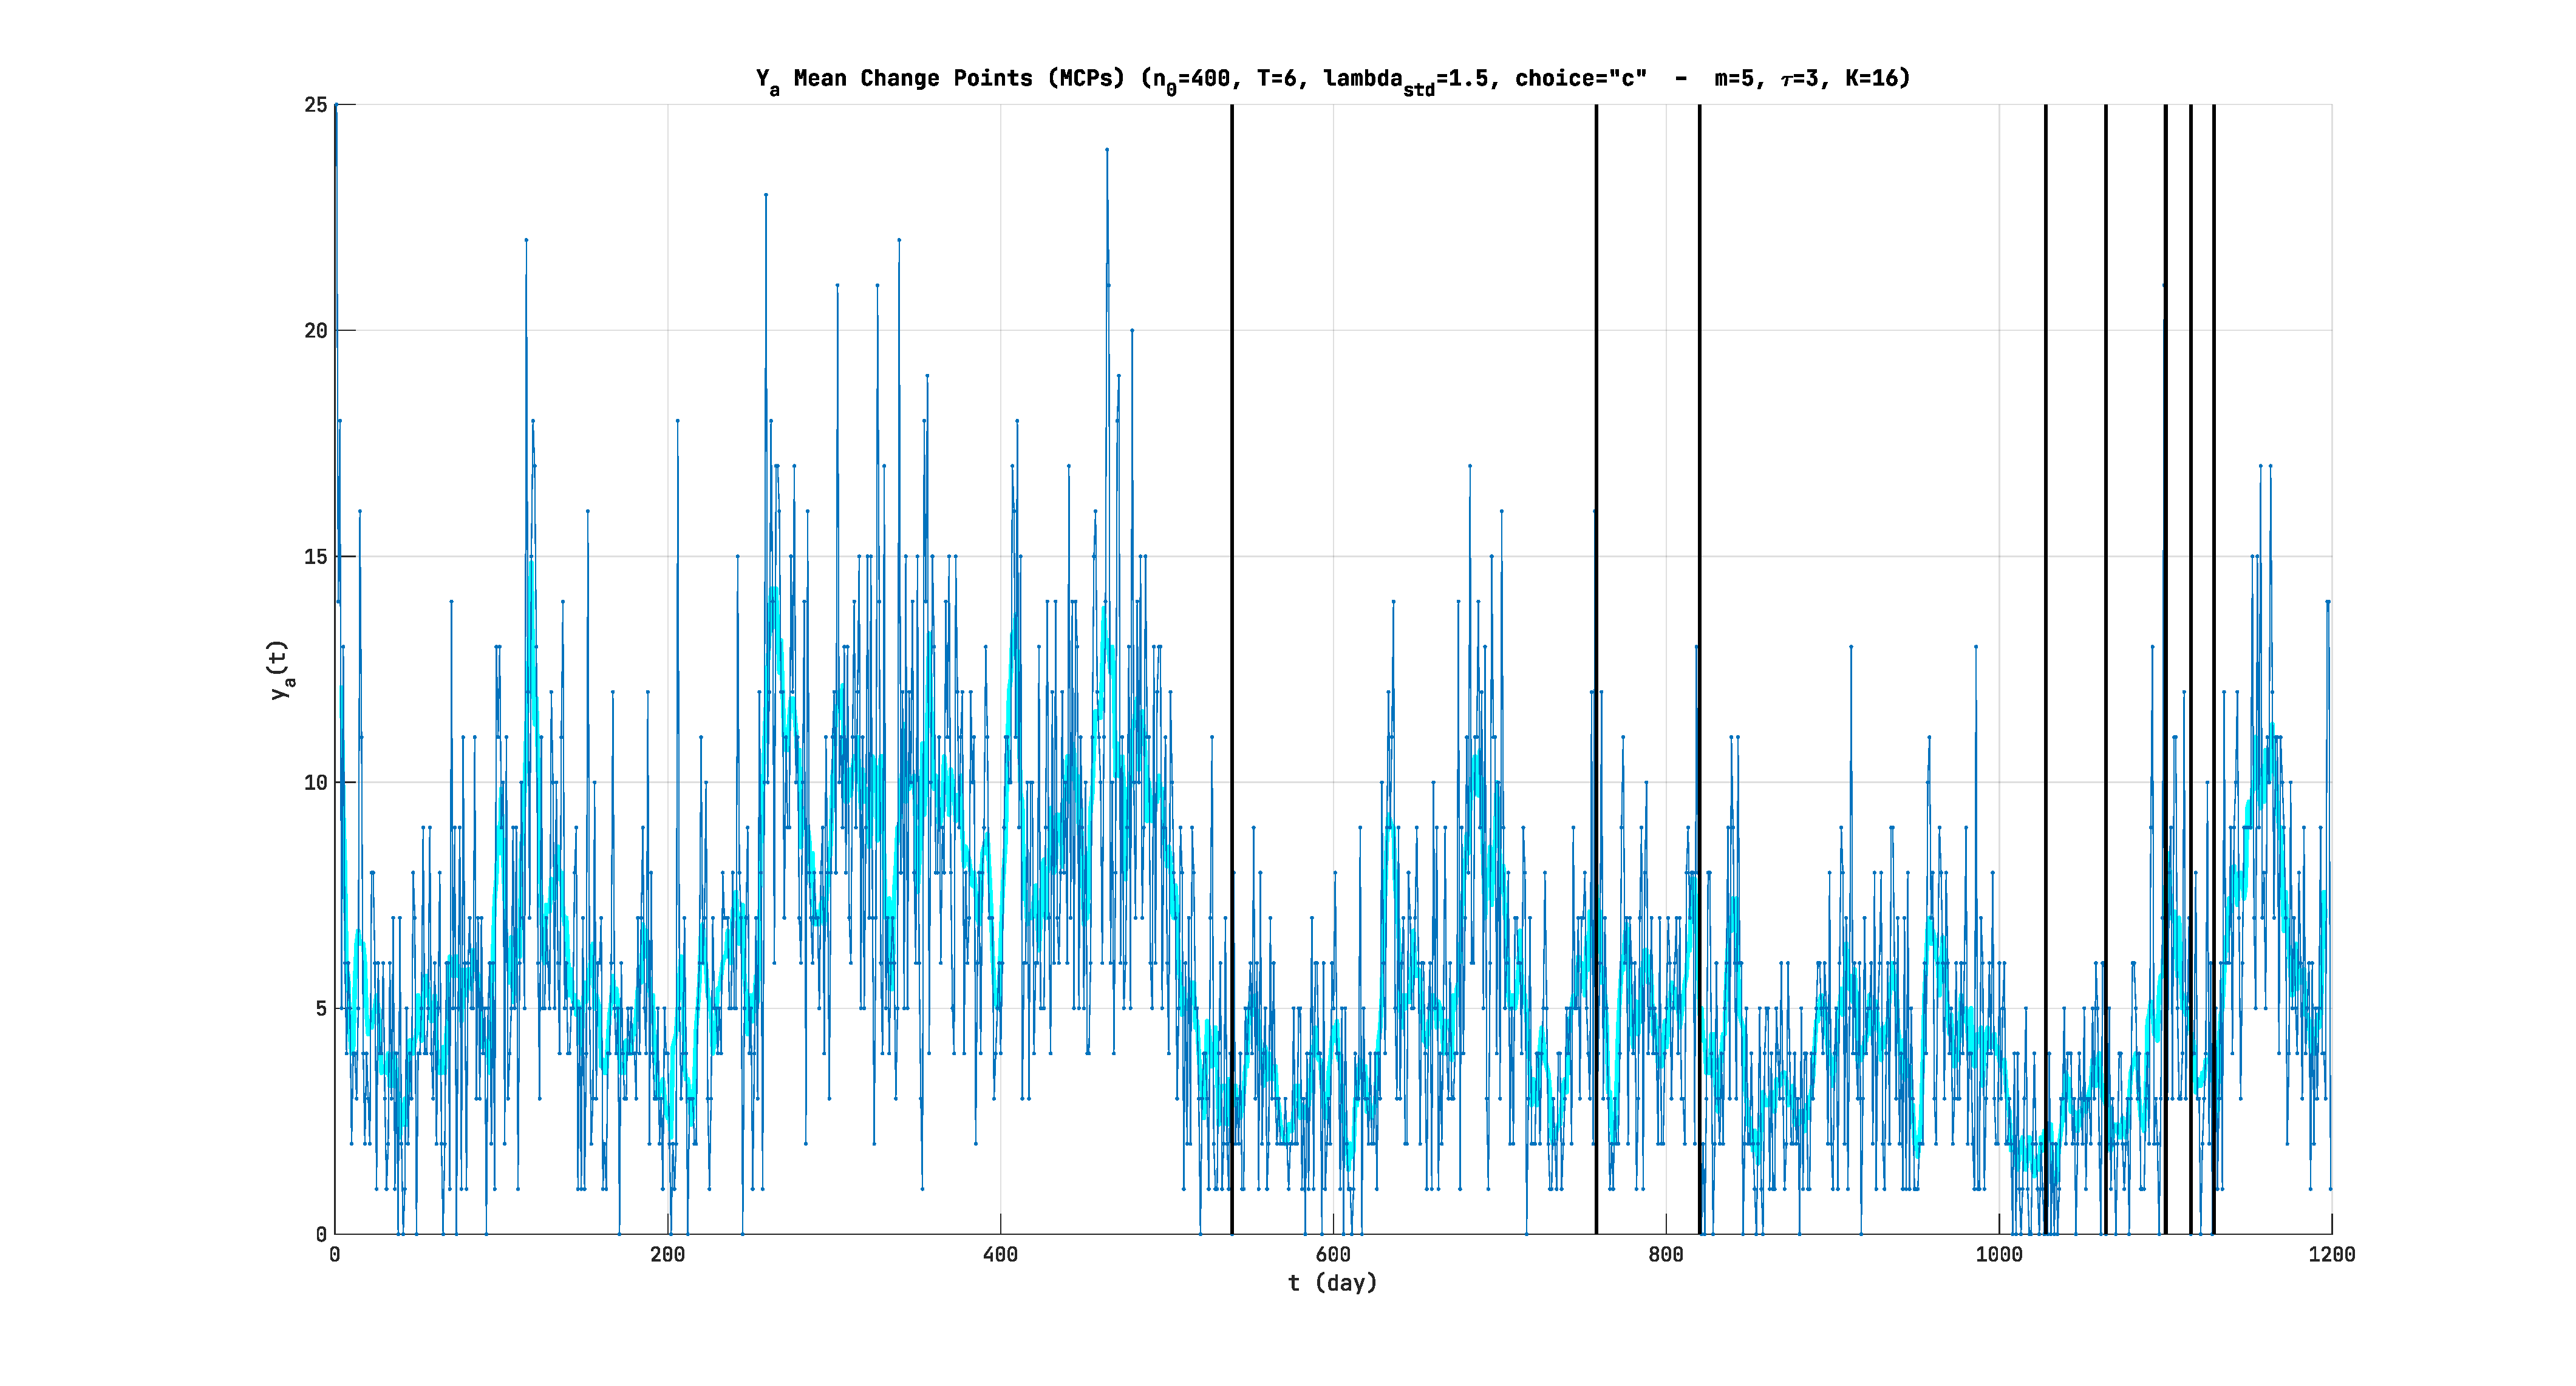
\includegraphics[width=\textwidth]{plots/mcps_nl_ya_opt_c.svg.pdf}
        \caption{Διάγραμμα ιστορίας της αρχικής χρονοσειράς $\{Y_a(t)\}$ (μπλε) μαζί με τα σημεία αλλαγής (μαύρο) που επιλέχθηκαν από τη μη-γραμμική ανάλυση της στάσιμης εκδοχής της με τις βέλτιστες παραμέτρους, καθώς και εκτίμηση της τάσης με φίλτρο κινούμενου μέσου τάξης 7 ($MA(7)$ \tl{smoothing}) - επιλογή \textquote{\tl{c}}}
        \label{fig:mcps_nl_ya_opt_c}
    \end{center}
\end{figure}

\paragraph{Αναπροσαρμογή σε κάθε χρονική στιγμή}- Επιλογή \textquote{\tl{b}}

Τα ίδια διαγράμματα παρουσιάζονται για την επιλογή αναπροσαρμογής \textquote{\tl{b}} (αναπροσαρμογή σε κάθε χρονική στιγμή) ενώ ακολουθεί σύντομος σχολιασμός:

\begin{figure}[H]
    \begin{center}
        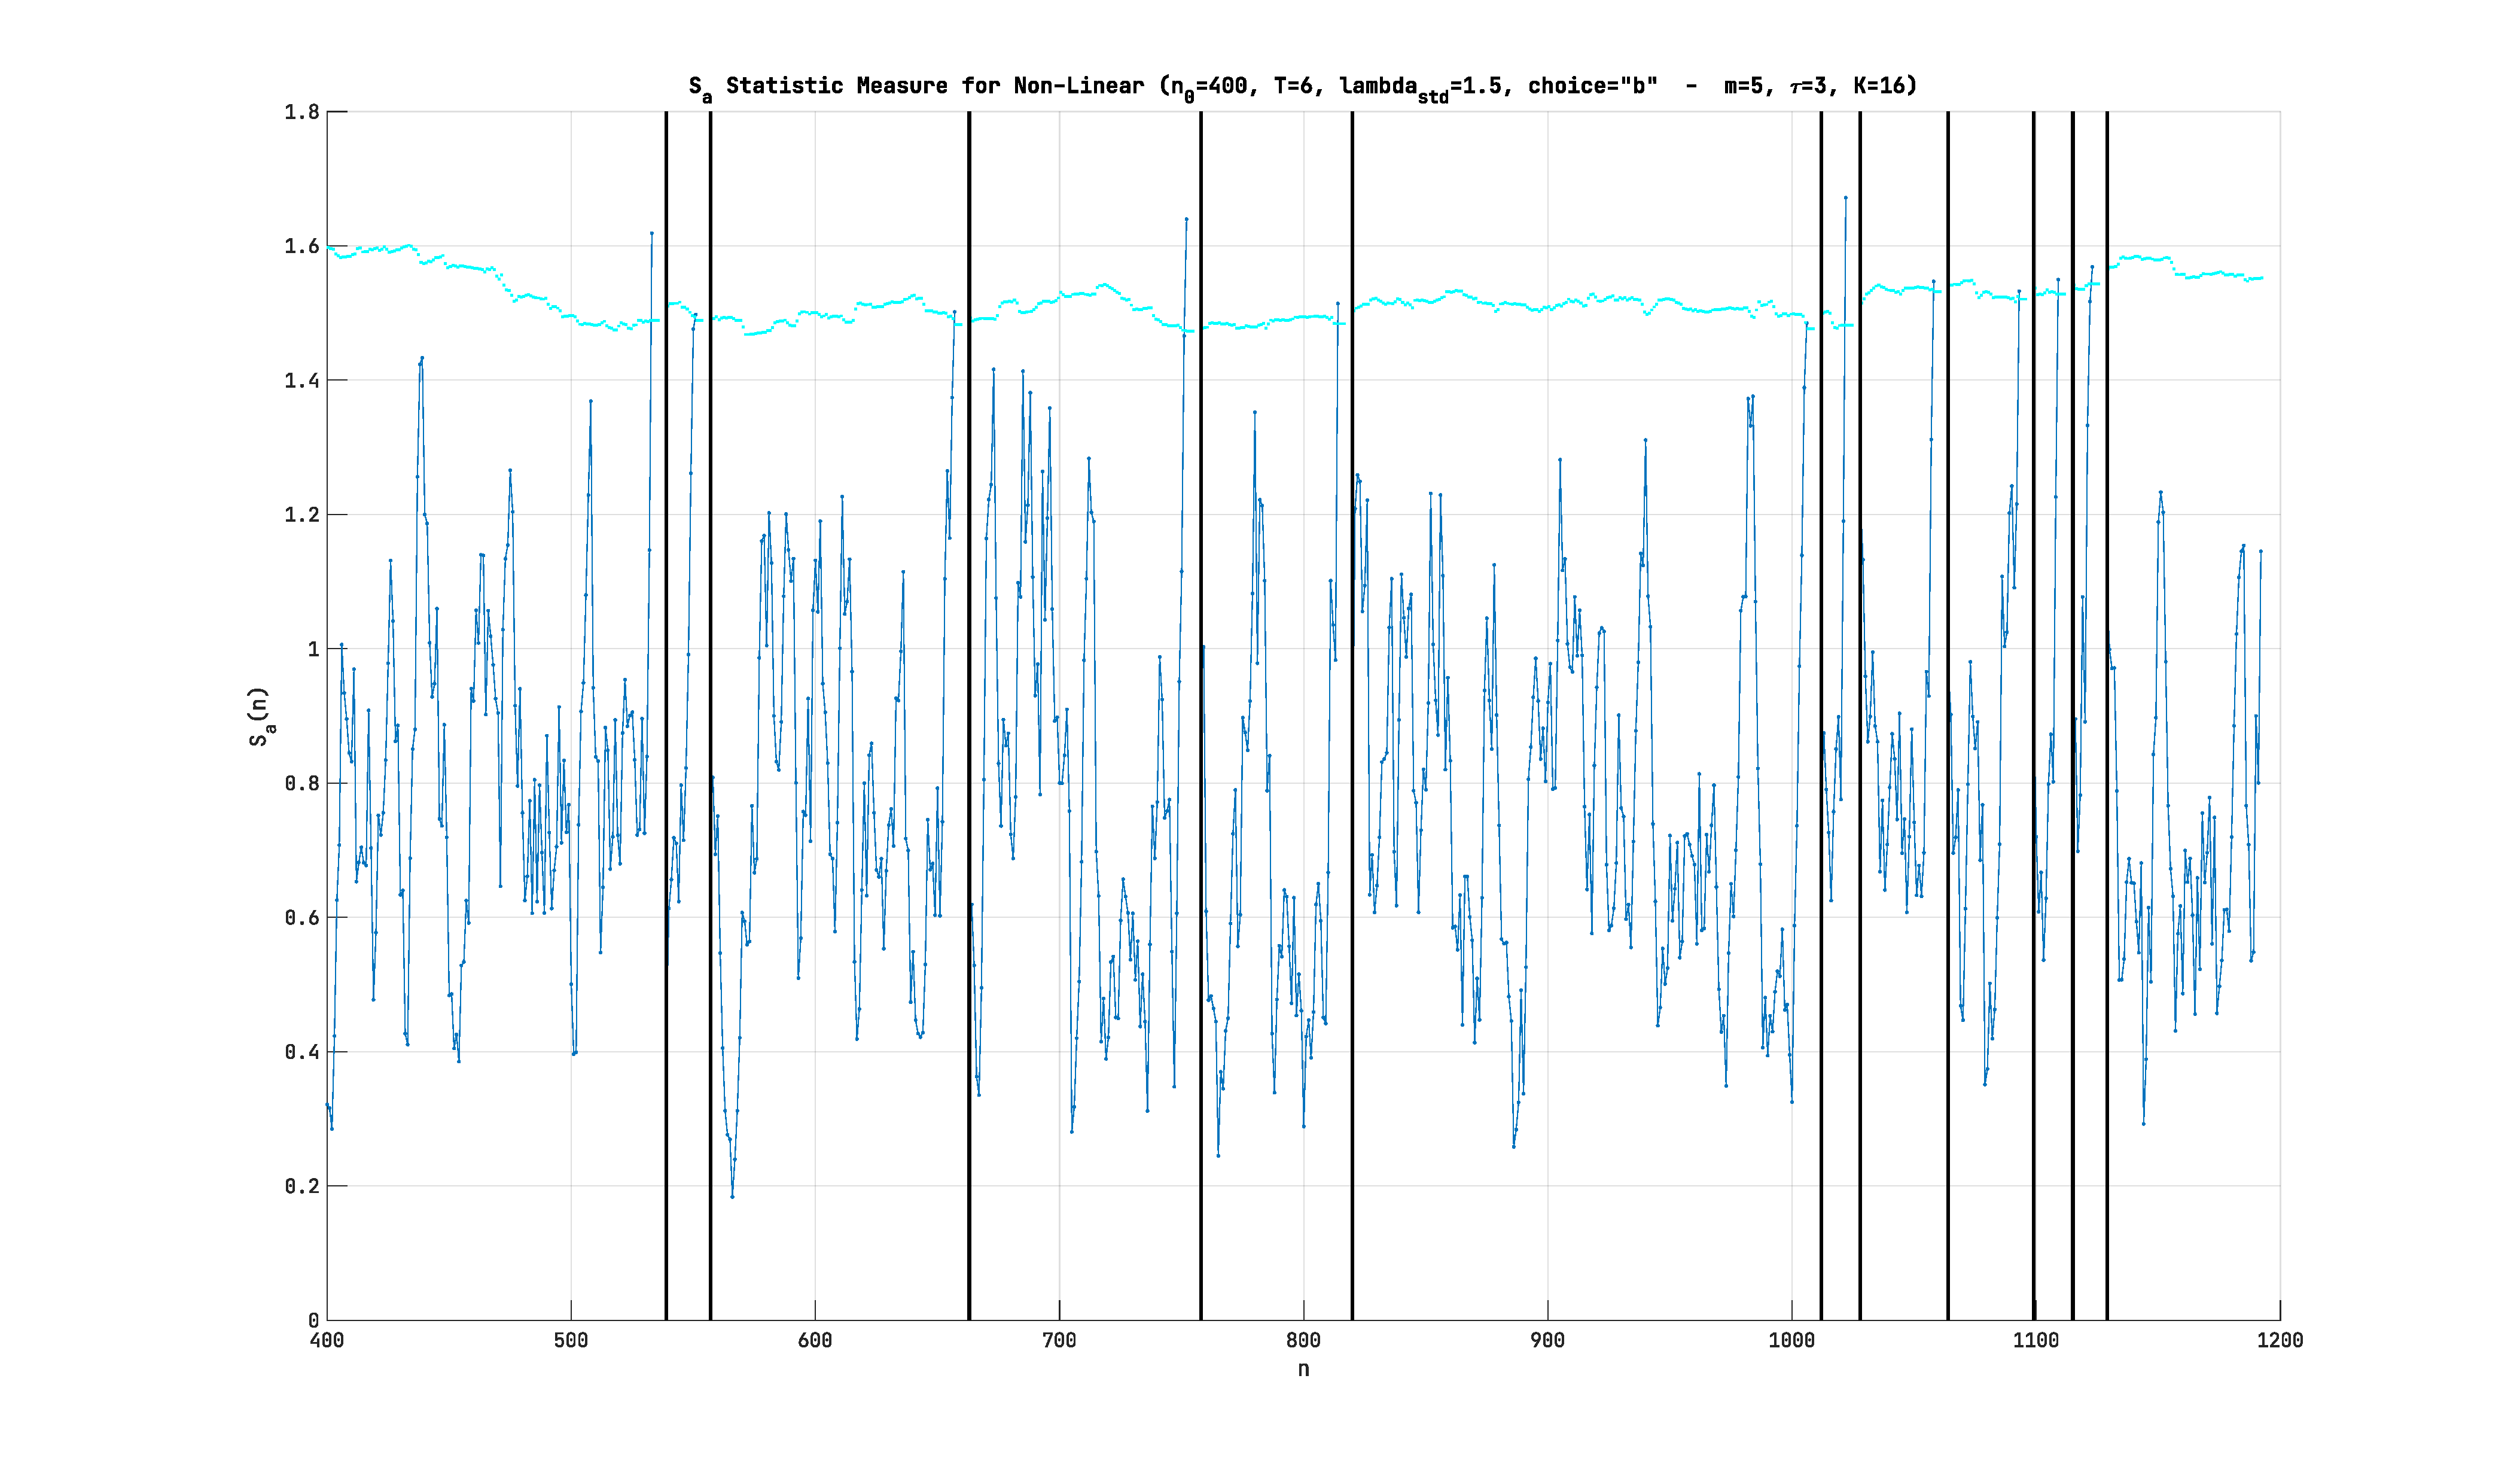
\includegraphics[width=\textwidth]{plots/mcps_nl_xa_opt_b.svg.pdf}
        \caption{Τιμές στατιστικού $S_n$ για έως και 6 βήματα μπροστά πρόβλεψη με τοπική πρόβλεψη μέσου Κ=16 κοντινότερων γειτόνων της στάσιμης χρονοσειράς $\{X_a(t)\}$ και για επιλογή αναπροσαρμογής \textquote{\tl{b}} (αναπροσαρμογή σε κάθε χρονική στιγμή). Σημειώνονται επίσης το κριτήριο απόφασης, $\alpha=1.5*s_x$, (\tl{cyan}) και φυσικά τα σημεία αλλαγής με έντονες κάθετες γραμμές στα εκάστοτε σημεία $n+T$ (μαύρο) - [\tl{NRMSE}=0.934, \ 0.62\tl{sec}]}
        \label{fig:mcps_nl_xa_opt_b}
    \end{center}
\end{figure}

Παρακάτω, τα ίδια σημεία αλλαγής απεικονίζονται στην αρχική χρονοσειρά προβολών του βίντεο \tl{A}:

\begin{figure}[H]
    \begin{center}
        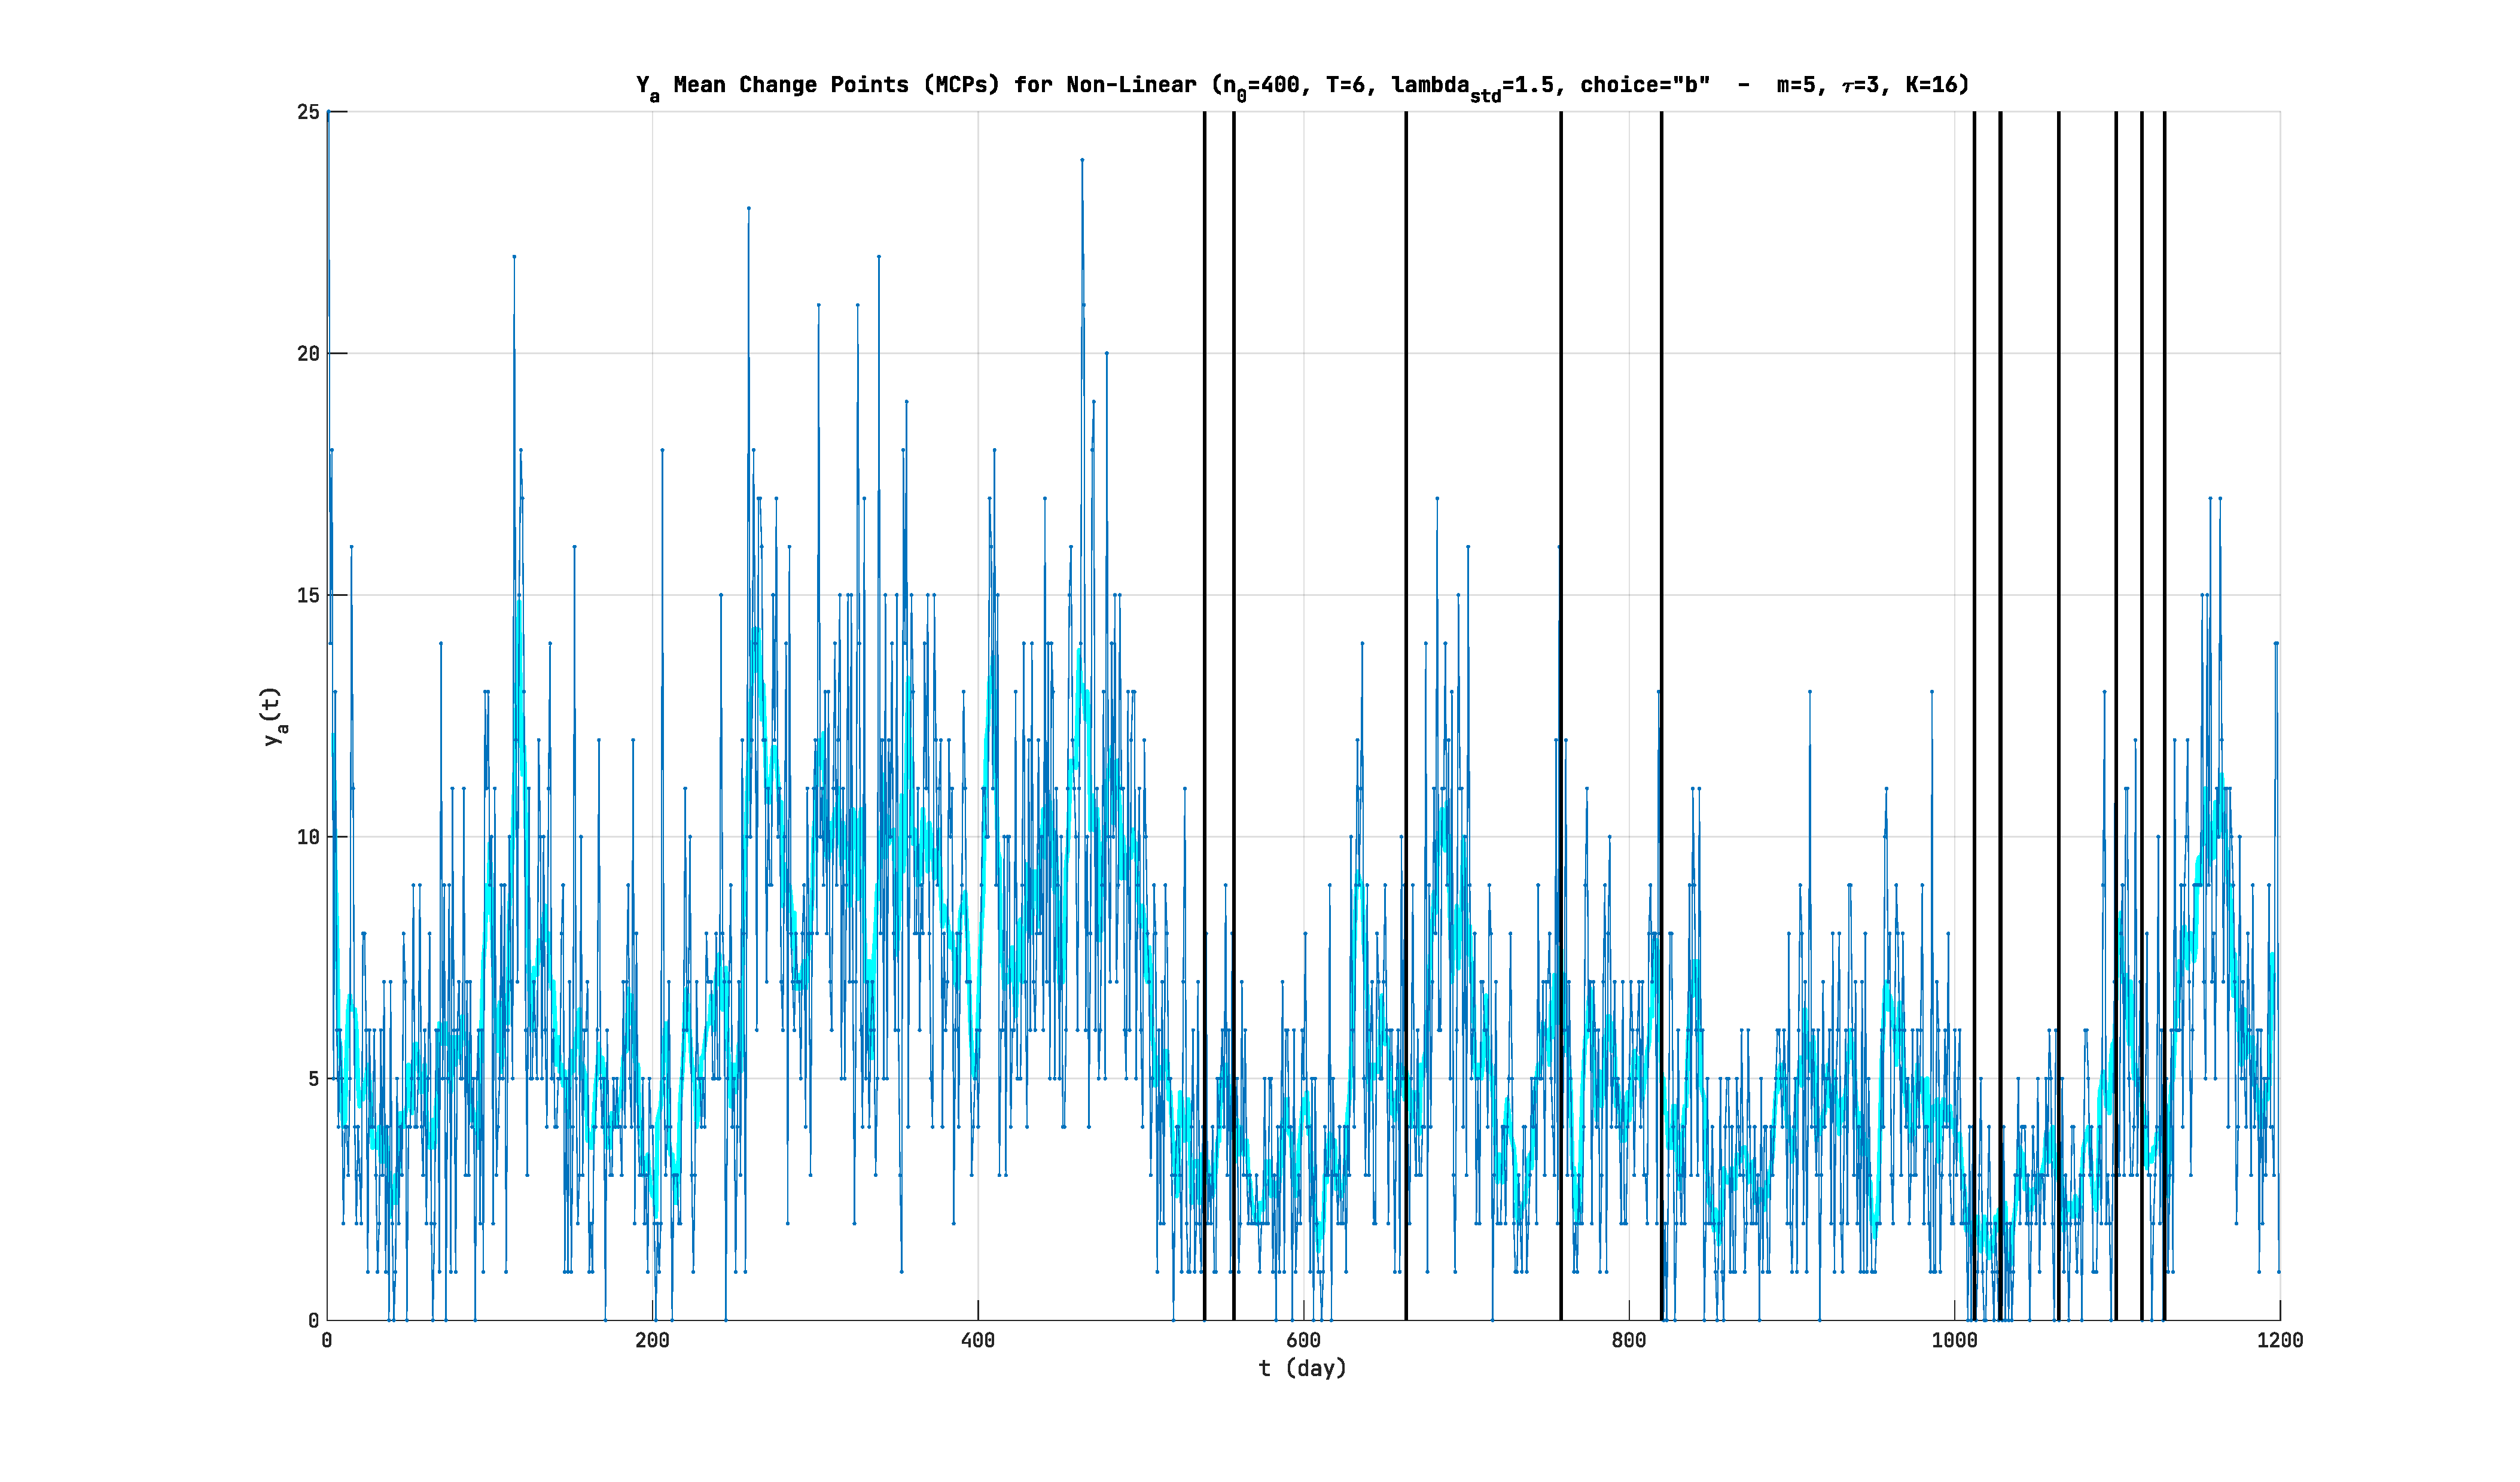
\includegraphics[width=\textwidth]{plots/mcps_nl_ya_opt_b.svg.pdf}
        \caption{Διάγραμμα ιστορίας της αρχικής χρονοσειράς $\{Y_a(t)\}$ (μπλε) μαζί με τα σημεία αλλαγής (μαύρο) που επιλέχθηκαν από τη μη-γραμμική ανάλυση της στάσιμης εκδοχής της με τις βέλτιστες παραμέτρους, καθώς και εκτίμηση της τάσης με φίλτρο κινούμενου μέσου τάξης 7 ($MA(7)$ \tl{smoothing}) - επιλογή \textquote{\tl{b}}}
        \label{fig:mcps_nl_ya_opt_b}
    \end{center}
\end{figure}

Φαίνεται η κυμάτωση του ορίου απόφαση καθώς αυτό επαναϋπολογίζεται σε κάθε χρονική στιγμή. Επίσης, βλέπουμε πως έχουν βγει ακόμα τρία σημεία αλλαγής λόγω αυτής της μεταβολής και πλέον είναι 11 (ενώ πριν ήταν 8). Επίσης υπάρχει μικρή αύξηση του \tl{NRMSE}.

\paragraph{Χωρίς Αναπροσαρμογή}- Επιλογή \textquote{\tl{a}}

Τέλος, τα ίδια διαγράμματα παρουσιάζονται για την επιλογή αναπροσαρμογής \textquote{\tl{a}} (καμία αναπροσαρμογή - διατήρηση της τυπικής απόκλισης / ορίου απόφασης που υπολογιστήκε από τις πρώτες 400 παρατηρήσεις της στάσιμης χρονοσειράς), ενώ ακολουθεί σύντομος σχολιασμός:

\begin{figure}[H]
    \begin{center}
        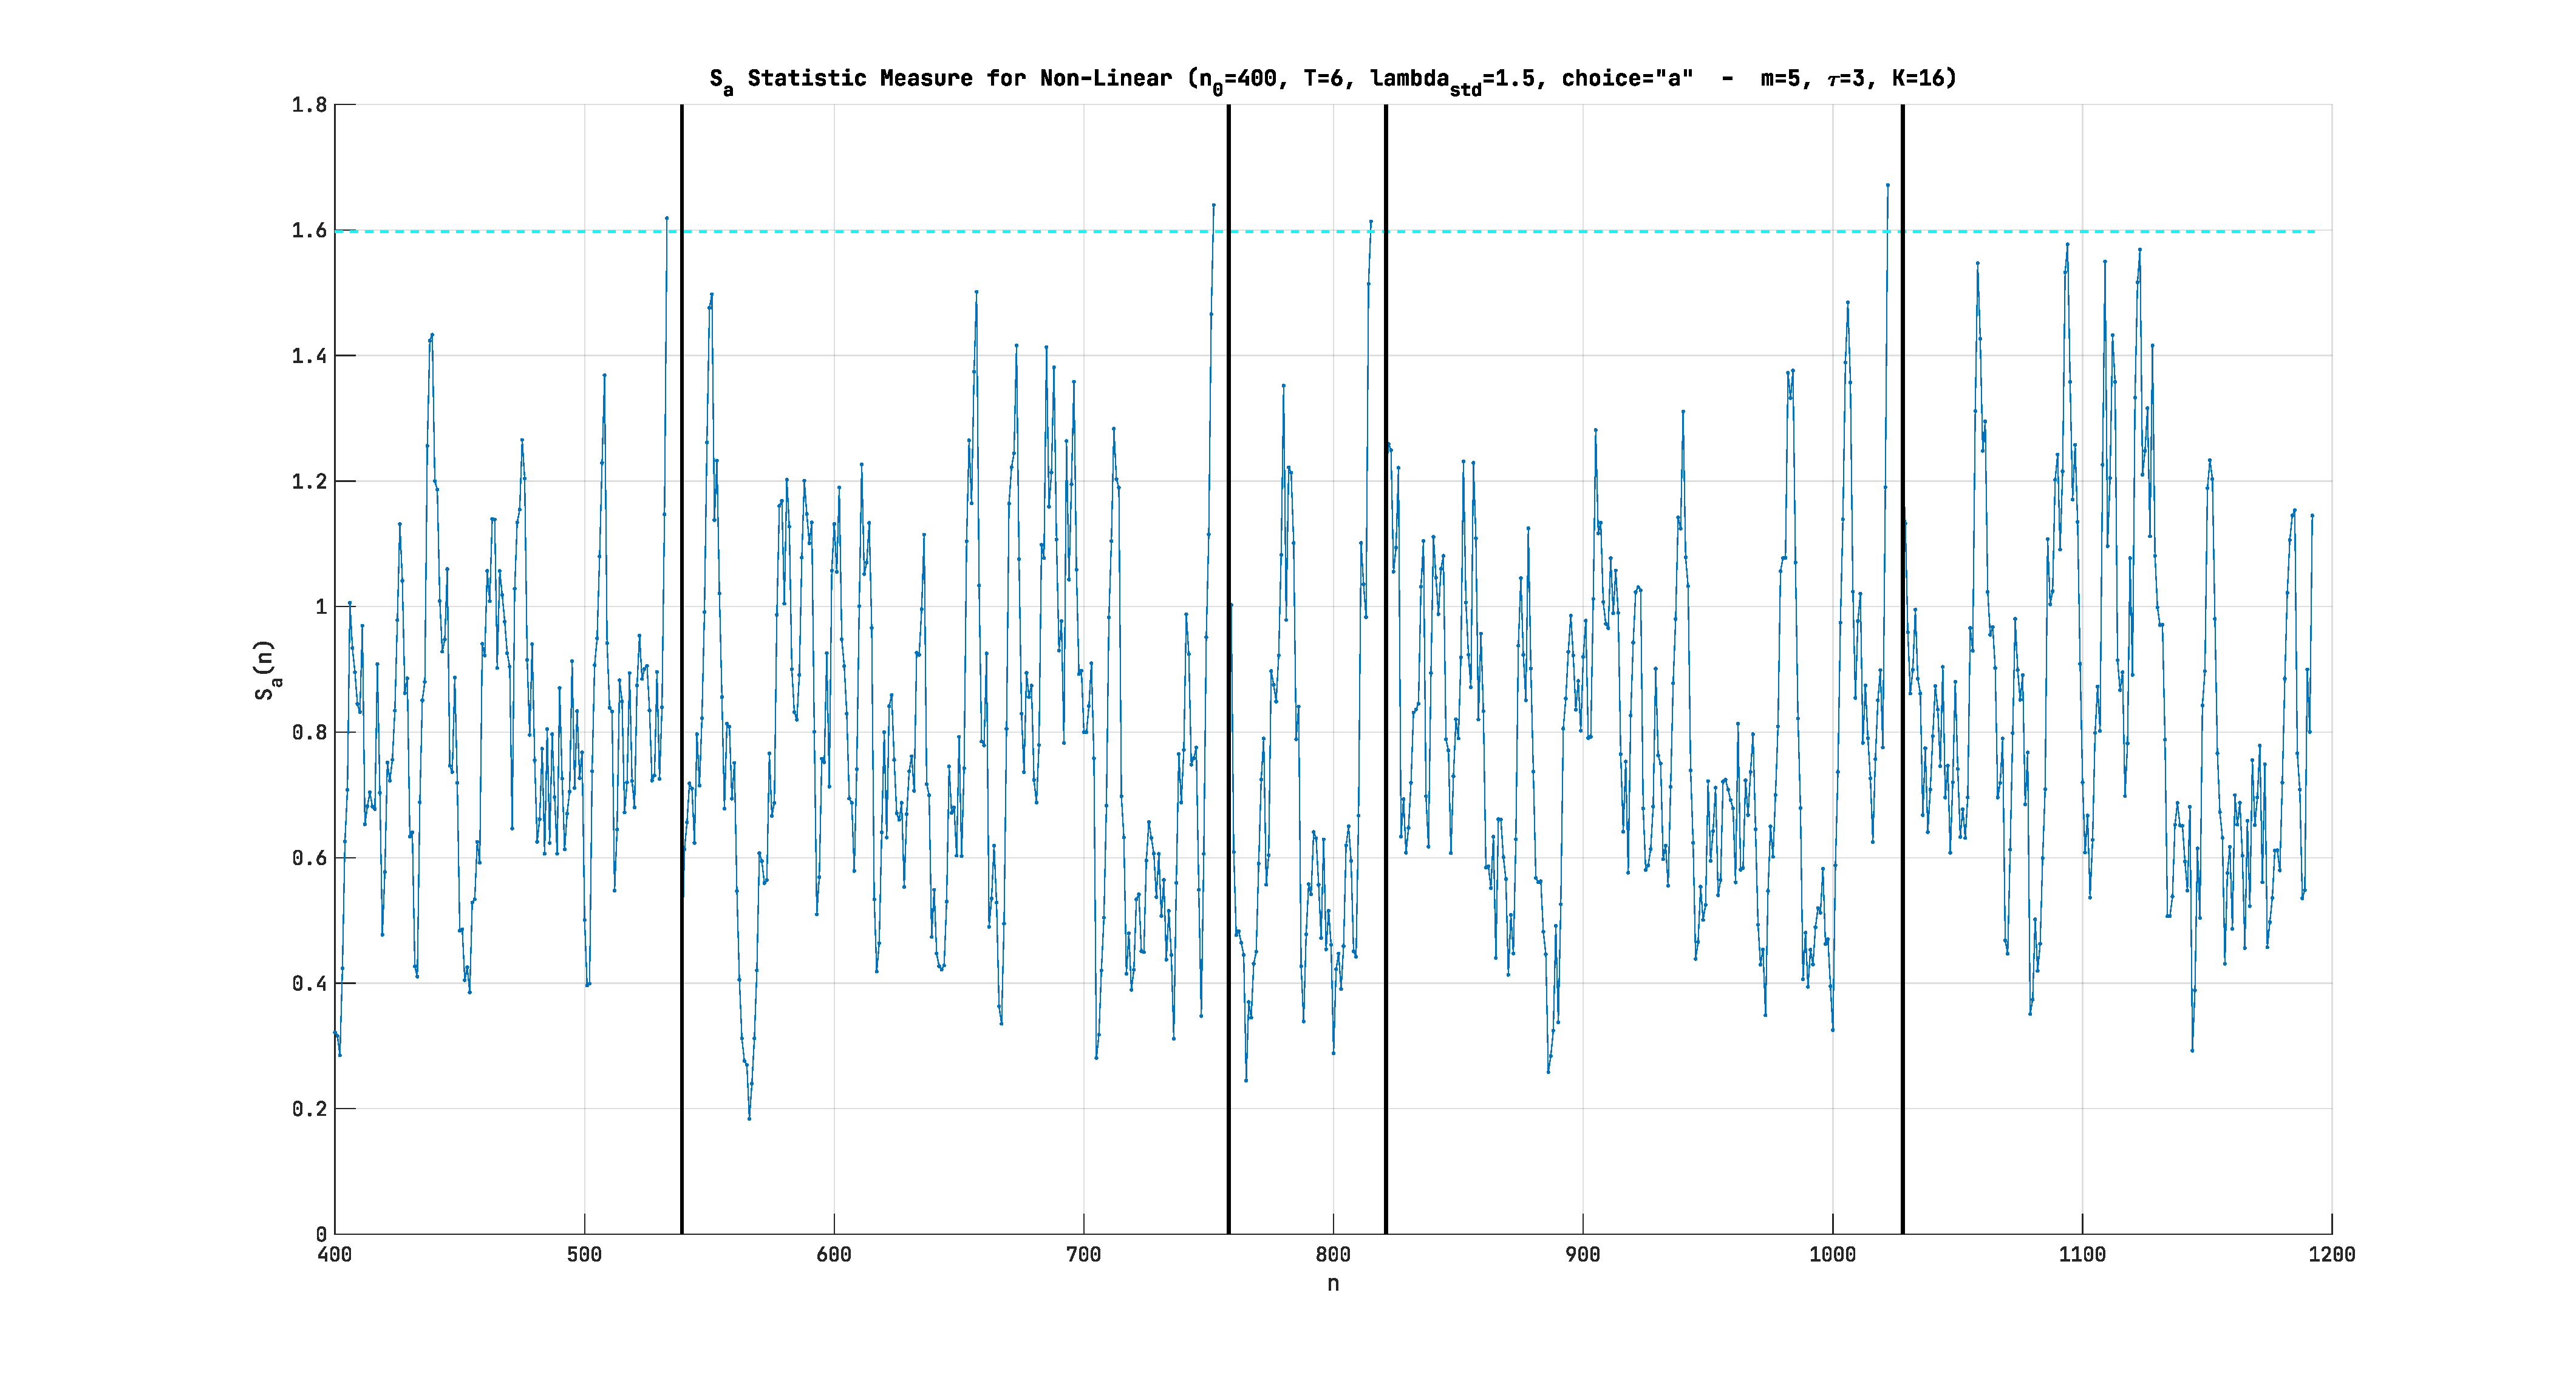
\includegraphics[width=\textwidth]{plots/mcps_nl_xa_opt_a.svg.pdf}
        \caption{Τιμές στατιστικού $S_n$ για έως και 6 βήματα μπροστά πρόβλεψη με τοπική πρόβλεψη μέσου Κ=16 κοντινότερων γειτόνων της στάσιμης χρονοσειράς $\{X_a(t)\}$ και για επιλογή αναπροσαρμογής \textquote{\tl{a}} (χωρίες αναπροσαρμογή). Σημειώνονται επίσης το κριτήριο απόφασης, $\alpha=1.5*s_x$, (\tl{cyan}) και φυσικά τα σημεία αλλαγής με έντονες κάθετες γραμμές στα εκάστοτε σημεία $n+T$ (μαύρο) - [\tl{NRMSE}=0.910, \ 0.61\tl{sec}]}
        \label{fig:mcps_nl_xa_opt_a}
    \end{center}
\end{figure}

Παρακάτω, τα ίδια σημεία αλλαγής απεικονίζονται στην αρχική χρονοσειρά προβολών του βίντεο \tl{A}:

\begin{figure}[H]
    \begin{center}
        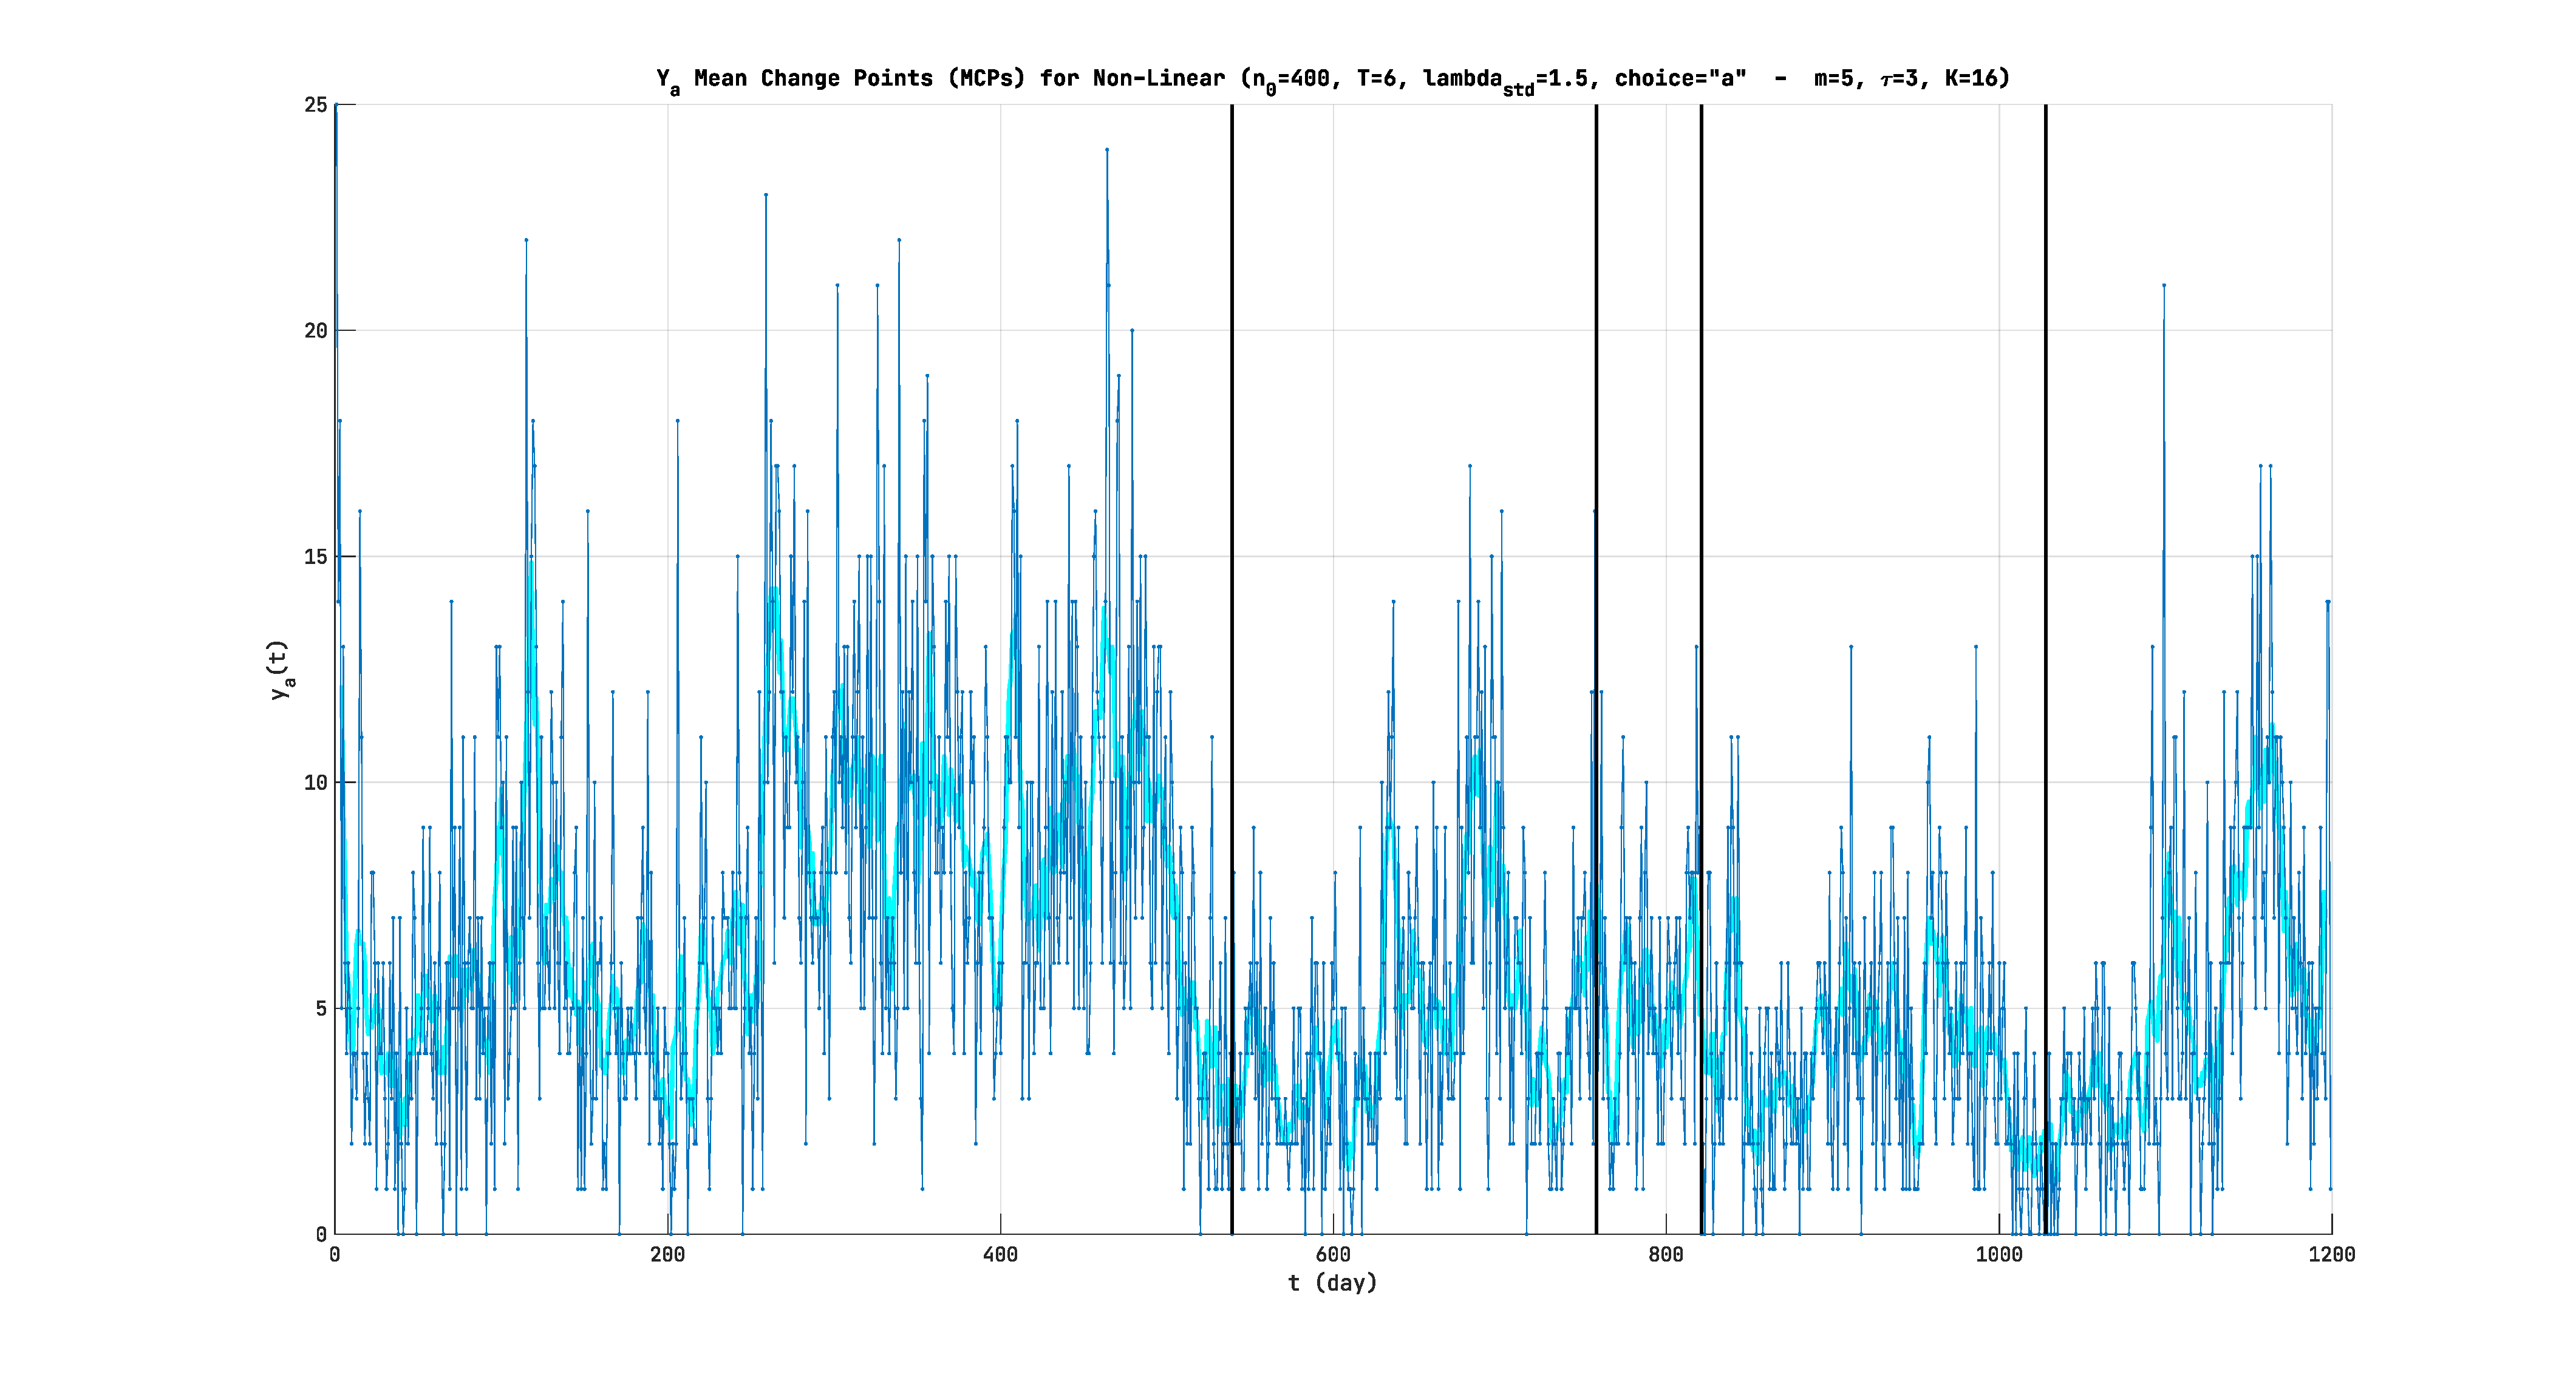
\includegraphics[width=\textwidth]{plots/mcps_nl_ya_opt_a.svg.pdf}
        \caption{Διάγραμμα ιστορίας της αρχικής χρονοσειράς $\{Y_a(t)\}$ (μπλε) μαζί με τα σημεία αλλαγής (μαύρο) που επιλέχθηκαν από τη μη-γραμμική ανάλυση της στάσιμης εκδοχής της με τις βέλτιστες παραμέτρους, καθώς και εκτίμηση της τάσης με φίλτρο κινούμενου μέσου τάξης 7 ($MA(7)$ \tl{smoothing}) - επιλογή \textquote{\tl{a}}}
        \label{fig:mcps_nl_ya_opt_a}
    \end{center}
\end{figure}

Τα σημεία αλλαγής είναι πολύ λιγότερα σε αριθμό και σε άλλες θέσεις σε σχέση με αυτά της επιλογής \textquote{\tl{c}}. Ο χρονος εκτέλεσης είναι ίδιος και το αλλά \tl{NRMSE} αρκετά καλύτερο. 

\par \textit{Γενικότερα όσο μειώνονται τα σημεία αλλαγής που βγάζει η μέθοδος (μέχρι καποιο σημείο) τόσο και το \tl{NRMSE} των προβλέψεων κατά την εφαρμογή της μεθόδου μειώνεται.\\
Συγκρίνοντας τα σημεία αλλαγής με τα αντίστοιχα από τη γραμμική πρόβλεψη και ανάλυση του βήματος \ref{ch:step4} βλέπουμε ότι \textbf{υπάρχει σχετική συνέπεια} στις θέσεις όπου εντοπίζονται σημεία αλλαγής, δηλαδή γύρω από τοπικες \textquote{εξάρσεις} ή τοπικές \textquote{βυθίσεις} της αρχικής χρονοσειράς προβολών του βίντεο A. Ωστόσο, επειδή \textbf{η επιλογή σημείων αλλαγής με γραμμικό μοντέλο πρόβλεψης} αφήνει μικρότερο \tl{NRMSE}, θα λέγαμε πως \textbf{υπερτερεί} έναντι της χρήσης μη-γραμμικού τοπικού μοντέλου κοντινότερων γειτόνων.}


%----------------------------------------------------------------------


\subsection{Εφαρμογή στη στάσιμη χρονοσειρά Β}

Για να τρέξει το \tl{grid search} θέτουμε τη τιμή \textbf{\tl{K}=13 κοντινότερους γείτονες} σύμφωνα με τη τιμή που προέκυψε από το σχήμα \ref{fig:nrmse_k_b}.

\subsubsection{Επιλογή Βέλτιστων Παραμέτρων}

Για επιλογή βέλτιστων τιμών στις \tl{hyperparameters} της μεθόδου και συγκεκριμένα στον ορίζοντα πρόβλεψης, $T$, και στο $\lambda_{std}$ του ορίου απόφασης, $\alpha$, θα κάνουμε και πάλι αναζήτηση πλέγματος ως προς αυτές. Ως μετρικές για αξιολόγηση του κάθε συνδυασμού των παραμέτρων αυτών χρησιμοποιήθηκαν και εδώ ο \textit{Αριθμός των σημειών αλλαγής \tl{MCPs}} και το \textit{\tl{NRMSE} των προβλέψεων}.

Αρχικά παραθέτονται σε διαγράμματα τύπου \tl{surf} τα αποτελέσματα αναζήτησης πλέγματος ως προς τις παραπάνω μετρικές για τη στάσιμη χρονοσειρά $\{X_{b_{deseasoned}}(t)\}$, ενώ στη συνέχεια σχολιάζεται ο τρόπος επιλογής προσεγγεστικά βέλτιστων παραμάτρων αλλά και οι τελικές τους τιμές.

\begin{figure}[H]
    \begin{center}
        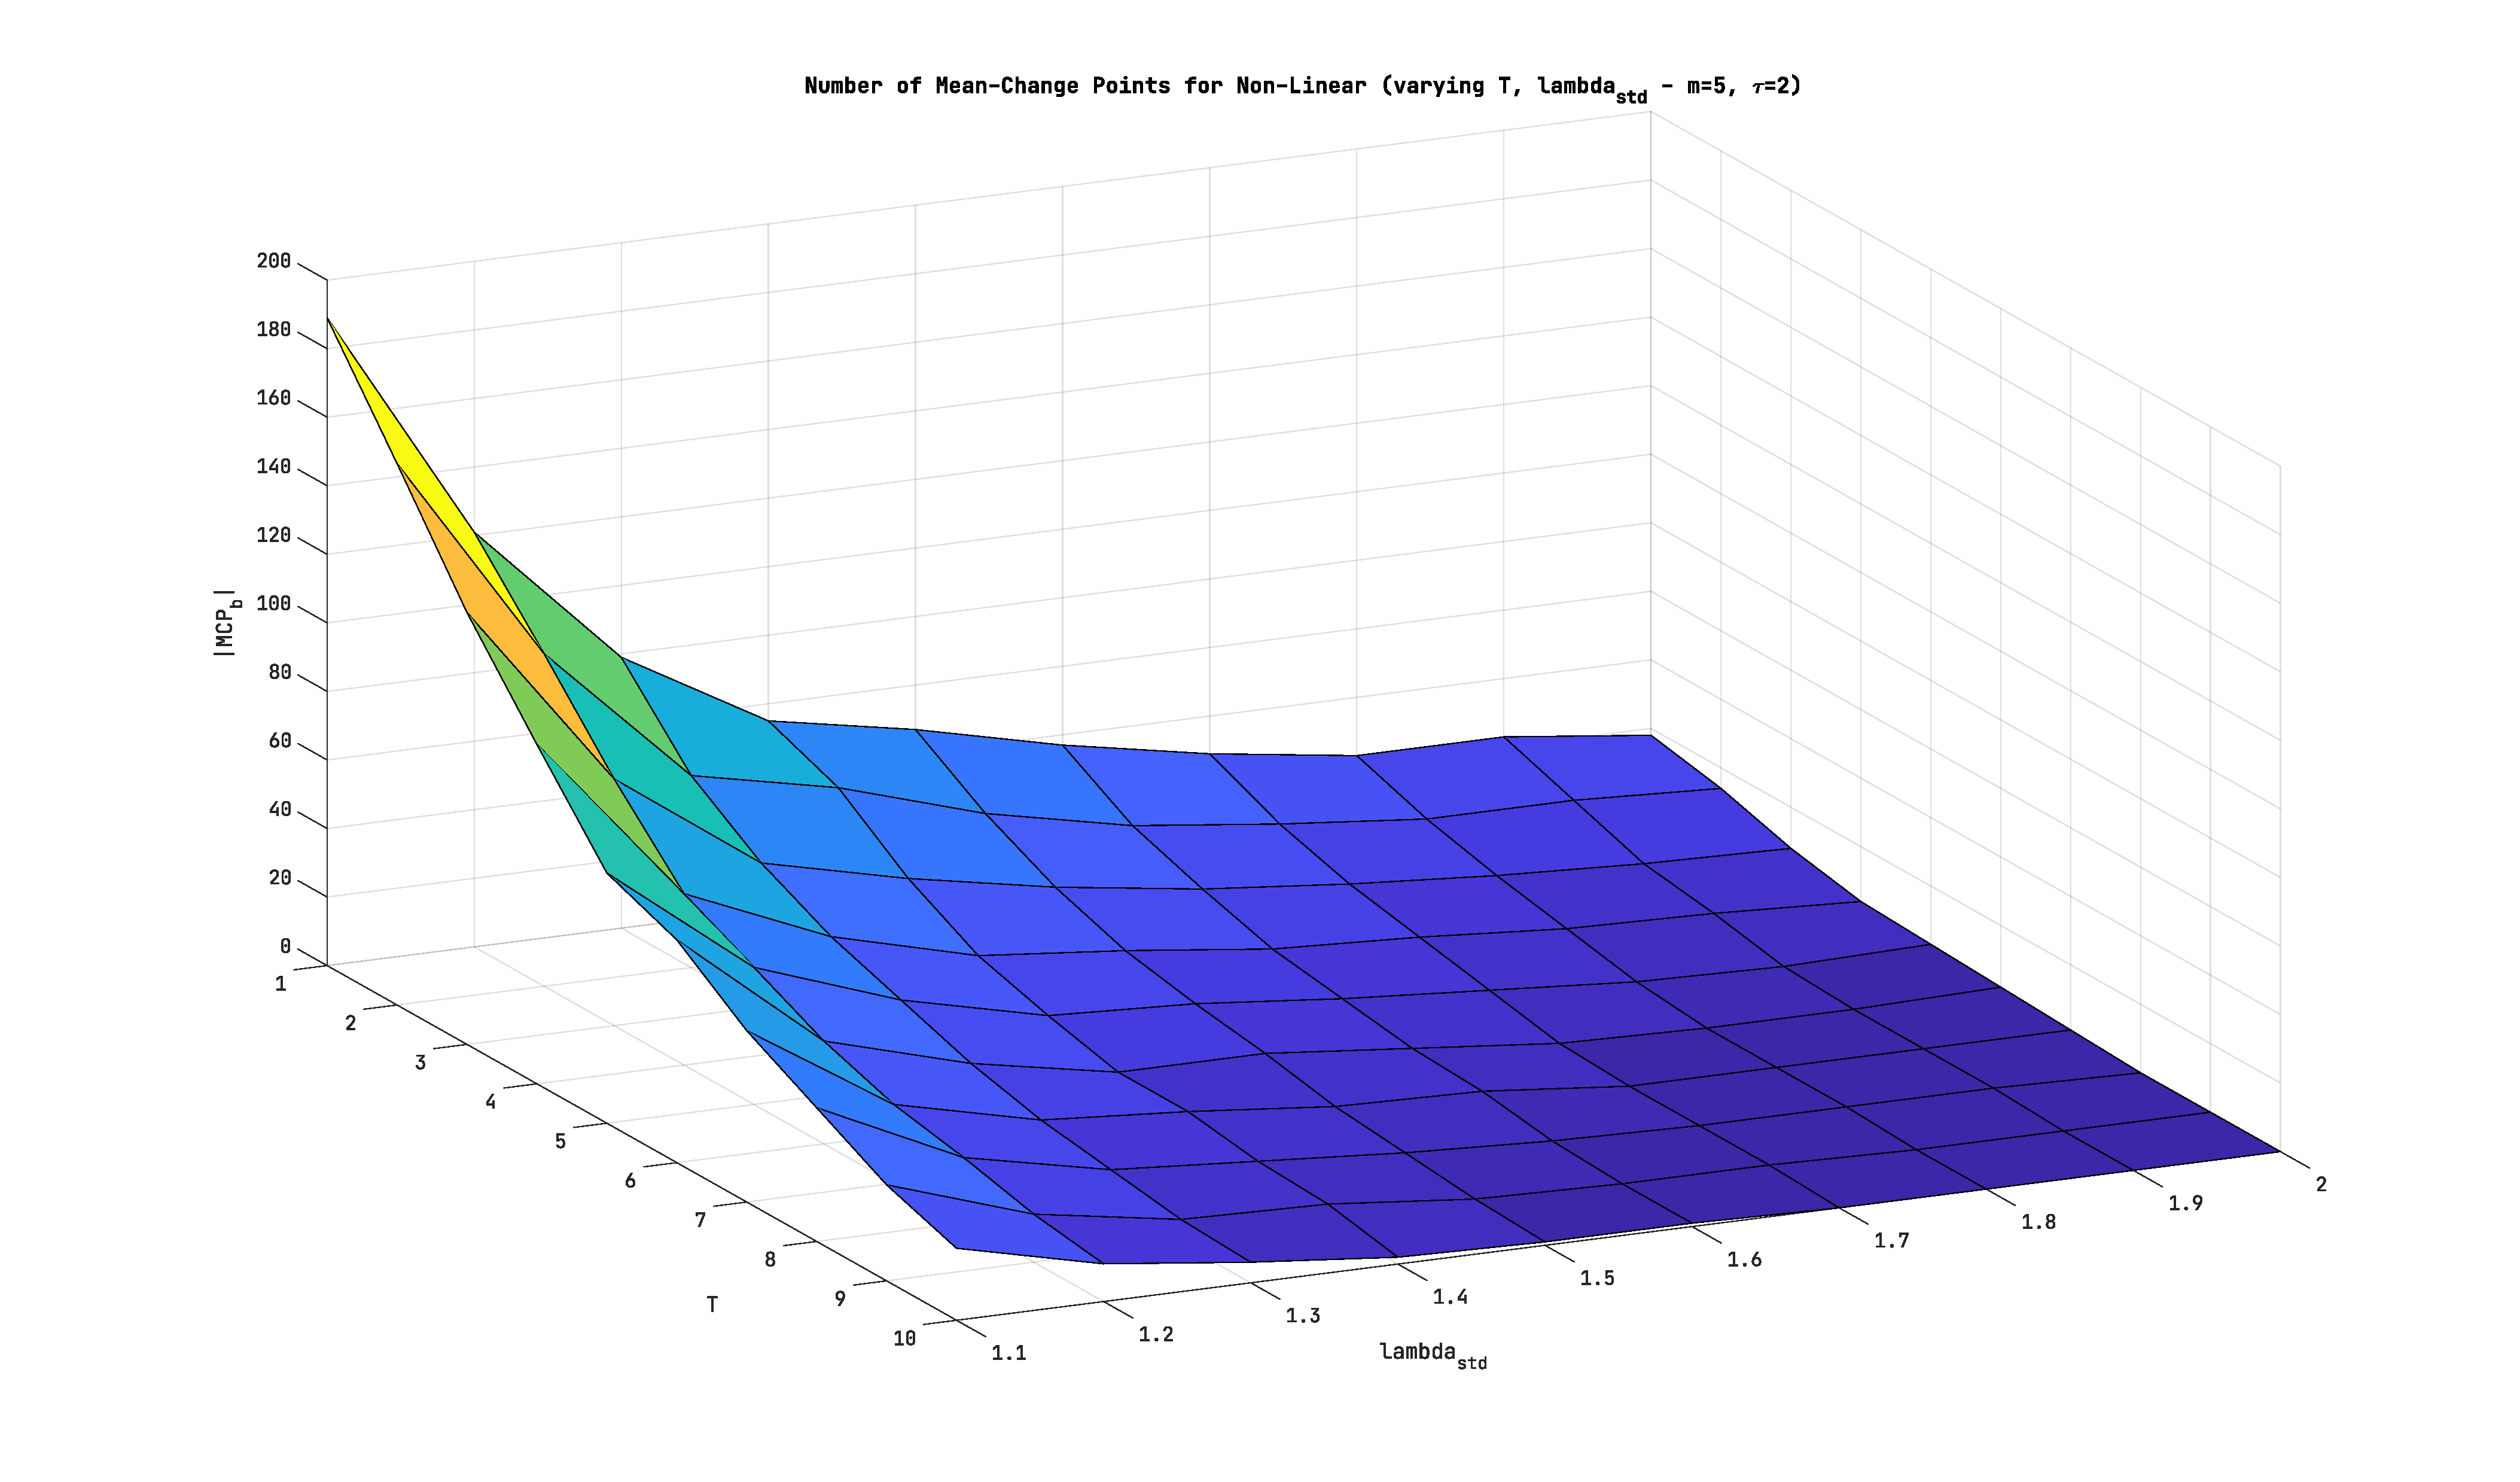
\includegraphics[width=\textwidth]{assets/images/plots/mcps_count_nl_b.svg.pdf}
        \caption{Αριθμός σημείων αλλαγής της στάσιμης χροσνοσειράς Β, $\vert$\tl{MCP}$\vert$, που προκύπτουν για κάθε τιμή του πλέγματος αναζήτησης ως πρός τον ορίζοντα πρόβλεψης, $T$, και το $\lambda_{std}$ του ορίου απόφασης, $\alpha$, για παραμέτρους μη-γραμμικού μοντέλου $m=5$, $\tau=2$ και $K=13$}
        \label{fig:mcps_count_nl_b}
    \end{center}
\end{figure}

\begin{figure}[H]
    \begin{center}
        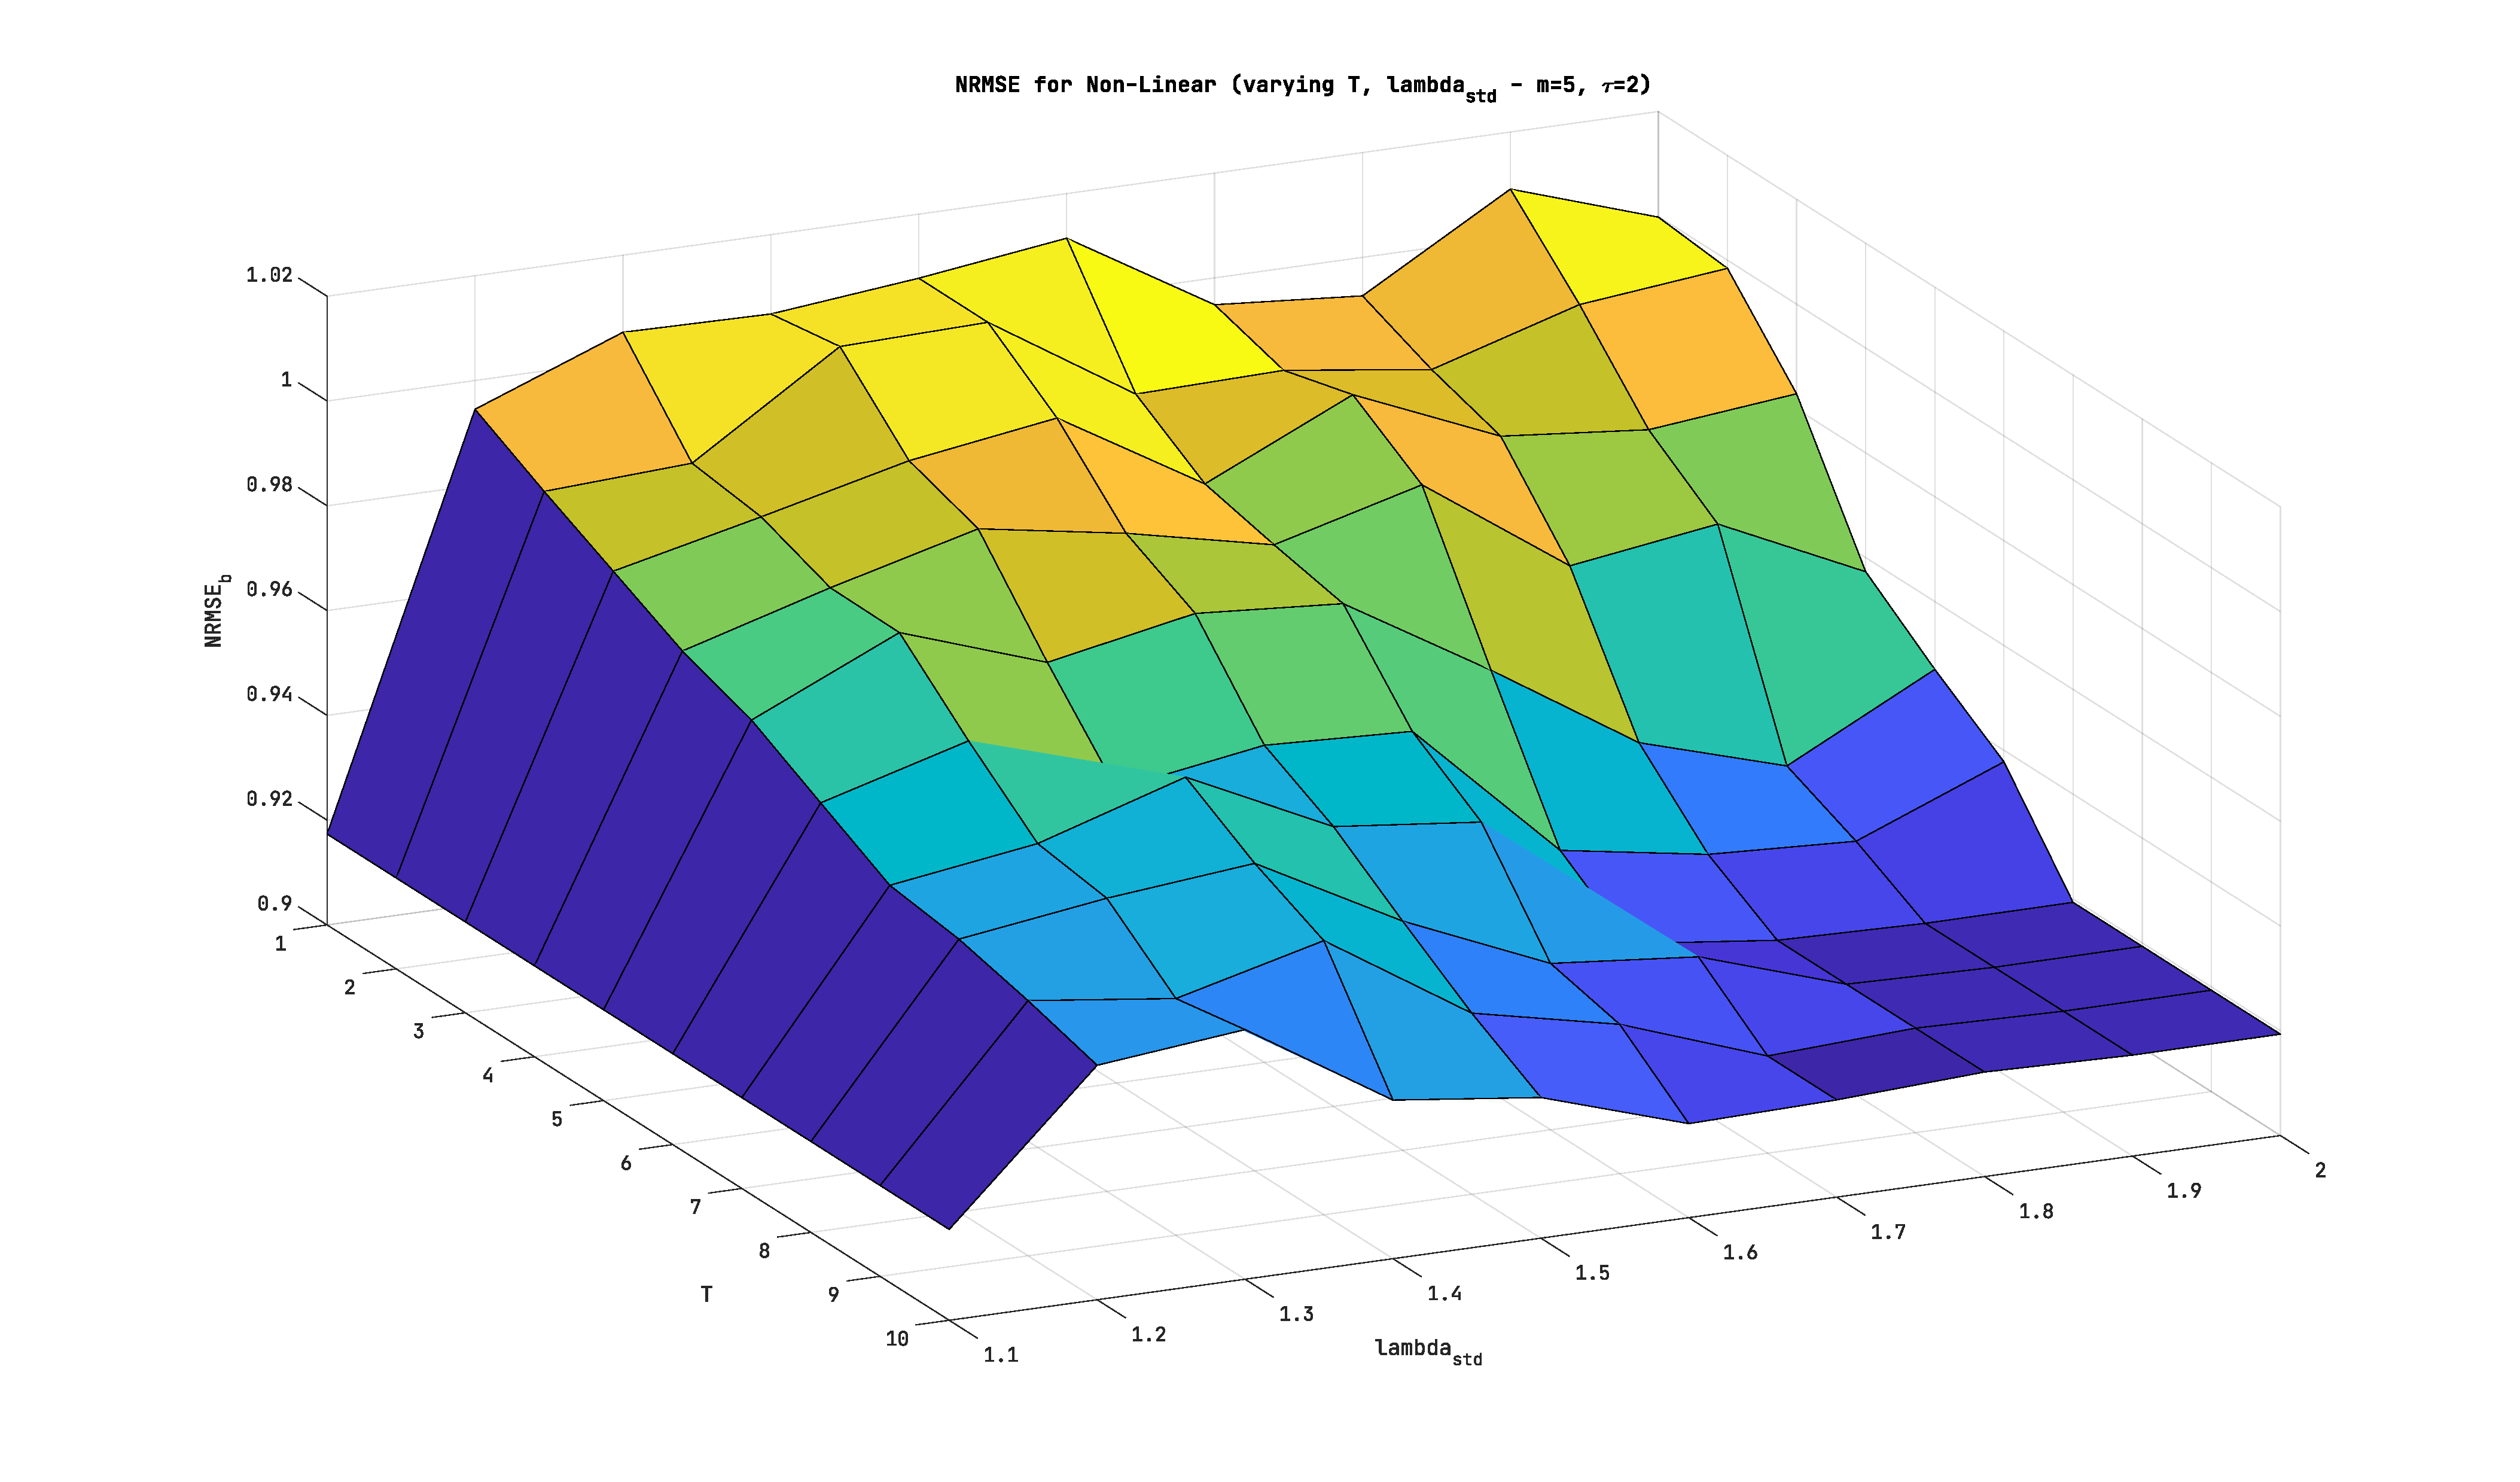
\includegraphics[width=\textwidth]{plots/nrmse_nl_b.svg.pdf}
        \caption{\tl{NRMSE} προβλέψεων κατά τον υπολογισμό των σημείων αλλαγής (\tl{MCPs}) της στάσιμης χροσνοσειράς Β, για κάθε τιμή του πλέγματος αναζήτησης ως πρός τον ορίζοντα πρόβλεψης, $T$, και το $\lambda_{std}$ του ορίου απόφασης, $\alpha$, για παραμέτρους μη-γραμμικού μοντέλου $m=5$, $\tau=2$ και $K=13$}
        \label{fig:nrmse_nl_b}
    \end{center}
\end{figure}

\par Γενικότερα, αναζητούμε τα \textquote{γόνατα} στις αντίστοιχες τρισδιάστατες καμπύλες έτσι ώστε περαιτέρω μεταβολές των αντίστοιχων παραμέτρων να μην είναι πλέον επικερδείς.

\par Επικεντρώνοντας στο πρώτο διάγραμμα και δεδομένου ότι θέλουμε ο αριθμός των \tl{MCPs} να μήν είναι πολύ μεγάλος ή πολύ μικρός, θα επιλέγαμε τις ακόλουθες τιμές (προσεγγιστικά):
\begin{align}
    T \in [5,9] \ \ \ \& \ \ \ \lambda_{std} \in [1.2, 1.5]
    \label{eq:t_lambda_mcps_nl_b}
\end{align}

\par Επικεντρώνοντας τώρα στο διάγραμμα των \tl{NRMSEs} και δεδομένου ότι θέλουμε το \tl{NRMSE} να είναι κατά το δυνατό μικρό, θα επιλέγαμε τις ακόλουθες τιμές (προσεγγιστικά):
\begin{align}
    T \geq 6 \ \ \ \& \ \ \ \lambda_{std} \geq 1.5
    \label{eq:t_lambda_nrmses_nl_b}
\end{align}

\par Συνδυάζοντας τις σχέσεις (\ref{eq:t_lambda_mcps_nl_b}) και (\ref{eq:t_lambda_nrmses_nl_b}) παραπάνω καταλήγουμε ότι οι \tl{hyperparameters} που θα χρησιμοποιηθούν για την εφαρμογή της μεθόδου αυτόματης εύρεσης χρονικών σημείων αλλαγής θα είναι:
\textbf{T = 6 βήματα} και \textbf{λ\textsubscript{\tl{std}} = 1.5}. Οι αντίστοιχες τιμές του \tl{grid search} είναι: \textbf{$\vert$\tl{MCP}$\vert$ = 9 \tl{MCPs}} και \textbf{\tl{NRMSE} = 0.975}.

\par Η τελική επιλογή παραπάνω έγινε με βάση το μικρότερο \tl{NRMSE} αλλά χωρίς μεγάλη μείωση των \tl{MCPs}. Στη στάσιμη χρονοσειρά Β, οι παράμετροι της μεθόδου δεν ίδιες για τα γραμμικά και μη-γραμμικά μοντέλα, αφού πλέον οι προβλέψεις γίνονται για έως και 6 βήματα εμπρός (σε σύγκριση με τα γραμμικά όπου ήταν για έως 5 βήματα εμπρός). 

\par Για ίδιες παραμέτρους με τις βέλτιστες στη γραμμική ανάλυση θα προέκυπταν 13 \tl{MCPs} (σε σύγκριση με τα 8 στη γραμμική) και \tl{NRMSE} 0.977 (σε σύγκριση με το 0.892).

\textit{Φαίνεται λοιπόν πως και για τη δεύτερη χρονοσειρά, η χρήση του μη-γραμμικού, τοπικού μοντέλου κοντινότερων γειτόνων εμφανίζει μεγαλύτερο \tl{NRMSE} κατά την εφαρμογή της μεθόδου εξαγωγής σημείων αλλαγής σε σύγκριση με τη χρήση γραμμικού μοντέλου}.

\subsubsection{Εφαρμογή Μεθόδου με Βέλτιστες Παράμετρους}

Χρησιμοποιώντας τις επιλεγμένες τιμές για τις \tl{hyperparameters} της μεθόδου, δηλαδή ορίζοντα πρόβλεψης έως και 6 βημάτων εμπρός, $T=6$, παράμετρο ορίου απόφασης στο 1.5, $\lambda_{std}=1.5$, διάσταση εμβύθινσης, $m=5$, υστέρηση, $\tau=2$ και αριθμό κοντινότερων γειτόνων, $K=13$, θα τρέξουμε την παραπάνω μέθοδο στη στάσιμη χρονοσειρά που προέκυψε από το βήμα \ref{ch:step3}, $\{X_{b_{deseasoned}}(t)\}$, κάνοντας προβλέψεις με το μη-γραμμικό τοπικό μοντέλο μέσου όρου. Παρακάτω, φαίνονται τα σημεία αλλαγής που προκύπτουν από την εκτέλεση της μεθόδου με τις παραπάνω παραμέτρους για κάθε μια από τις επιλογές αναπροσαρμογής του μοντέλου (\textquote{\tl{a}}, \textquote{\tl{b}} ή \textquote{\tl{c}}).

\paragraph{Αναπροσαρμογή όταν βρεθεί σημείο αλλαγής}- Επιλογή \textquote{\tl{c}}

\begin{figure}[H]
    \begin{center}
        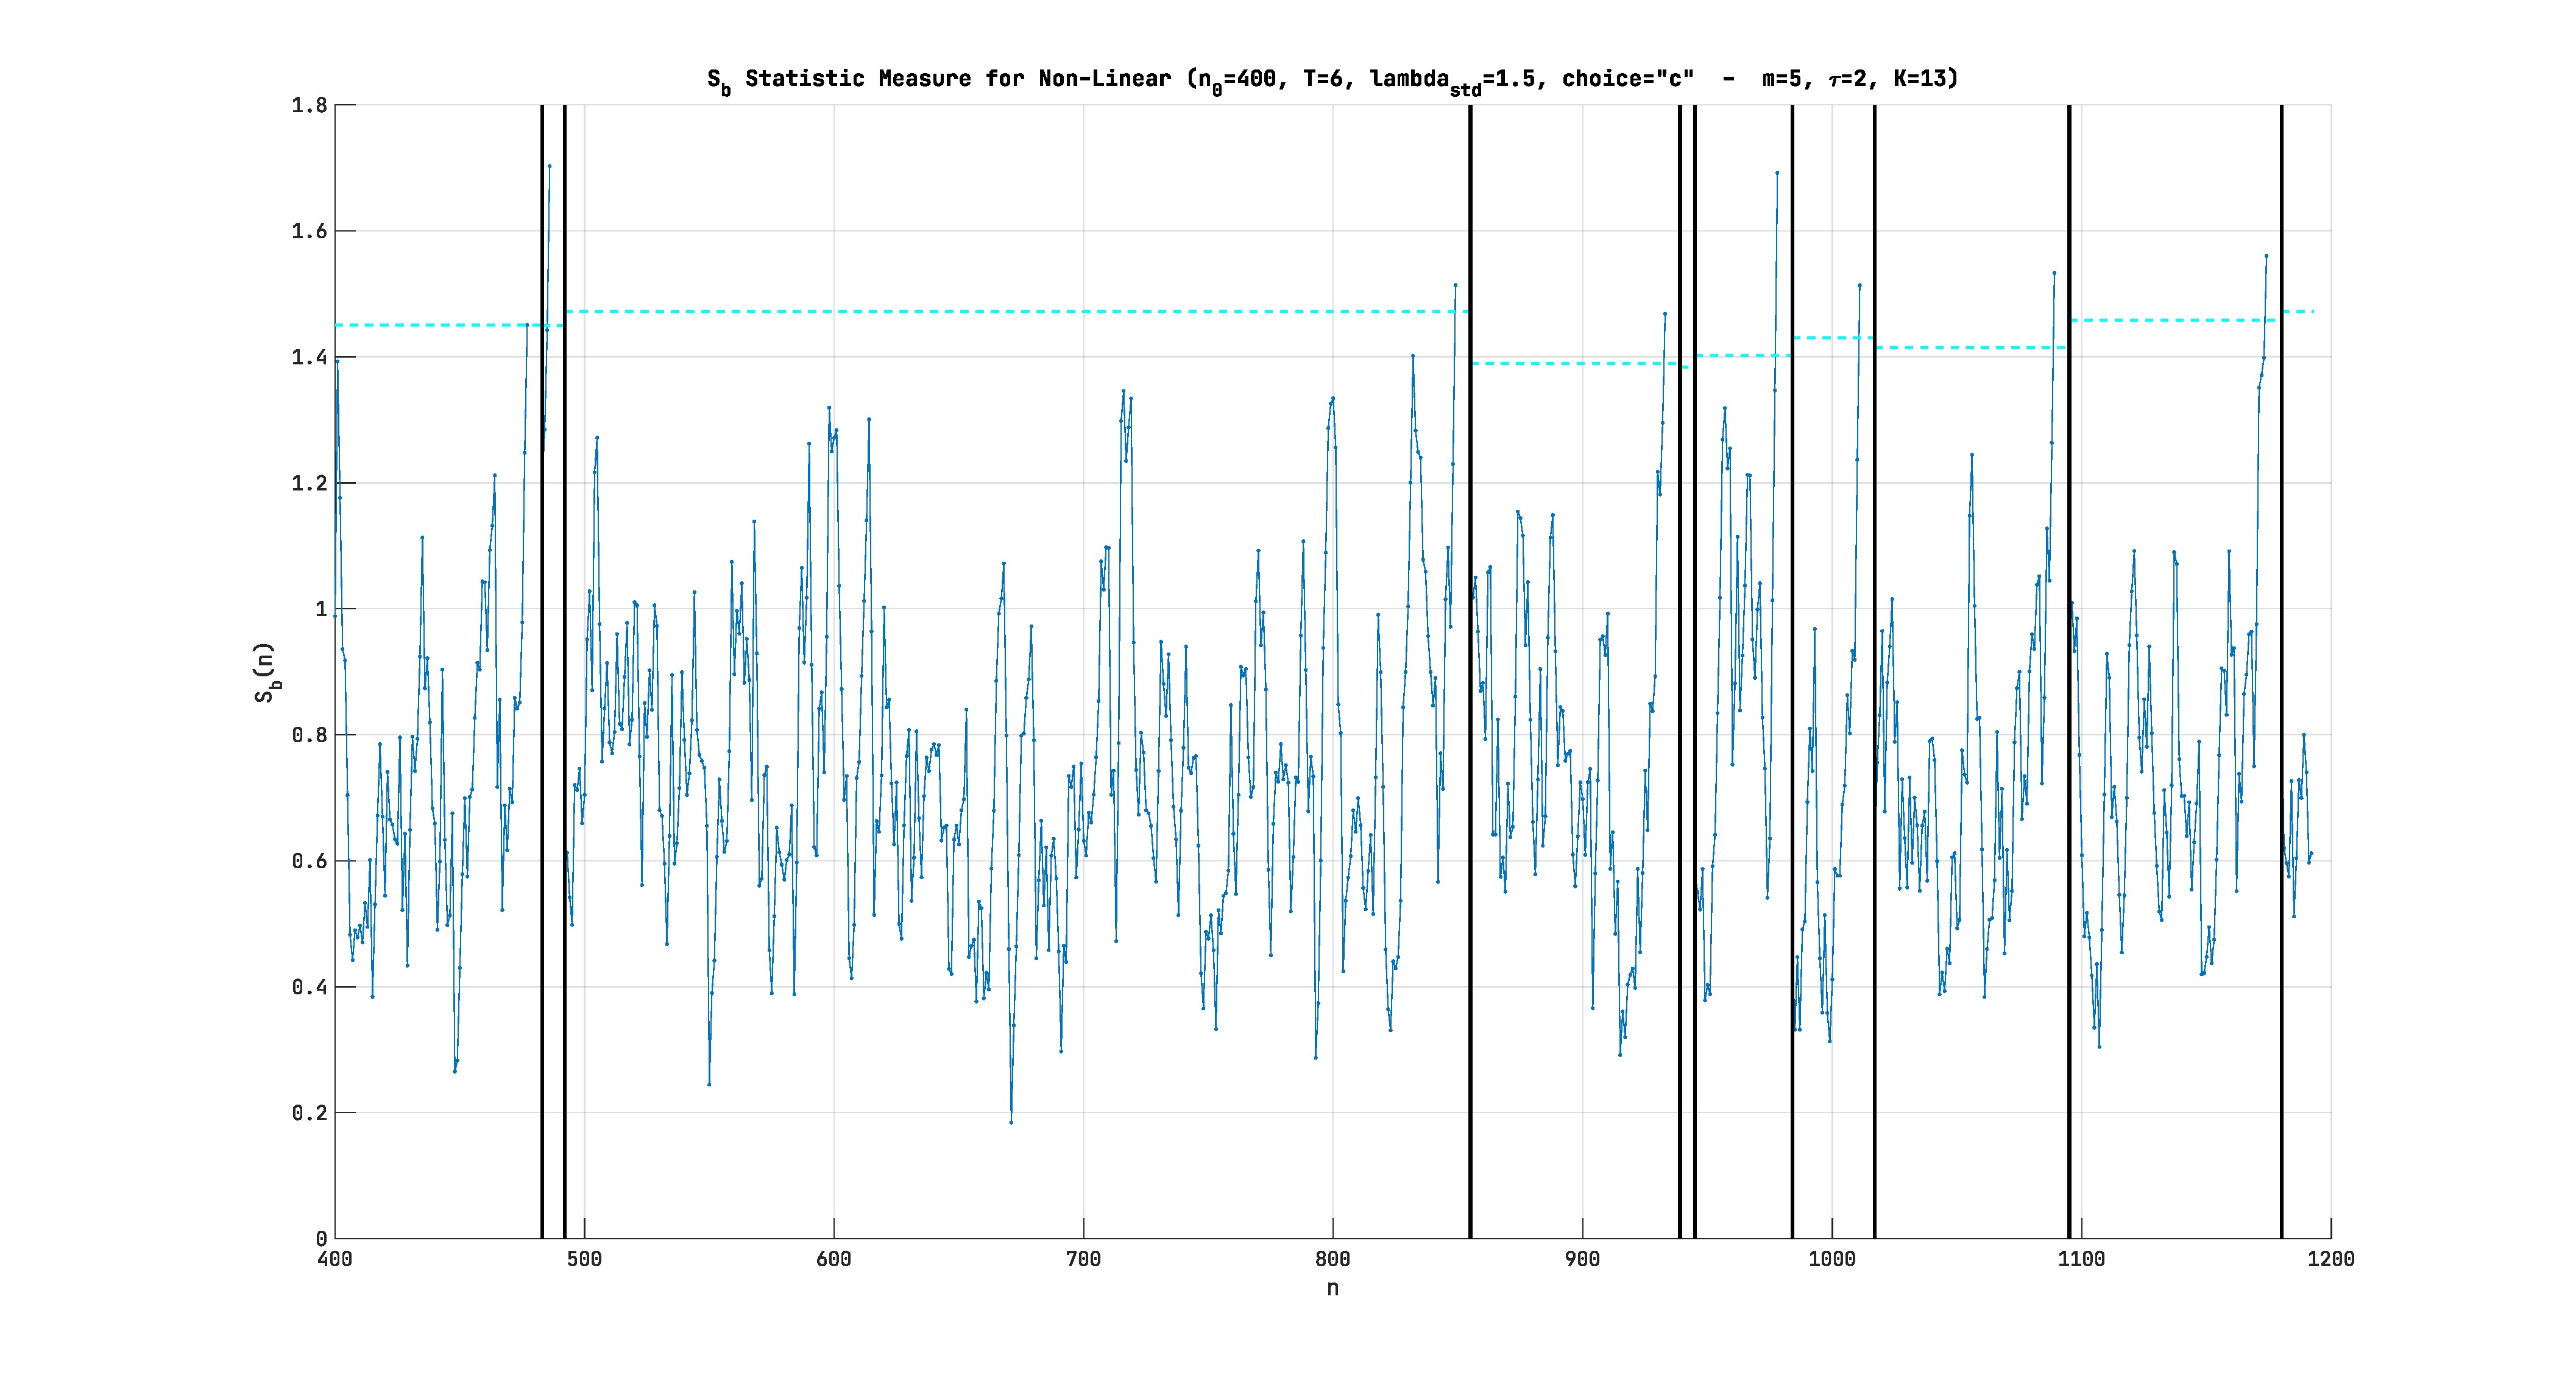
\includegraphics[width=\textwidth]{plots/mcps_nl_xb_opt_c.svg.pdf}
        \caption{Τιμές στατιστικού $S_n$ για έως και 6 βήματα μπροστά πρόβλεψη με τοπική πρόβλεψη μέσου Κ=13 κοντινότερων γειτόνων της στάσιμης χρονοσειράς $\{X_{b_{deseasoned}}(t)\}$ και για επιλογή αναπροσαρμογής \textquote{\tl{c}} (αναπροσαρμογή όταν βρεθεί σημείο αλλαγής). Σημειώνονται επίσης το κριτήριο απόφασης, $\alpha=1.5*s_x$, (\tl{cyan}) και φυσικά τα σημεία αλλαγής με έντονες κάθετες γραμμές στα εκάστοτε σημεία $n+T$ (μαύρο) - [\tl{NRMSE}=0.975, \ 0.61\tl{sec}]}
        \label{fig:mcps_nl_xb_opt_c}
    \end{center}
\end{figure}

Παρακάτω, τα ίδια σημεία αλλαγής απεικονίζονται στην αρχική χρονοσειρά προβολών του βίντεο \tl{A}:

\begin{figure}[H]
    \begin{center}
        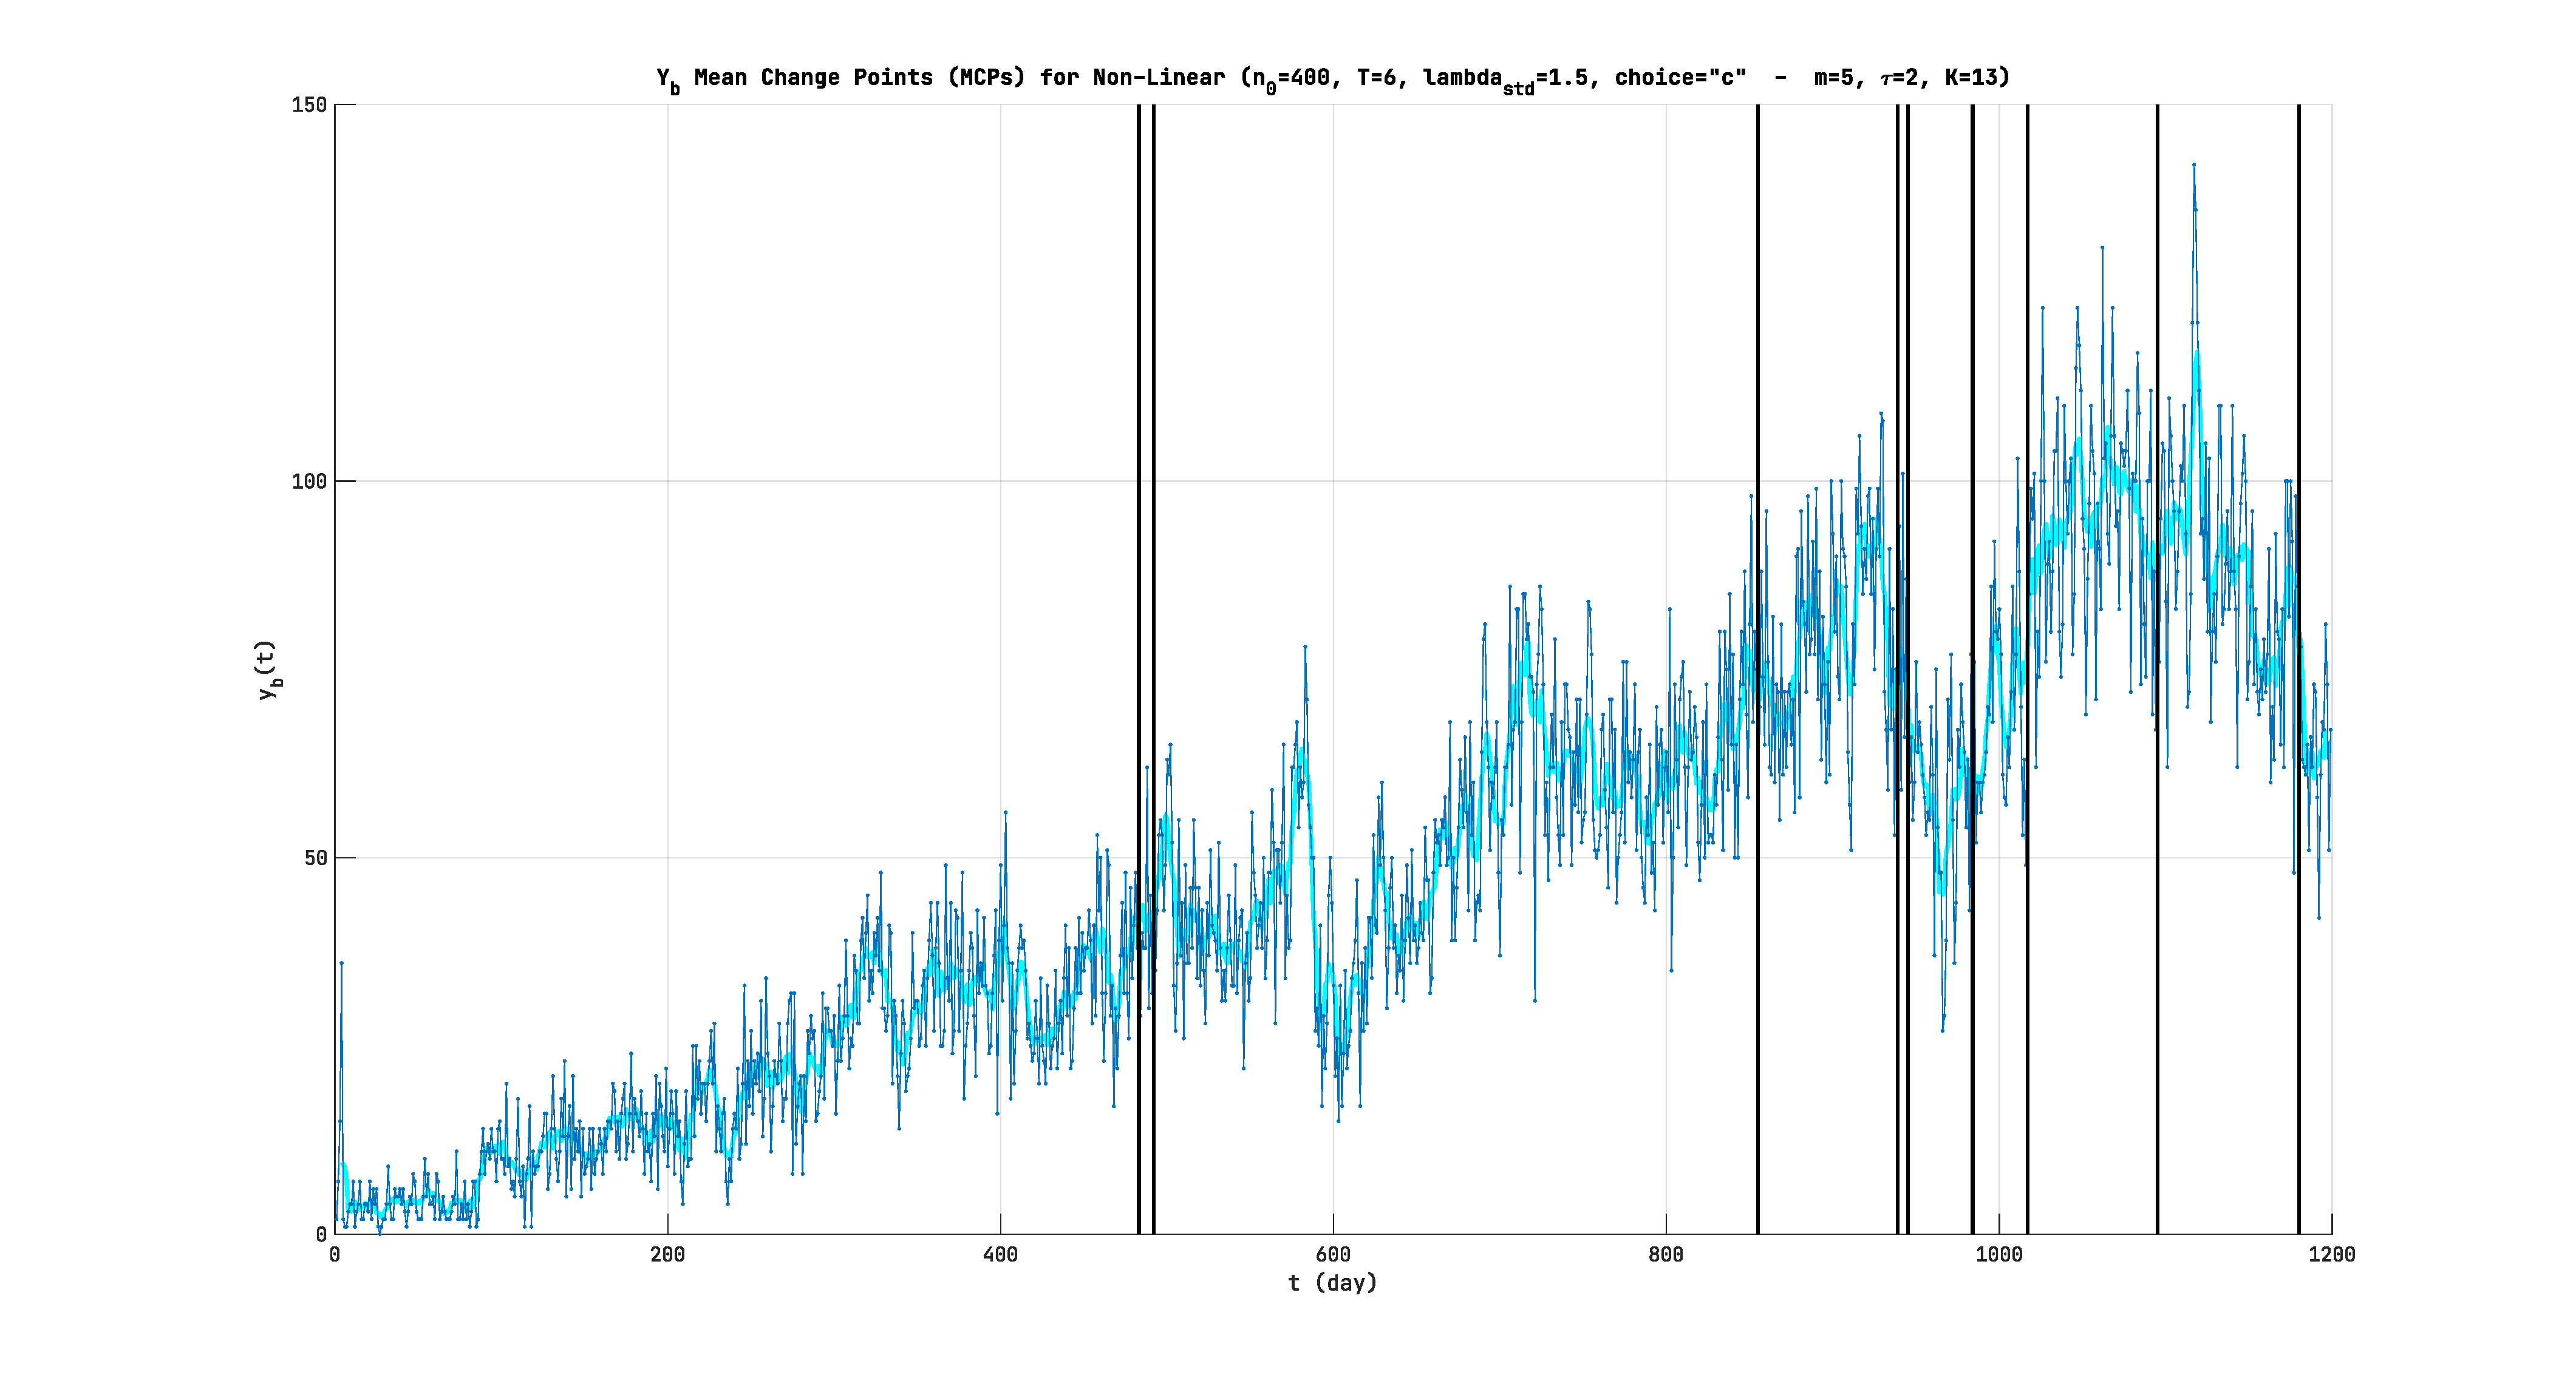
\includegraphics[width=\textwidth]{plots/mcps_nl_yb_opt_c.svg.pdf}
        \caption{Διάγραμμα ιστορίας της αρχικής χρονοσειράς $\{Y_b(t)\}$ (μπλε) μαζί με τα σημεία αλλαγής (μαύρο) που επιλέχθηκαν από τη μη-γραμμική ανάλυση της στάσιμης εκδοχής της με τις βέλτιστες παραμέτρους, καθώς και εκτίμηση της τάσης με φίλτρο κινούμενου μέσου τάξης 7 ($MA(7)$ \tl{smoothing}) - επιλογή \textquote{\tl{c}}}
        \label{fig:mcps_nl_yb_opt_c}
    \end{center}
\end{figure}

\paragraph{Αναπροσαρμογή σε κάθε χρονική στιγμή}- Επιλογή \textquote{\tl{b}}

Τα ίδια διαγράμματα παρουσιάζονται για την επιλογή αναπροσαρμογής \textquote{\tl{b}} (αναπροσαρμογή σε κάθε χρονική στιγμή) ενώ ακολουθεί σύντομος σχολιασμός:

\begin{figure}[H]
    \begin{center}
        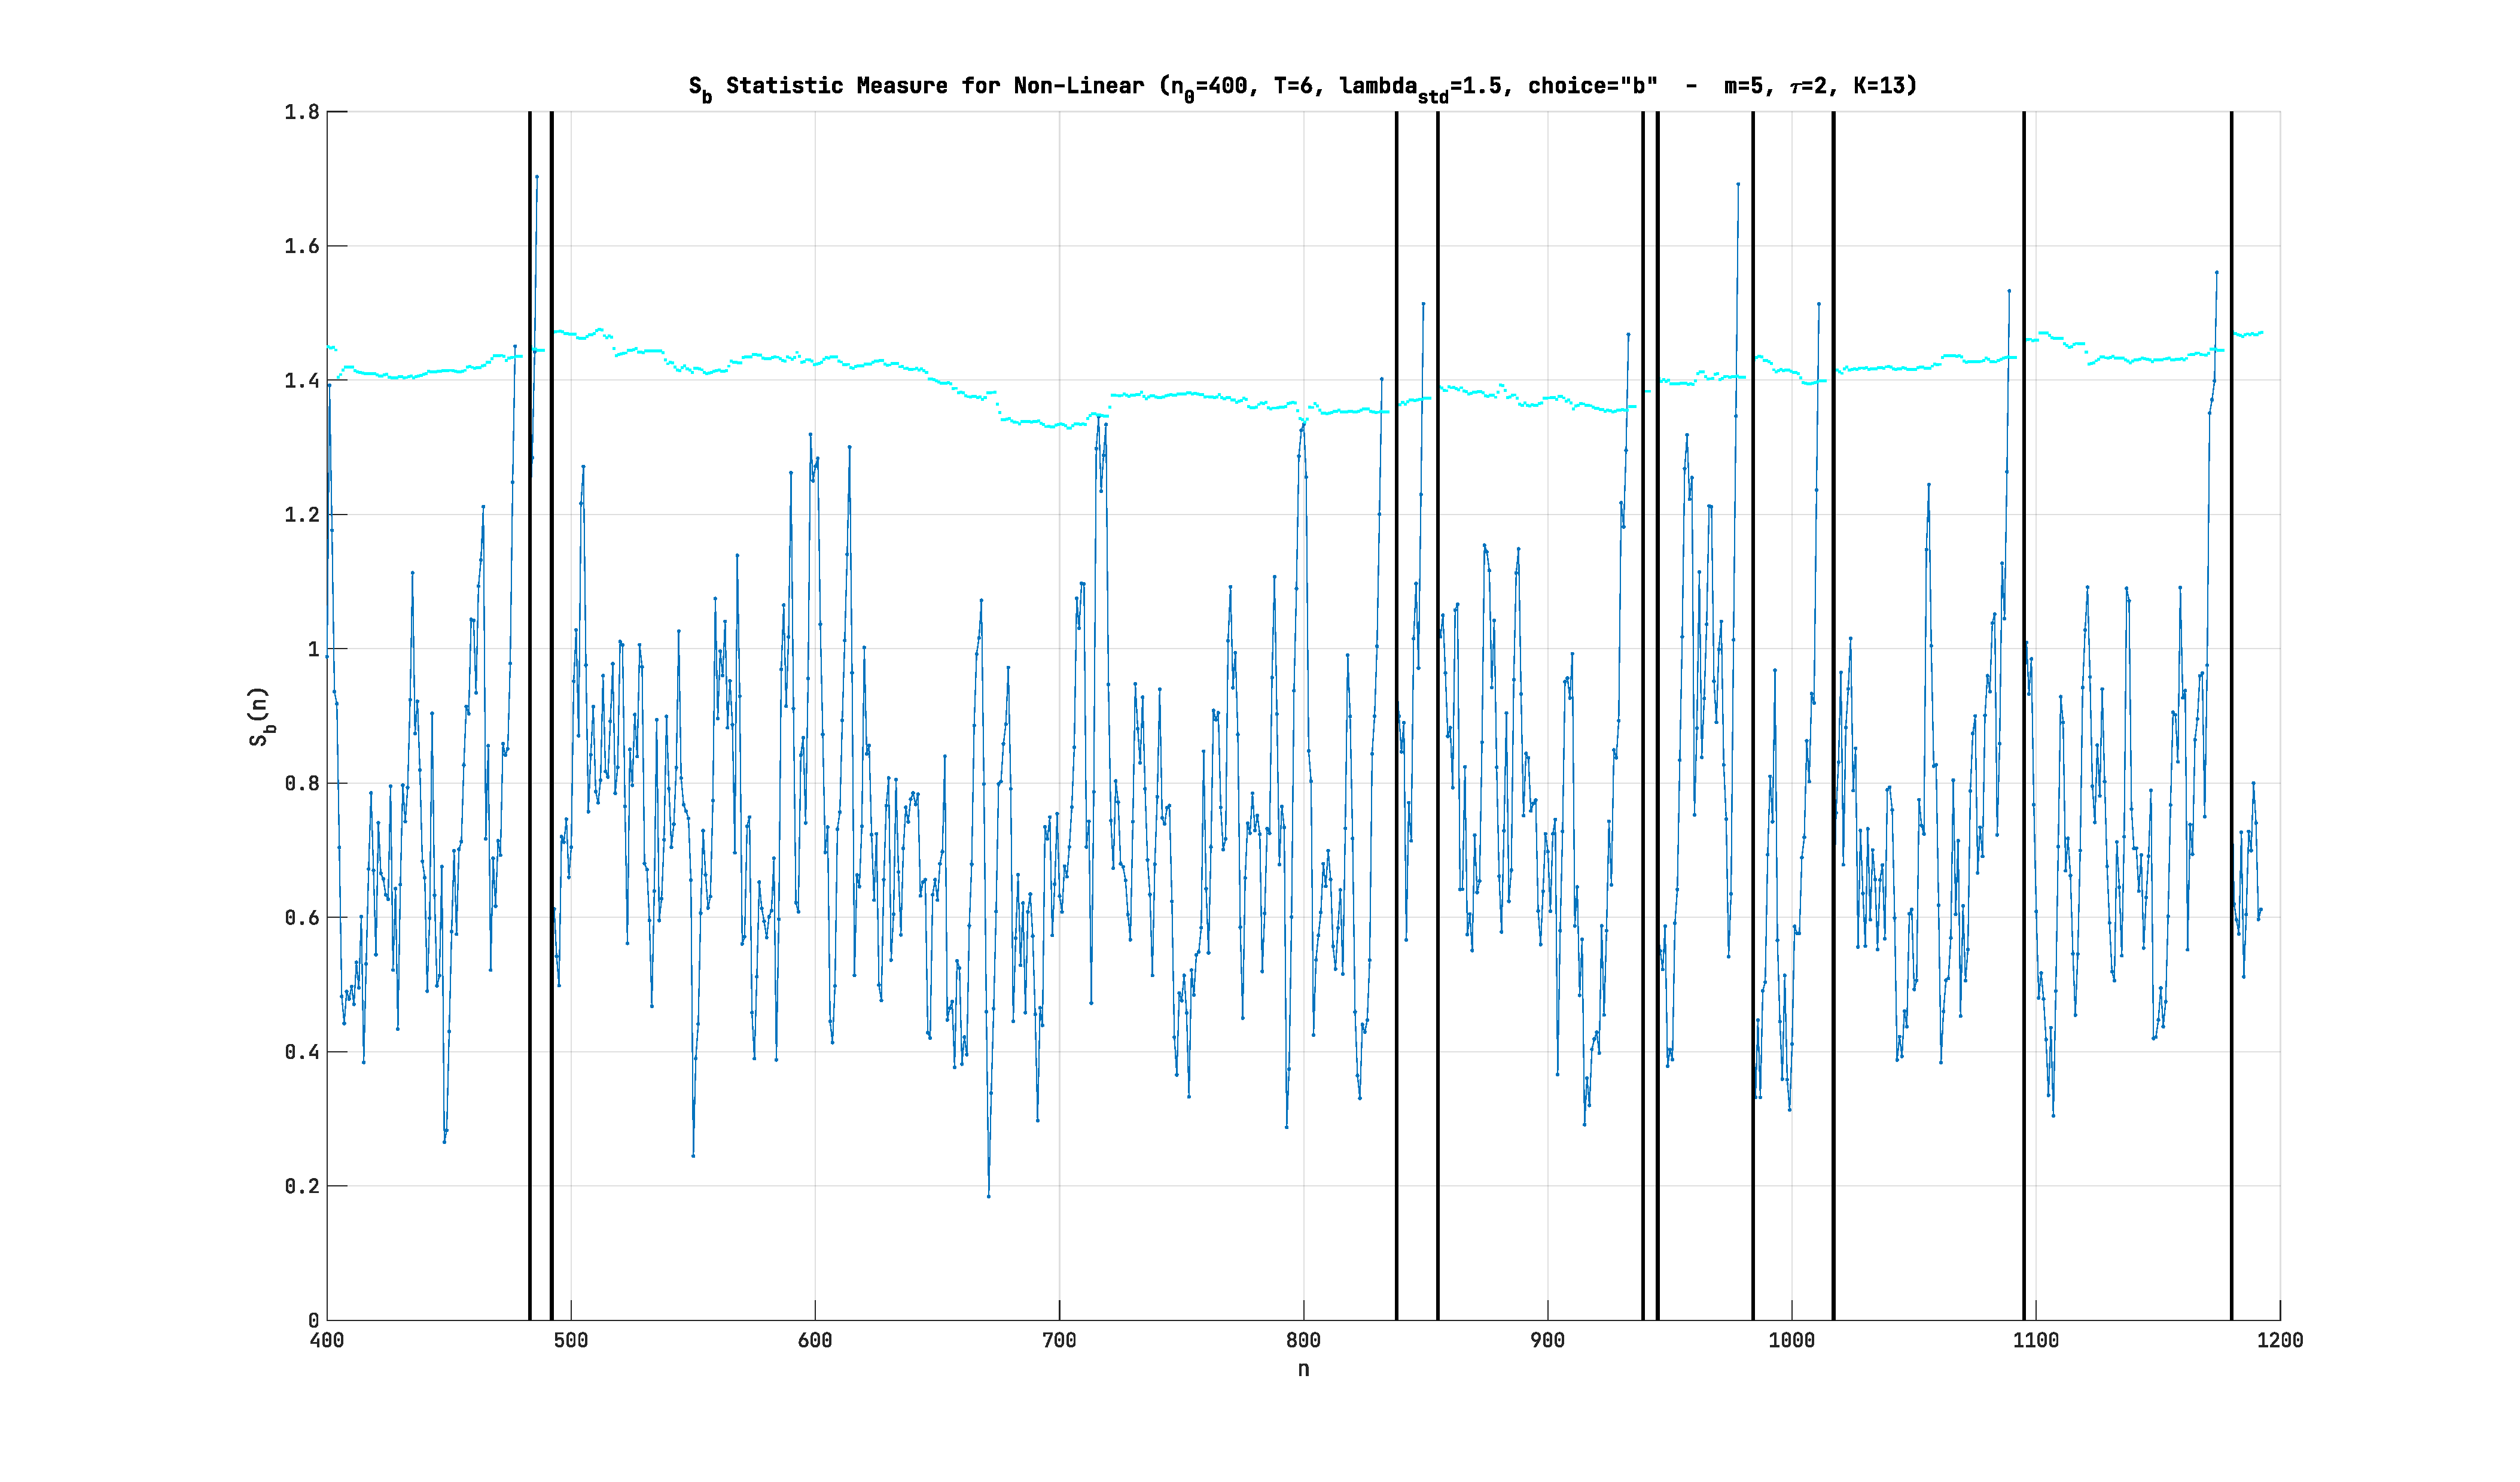
\includegraphics[width=\textwidth]{plots/mcps_nl_xb_opt_b.svg.pdf}
        \caption{Τιμές στατιστικού $S_n$ για έως και 6 βήματα μπροστά πρόβλεψη με τοπική πρόβλεψη μέσου Κ=13 κοντινότερων γειτόνων της στάσιμης χρονοσειράς $\{X_{b_{deseasoned}}(t)\}$ και για επιλογή αναπροσαρμογής \textquote{\tl{b}} (αναπροσαρμογή σε κάθε χρονική στιγμή). Σημειώνονται επίσης το κριτήριο απόφασης, $\alpha=1.5*s_x$, (\tl{cyan}) και φυσικά τα σημεία αλλαγής με έντονες κάθετες γραμμές στα εκάστοτε σημεία $n+T$ (μαύρο) - [\tl{NRMSE}=0.979, \ 0.63\tl{sec}]}
        \label{fig:mcps_nl_xb_opt_b}
    \end{center}
\end{figure}

Παρακάτω, τα ίδια σημεία αλλαγής απεικονίζονται στην αρχική χρονοσειρά προβολών του βίντεο \tl{A}:

\begin{figure}[H]
    \begin{center}
        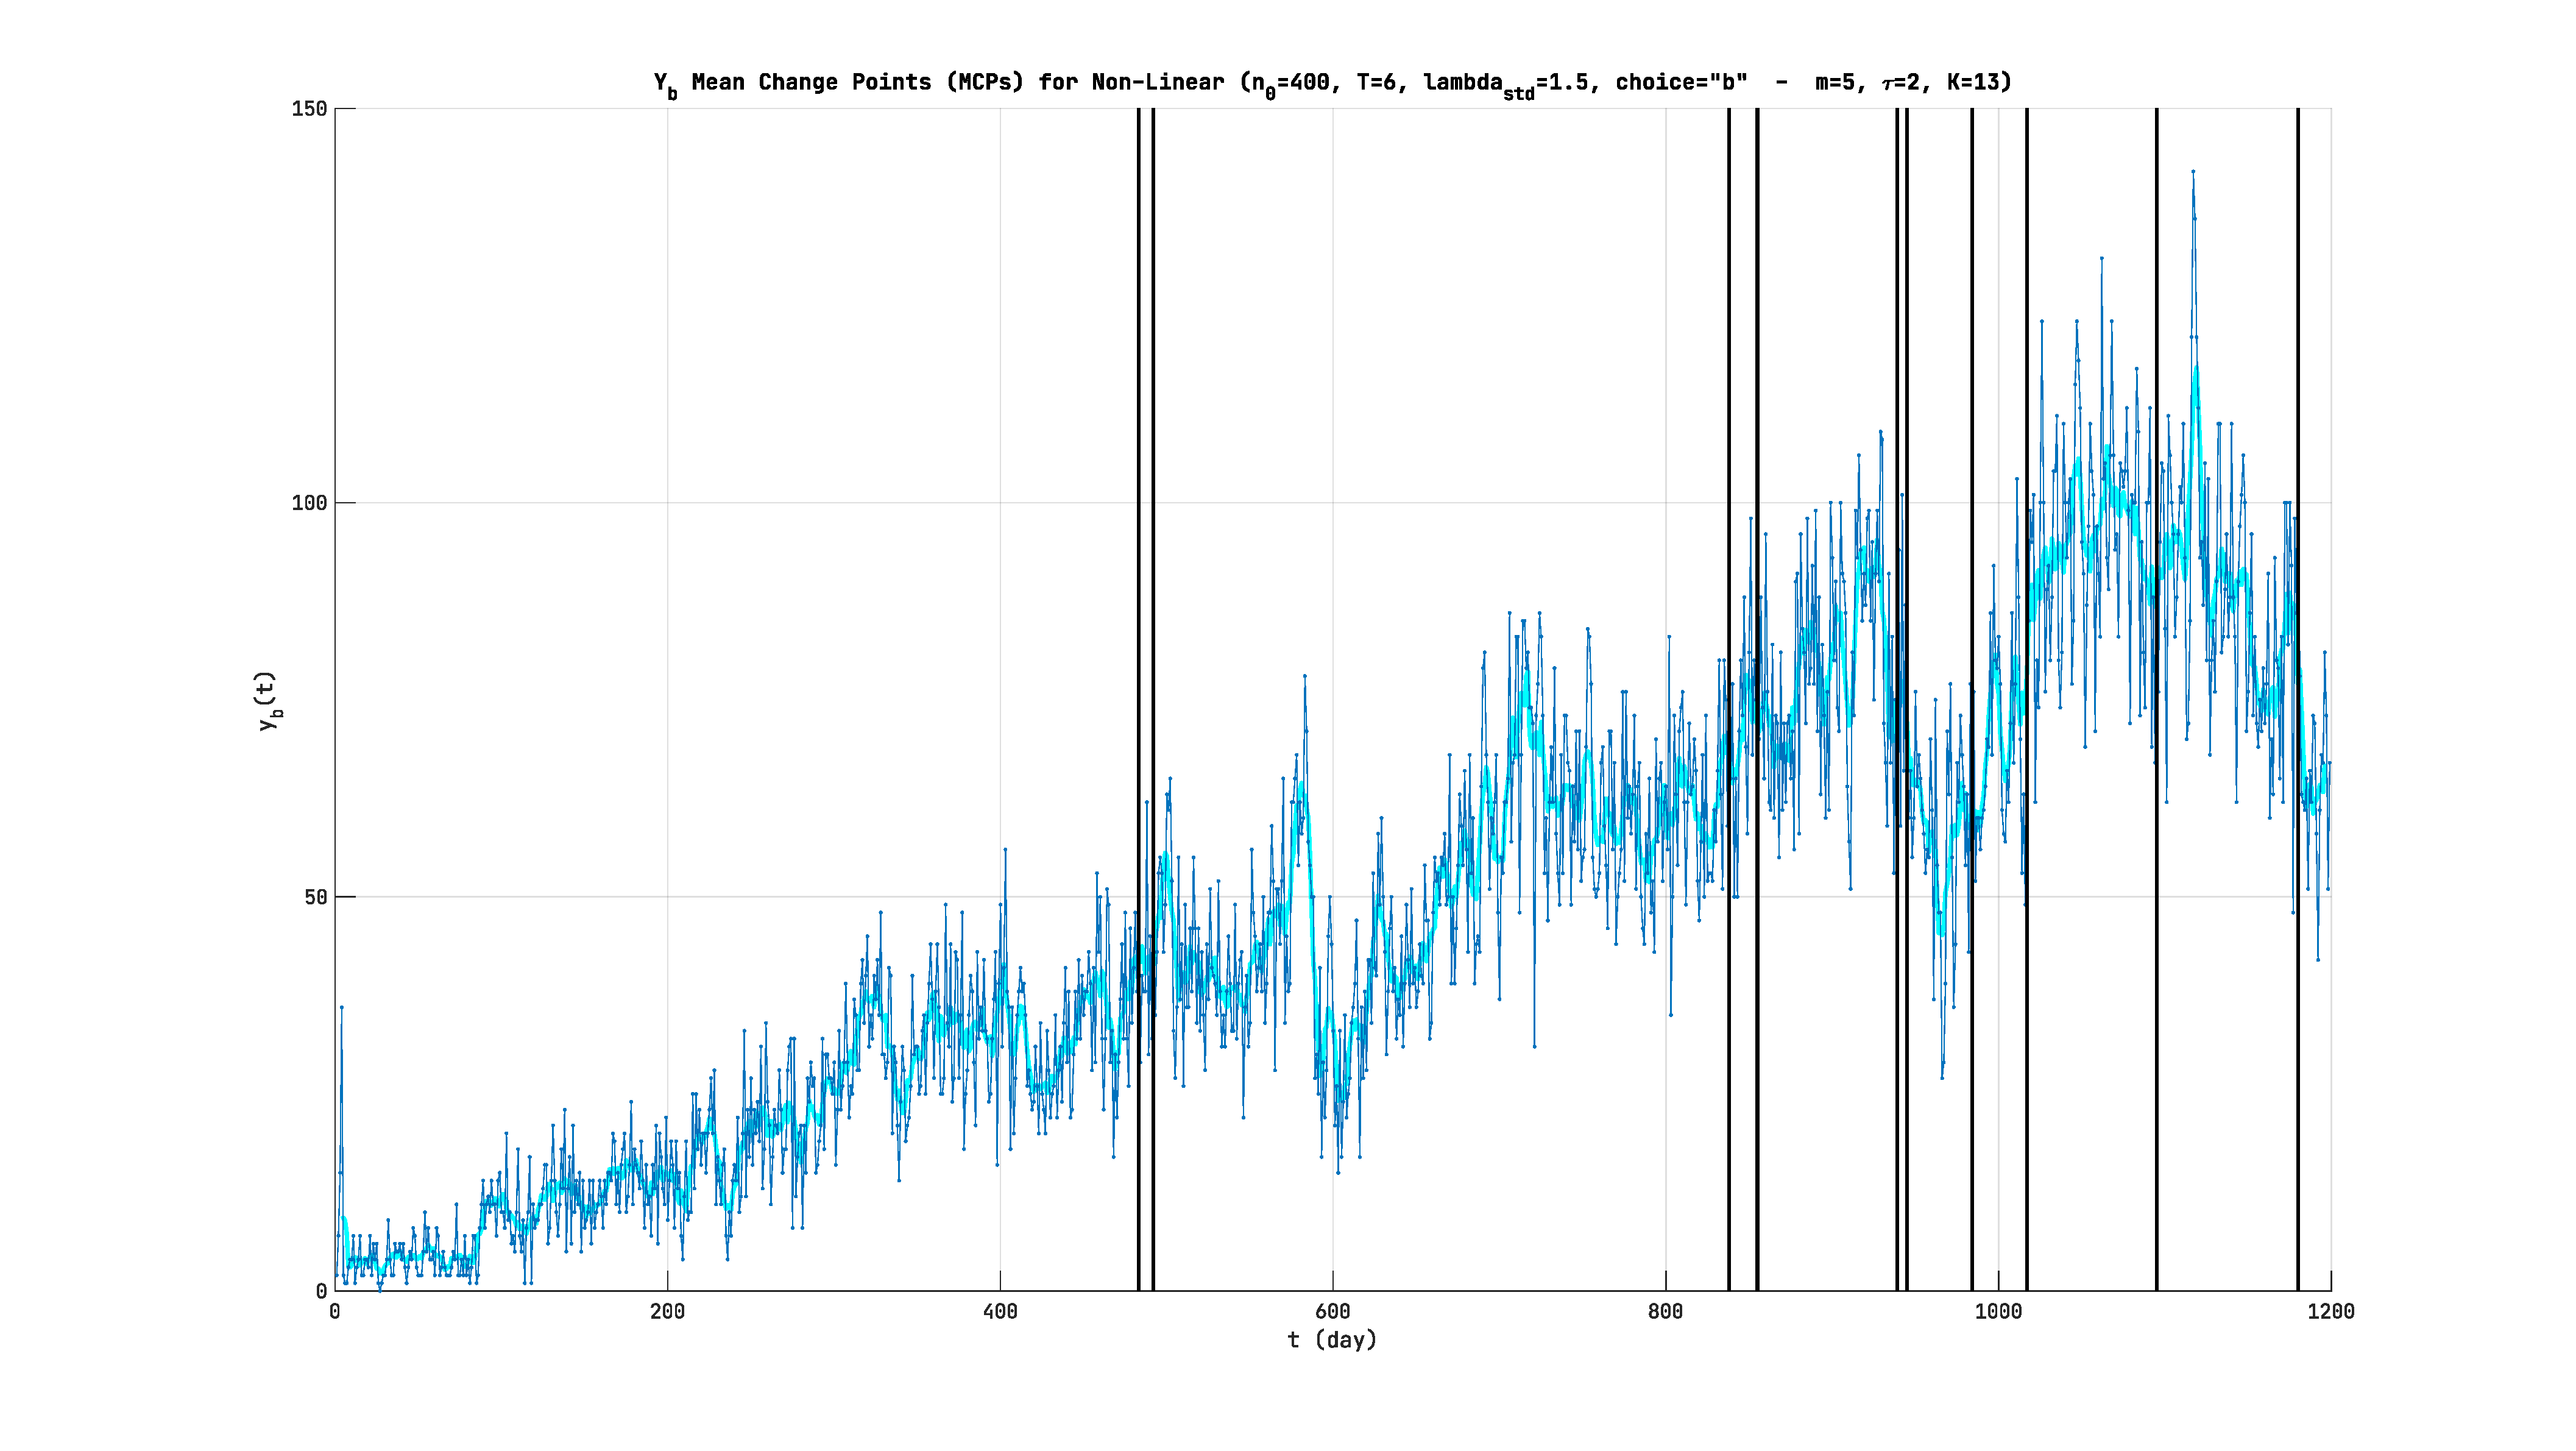
\includegraphics[width=\textwidth]{plots/mcps_nl_yb_opt_b.svg.pdf}
        \caption{Διάγραμμα ιστορίας της αρχικής χρονοσειράς $\{Y_b(t)\}$ (μπλε) μαζί με τα σημεία αλλαγής (μαύρο) που επιλέχθηκαν από τη μη-γραμμική ανάλυση της στάσιμης εκδοχής της με τις βέλτιστες παραμέτρους, καθώς και εκτίμηση της τάσης με φίλτρο κινούμενου μέσου τάξης 7 ($MA(7)$ \tl{smoothing}) - επιλογή \textquote{\tl{b}}}
        \label{fig:mcps_nl_yb_opt_b}
    \end{center}
\end{figure}

Φαίνεται η κυμάτωση του ορίου απόφαση καθώς αυτό επαναϋπολογίζεται σε κάθε χρονική στιγμή. Επίσης, βλέπουμε πως έχει βγει ακόμα ένα σημείο αλλαγής λόγω αυτής της μεταβολής και πλέον είναι 10. Επίσης υπάρχει μικρή αύξηση του \tl{NRMSE}.

\paragraph{Χωρίς Αναπροσαρμογή}- Επιλογή \textquote{\tl{a}}

Τέλος, τα ίδια διαγράμματα παρουσιάζονται για την επιλογή αναπροσαρμογής \textquote{\tl{a}} (καμία αναπροσαρμογή - διατήρηση της τυπικής απόκλισης / ορίου απόφασης που υπολογιστήκε από τις πρώτες 400 παρατηρήσεις της στάσιμης χρονοσειράς), ενώ ακολουθεί σύντομος σχολιασμός:

\begin{figure}[H]
    \begin{center}
        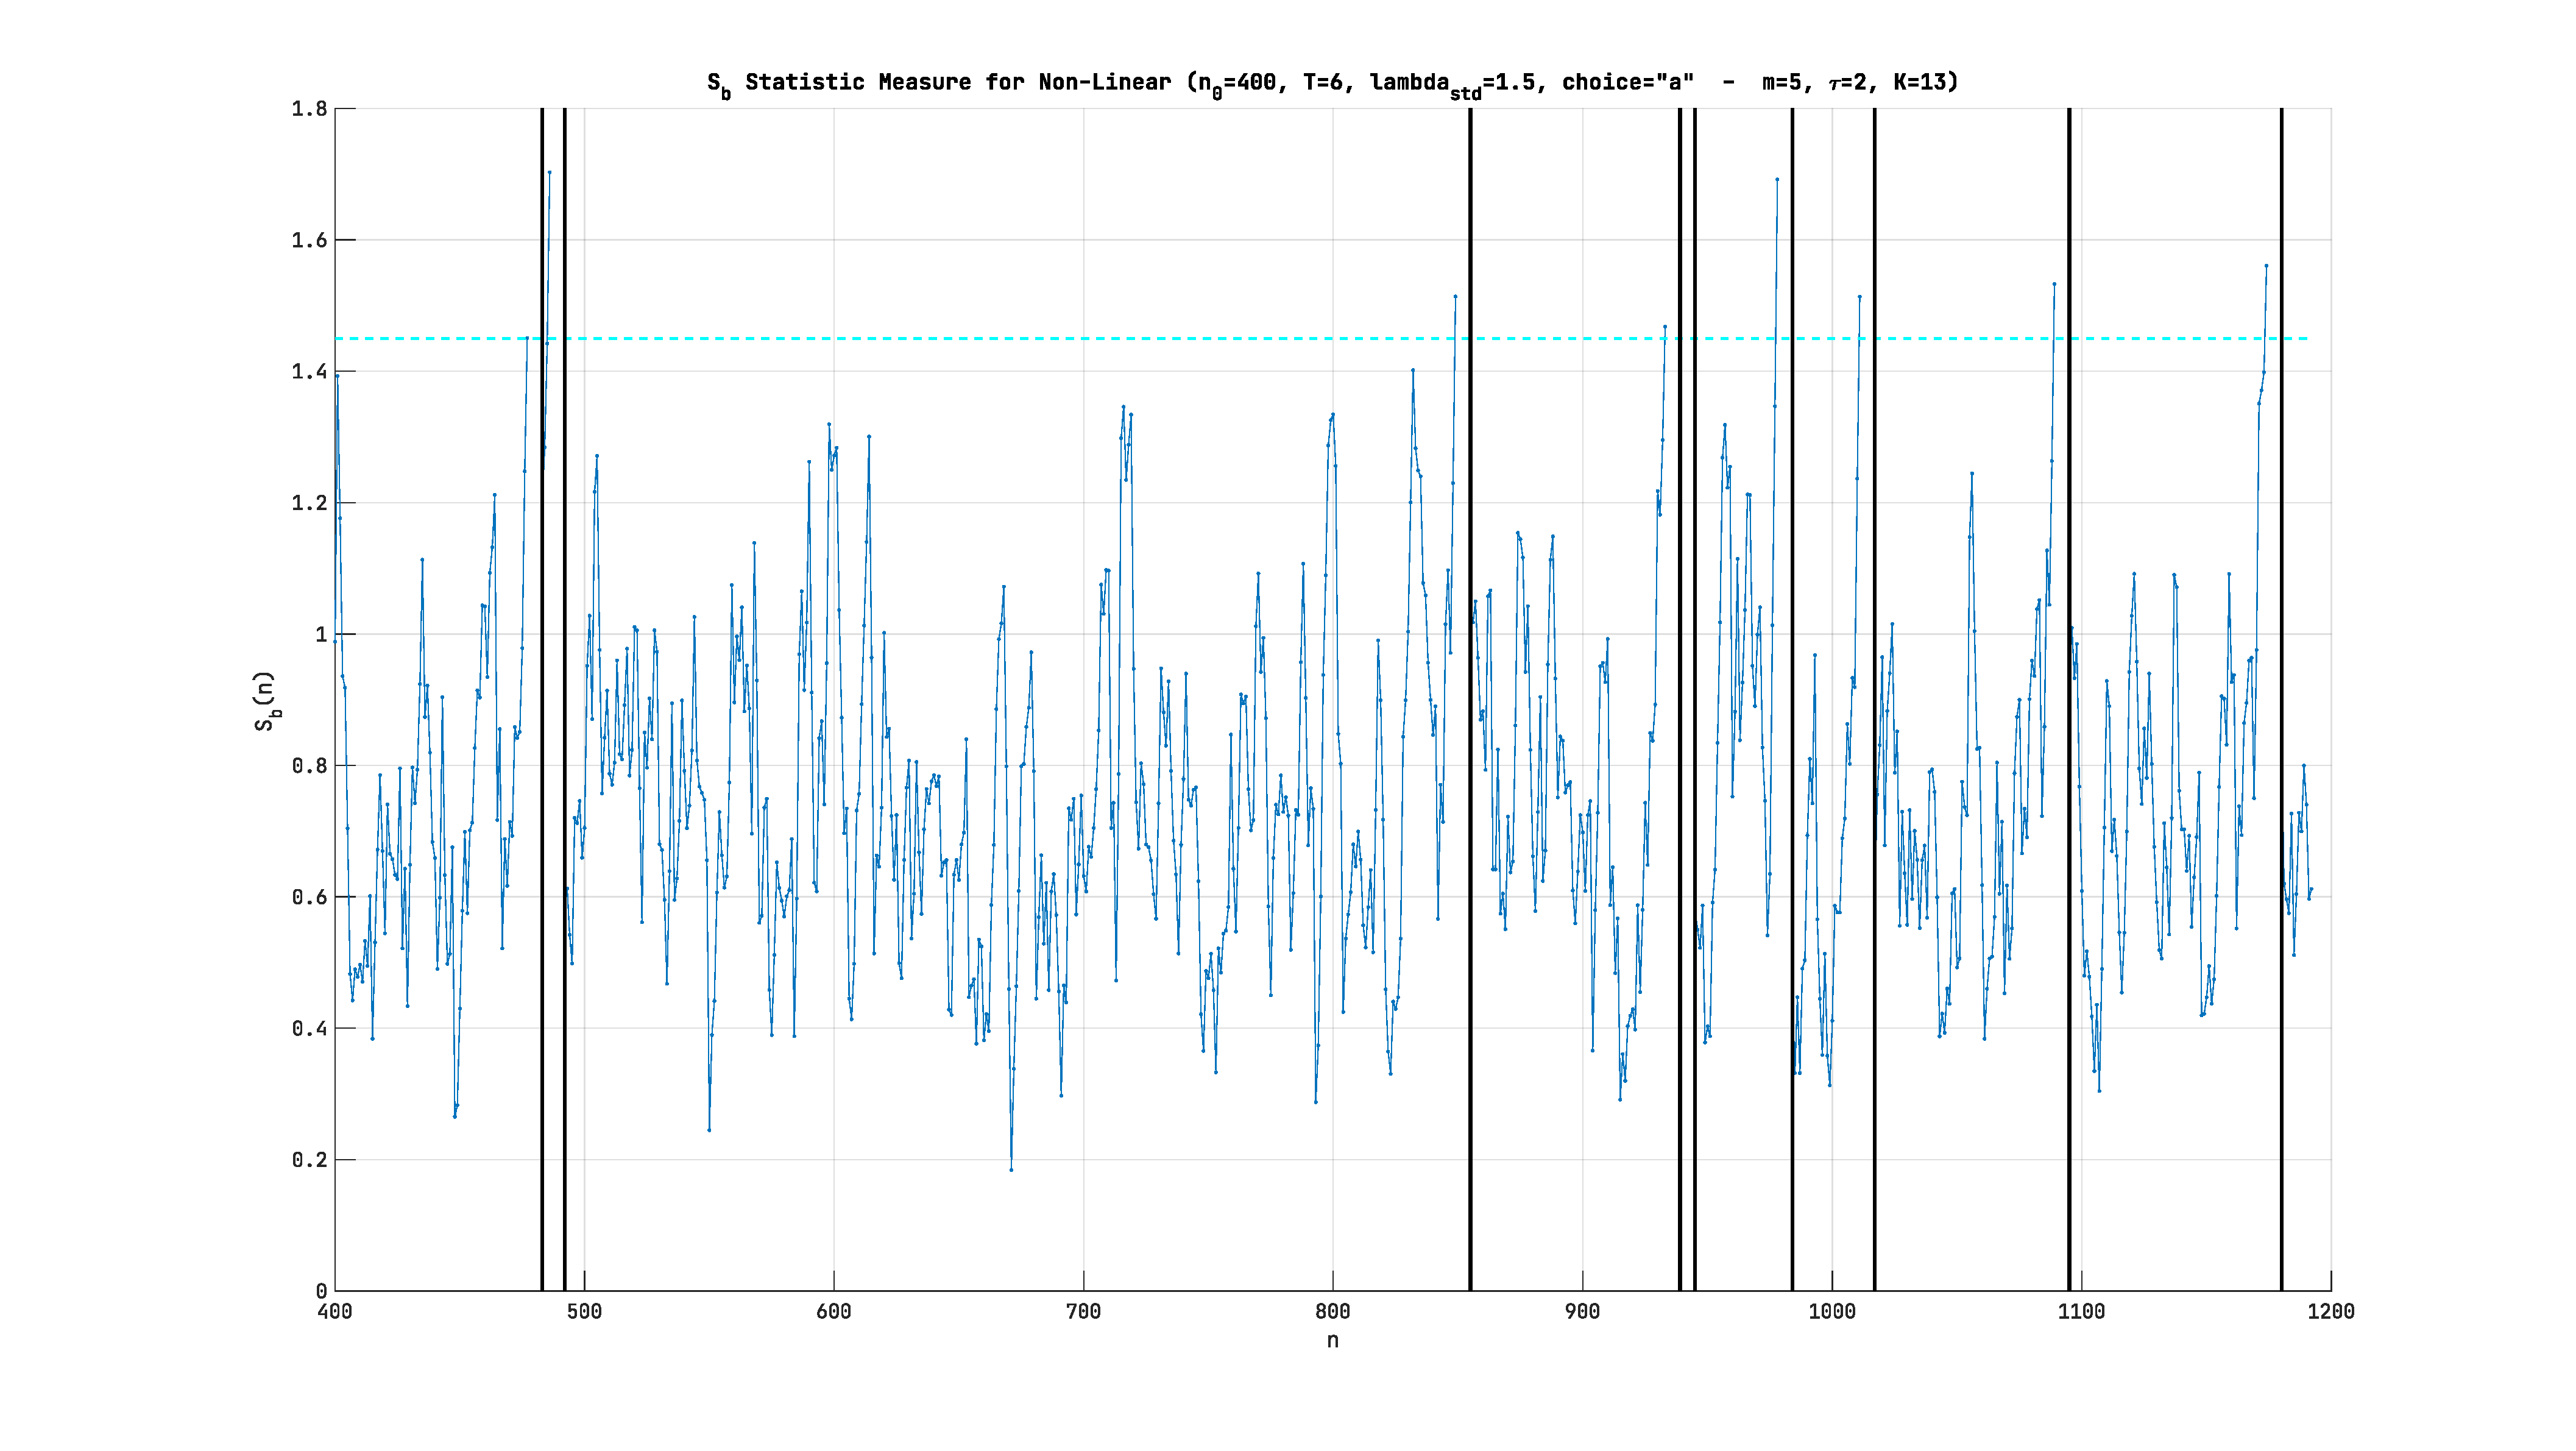
\includegraphics[width=\textwidth]{plots/mcps_nl_xb_opt_a.svg.pdf}
        \caption{Τιμές στατιστικού $S_n$ για έως και 6 βήματα μπροστά πρόβλεψη με τοπική πρόβλεψη μέσου Κ=13 κοντινότερων γειτόνων της στάσιμης χρονοσειράς $\{X_{b_{deseasoned}}(t)\}$ και για επιλογή αναπροσαρμογής \textquote{\tl{a}} (χωρίες αναπροσαρμογή). Σημειώνονται επίσης το κριτήριο απόφασης, $\alpha=1.5*s_x$, (\tl{cyan}) και φυσικά τα σημεία αλλαγής με έντονες κάθετες γραμμές στα εκάστοτε σημεία $n+T$ (μαύρο) - [\tl{NRMSE}=0.975, \ 0.61\tl{sec}]}
        \label{fig:mcps_nl_xb_opt_a}
    \end{center}
\end{figure}

Παρακάτω, τα ίδια σημεία αλλαγής απεικονίζονται στην αρχική χρονοσειρά προβολών του βίντεο \tl{A}:

\begin{figure}[H]
    \begin{center}
        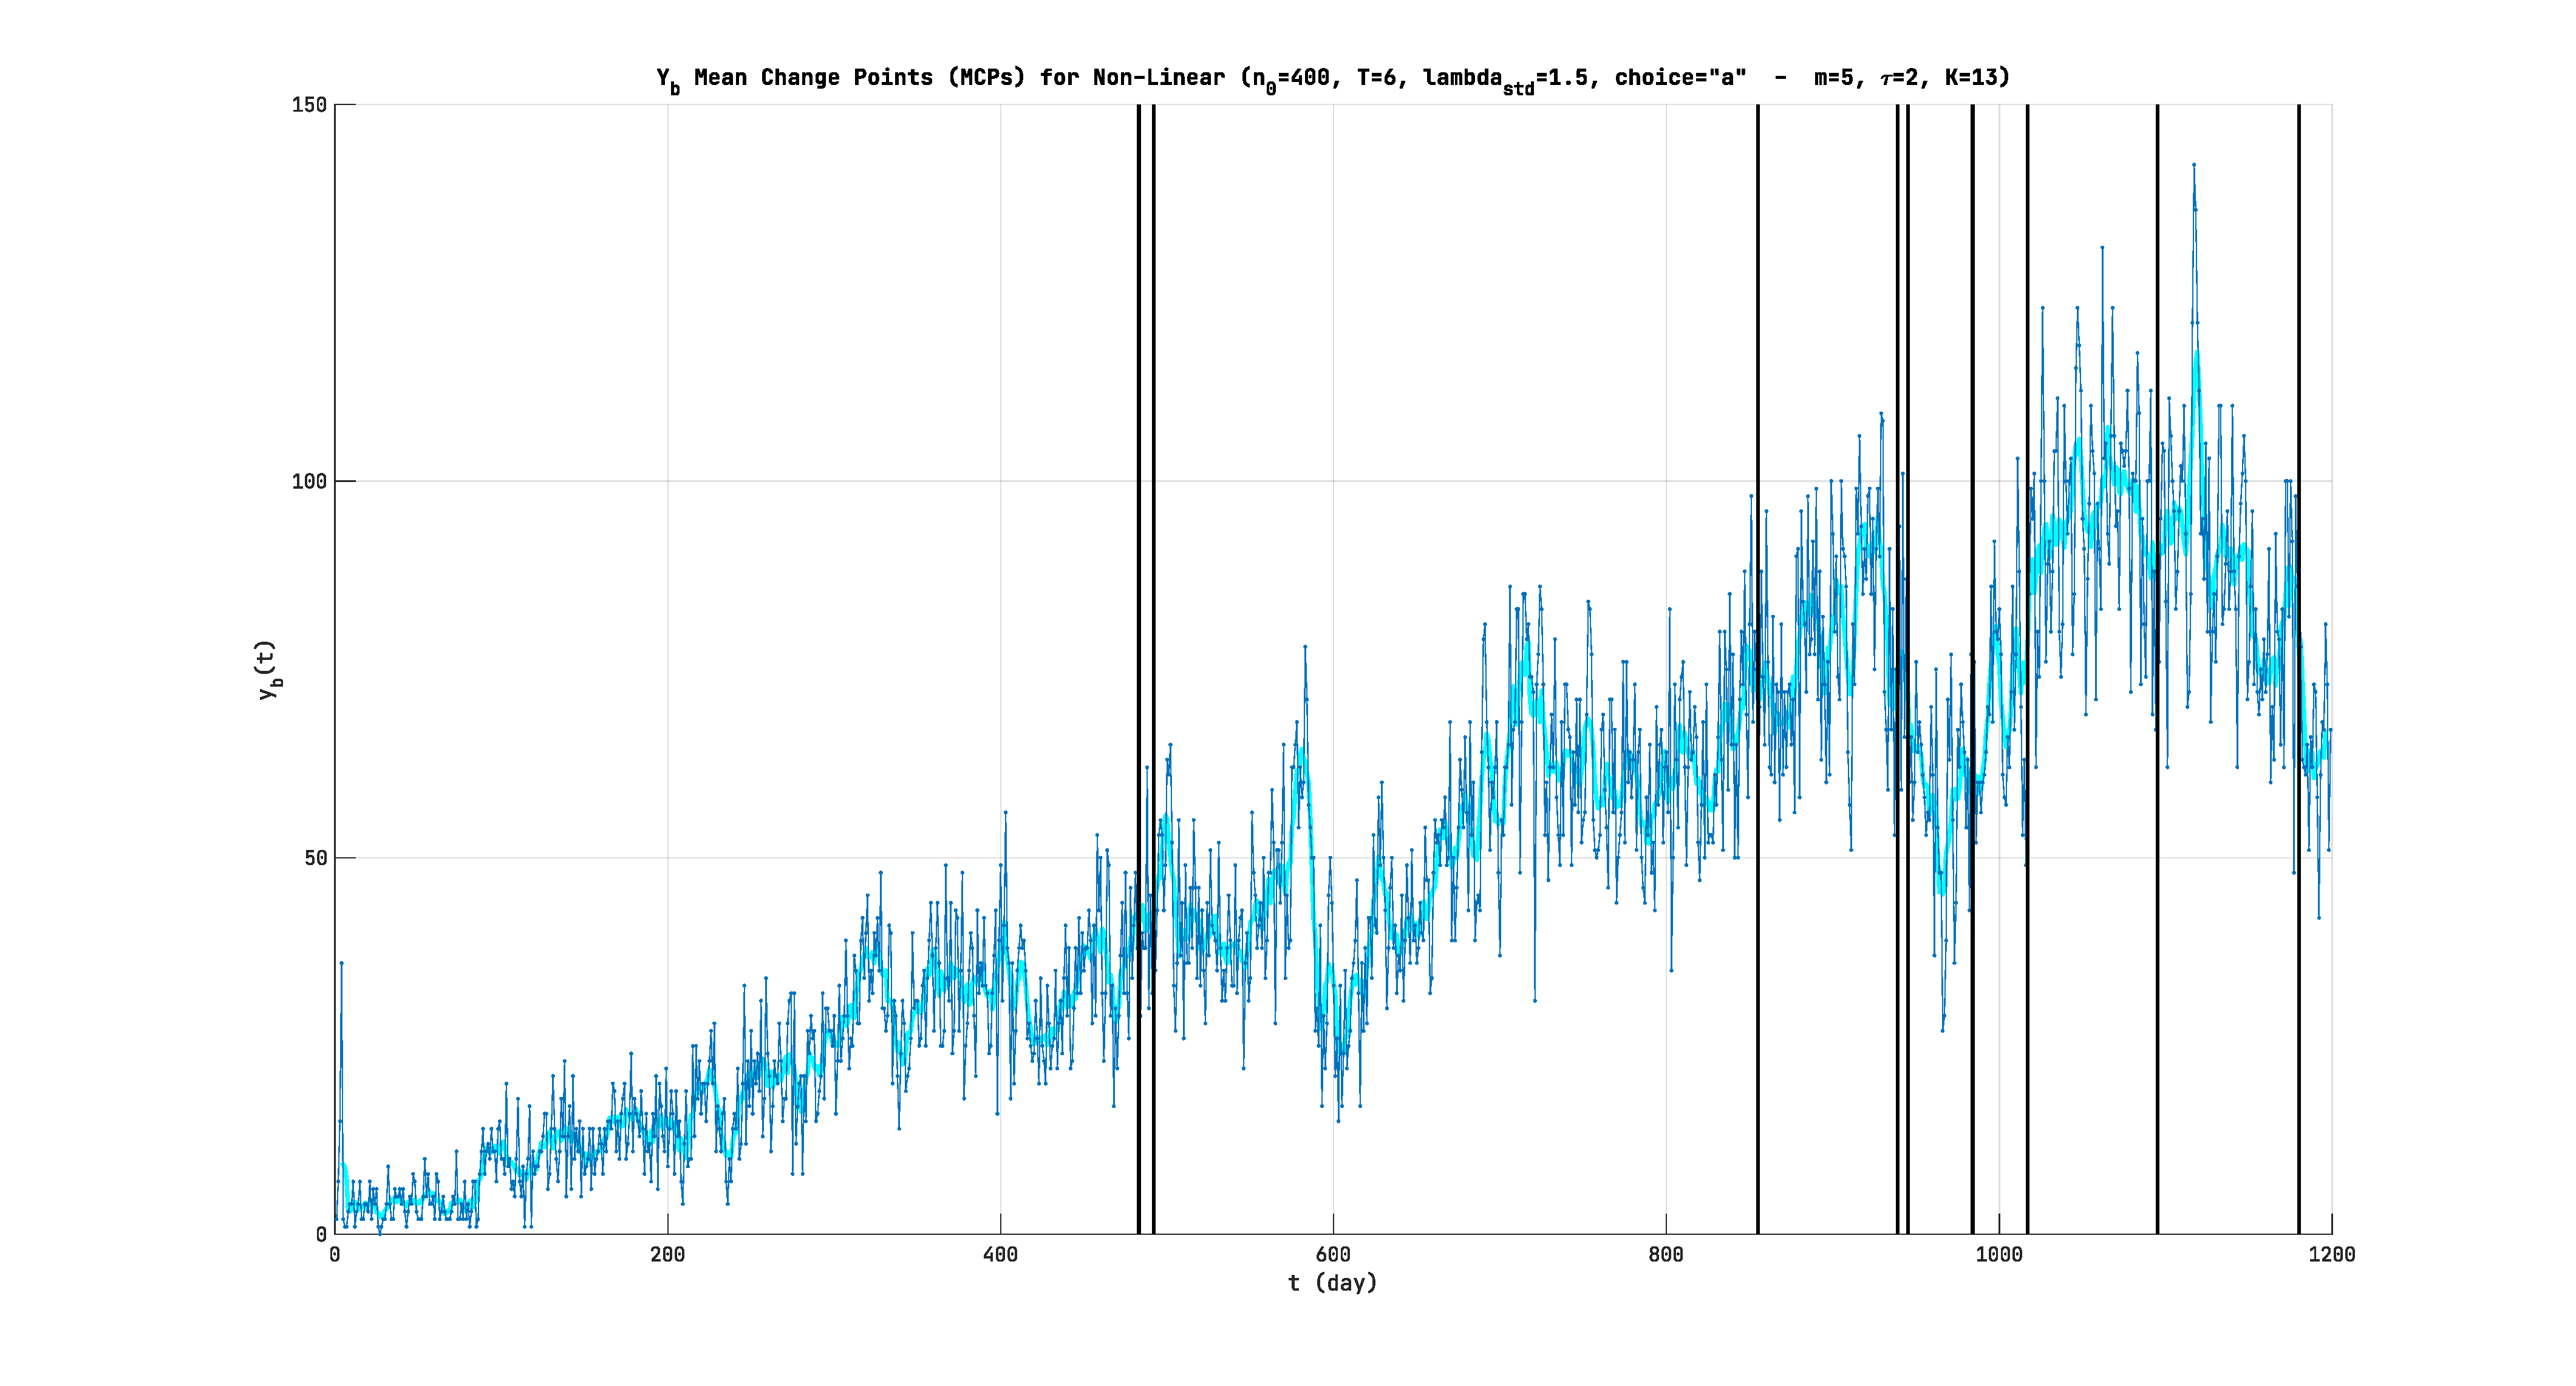
\includegraphics[width=\textwidth]{plots/mcps_nl_yb_opt_a.svg.pdf}
        \caption{Διάγραμμα ιστορίας της αρχικής χρονοσειράς $\{Y_b(t)\}$ (μπλε) μαζί με τα σημεία αλλαγής (μαύρο) που επιλέχθηκαν από τη μη-γραμμική ανάλυση της στάσιμης εκδοχής της με τις βέλτιστες παραμέτρους, καθώς και εκτίμηση της τάσης με φίλτρο κινούμενου μέσου τάξης 7 ($MA(7)$ \tl{smoothing}) - επιλογή \textquote{\tl{a}}}
        \label{fig:mcps_nl_yb_opt_a}
    \end{center}
\end{figure}

Τα σημεία αλλαγής είναι τα ίδια σε αριθμό και σε θέσεις με αυτά της επιλογής \textquote{\tl{c}}. Ίδιος είναι επίσης ο χρονος εκτέλεσης και το \tl{NRMSE}.

\par \textit{Γενικότερα, και για τη χρονοσειρά Β, όσο μειώνονται τα σημεία αλλαγής που βγάζει η μέθοδος (μέχρι καποιο σημείο) τόσο και το \tl{NRMSE} των προβλέψεων κατά την εφαρμογή της μεθόδου μειώνεται.\\
Συγκρίνοντας τα σημεία αλλαγής με τα αντίστοιχα από τη γραμμική πρόβλεψη και ανάλυση του βήματος \ref{ch:step4} βλέπουμε ότι \textbf{δεν υπάρχει έντονη συνέπεια} στις θέσεις όπου εντοπίζονται σημεία αλλαγής, δηλαδή στο μη-γραμμικό μοντέλο πρόβλεψης δεν είνα πάντα γύρω από τοπικες \textquote{εξάρσεις} ή τοπικές \textquote{βυθίσεις} της αρχικής χρονοσειράς προβολών του βίντεο Β. Επίσης, επειδή \textbf{η επιλογή σημείων αλλαγής με γραμμικό μοντέλο πρόβλεψης} αφήνει μικρότερο \tl{NRMSE}, θα λέγαμε πως και για τη δεύτερη χρονοσειρά \textbf{υπερτερεί} έναντι της χρήσης μη-γραμμικού τοπικού μοντέλου κοντινότερων γειτόνων.}